\documentclass[9pt]{report}

\usepackage[a4paper,left=1.3cm,right=1.5cm,top=3cm,bottom=2.5cm,bindingoffset=5mm]{geometry}
\usepackage[ngerman,english]{babel}
\usepackage[utf8]{inputenc}
\usepackage[T1]{fontenc}
\usepackage{lmodern}
\usepackage{amsmath}
\usepackage{amssymb}
\usepackage{bbm}
\usepackage{tabularx}
\usepackage{graphicx}
\usepackage{siunitx}
\usepackage{array}
\usepackage{ragged2e}
\usepackage{hyperref}
\usepackage{float}
\usepackage{floatflt}
\usepackage{listings}
\usepackage{color}
\usepackage[font=small]{caption, subcaption}
\usepackage[dvipsnames]{xcolor}
\usepackage[theorems]{tcolorbox}
\usepackage{fancyhdr}
\usepackage{autobreak}
\usepackage{wrapfig}
\usepackage{lipsum}
\usepackage{calc}
%\usepackage{picins}


\pagestyle{fancy}

\fancyhf{}

\lhead{\rightmark}
\chead{}
\rhead{\thepage}

\lfoot{}
\cfoot{}
\rfoot{}



\newcommand{\op}{
	\mathop{
		\vphantom{\bigoplus} 
		\mathchoice
		{\vcenter{\hbox{\resizebox{\widthof{$\displaystyle\bigoplus$}}{!}{$\boxplus$}}}}
		{\vcenter{\hbox{\resizebox{\widthof{$\bigoplus$}}{!}{$\boxplus$}}}}
		{\vcenter{\hbox{\resizebox{\widthof{$\scriptstyle\oplus$}}{!}{$\boxplus$}}}}
		{\vcenter{\hbox{\resizebox{\widthof{$\scriptscriptstyle\oplus$}}{!}{$\boxplus$}}}}
	}\displaylimits 
}




\lstset{language=Python, 
        columns=flexible, 
        numbers=left, 
        xleftmargin=1.3em, 
        basicstyle=\footnotesize\ttfamily, 
        keywordstyle=\color{blue}, 
        morekeywords={as}, 
        stringstyle=\color{green}}


%\tcbset{defstyle/.style={
%		fonttitle=\sffamily\bfseries,
%		arc=0mm,
%		colback=blue!10,
%		colframe=green,
%		separator sign none}}




\title{\Huge\textbf{Quantum Dynamics}}
\date{}
\author{}










\begin{document}

\maketitle


\tableofcontents















\newpage
\chapter{Quantum Statistical Mechanics}


\section{Thermal De Broglie wavelength}
\url{https://www.youtube.com/watch?v=EtKtYRmMF8Y}


\section{Statistical Definition of Observables}
In der statistischen Mechanik ist ein \textbf{Mikrozustand} durch eine vollständige mikroskopische Beschreibung des Systems definiert. Meist geht man von der zeitunabhängigen Schrödingergleichung
\begin{equation}
\hat{H}|\Psi_{\nu}\rangle = E_{\nu}|\Psi_{\nu}\rangle
\end{equation}
aus und wählt als Mikrozustände die Eigenzustände des Hamiltonoperators. Für ein System mit $f$ Freiheitsgraden hängen sie von $f$ Quantenzahlen $n_k$ ab:
\begin{equation}
\mathrm{Mikrozustand}:\;\nu=(n_1,n_2,...,n_f)
\end{equation}
Im Allgemeinen gibt es in einem System unendlich viele Mikrozustände $\nu$, da mindestens eine Quantenzahl unendlich viele Werte annehmen kann. Bei vorgegebener Energie ist die Anzahl der möglichen Mikrozustände aber endlich.

Es ist in der Regel unmöglich, den tatsächlichen Mikrozustand eines makroskopischen Vielteilchensystems anzugeben. Relevant ist aber, welche Mikrozustände mit welchem statistischen Gewicht auftreten. Der Zustand eines Systems kann also durch die Angabe der Wahrscheinlichkeiten $P_{\nu}$ für die Mikrozustände $\nu$ vollständig beschrieben werden. Der so festgelegte Zustand des Systems heißt \textbf{Makrozustand}:
\begin{equation}
\mathrm{Makrozustand}:\;\{P_{\nu}\}=(P_1,P_2,P_3,...)
\end{equation}
Die Definition einer Wahrscheinlichkeit $P_{\nu}$ eines Mikrozustands setzt eine große Anzahl $A$ gleichartiger Systeme voraus, von denen $a_{\nu}$ im Mikrozustand $\nu$ sind:
\begin{equation}
P_{\nu}=\lim_{A\to\infty}\frac{a_{\nu}}{A}\approx \frac{a_{\nu}}{A}
\end{equation}
Die Gesamtheit der $\mathcal{N}$ gleichartigen Systeme, die die $P_{\nu}$ festlegen, nennt man \textbf{statistisches Ensemble}. Insgesamt gibt es
\begin{equation}
\Gamma(P_1,P_2,...) = \frac{A!}{a_1!\,a_2!\cdots a_{k}!}=\frac{A!}{\displaystyle\prod_{\nu}a_{\nu}!}
\end{equation}
Möglichkeiten, $A$ Systeme auf $\nu$ Boxen so zu verteilen, sodass sich in der $\nu$-ten Box gerade $a_{\nu}$ Systeme befinden, die im Mikrozustand $\nu$ sind. Damit ist $\Gamma$ die Anzahl möglicher Ensemblezustände, die proportional zur Anzahl möglicher Mikrozustände ist. Die \textbf{Entropie} ist ein Maß für die Menge an Information, die benötigt wird, um von einem gegebenen Makrozustand auf den gerade vorliegenden Ensemblezustand schließen zu können. Betrachtet man Makrozustände $\{P_1,P_2,...P_{\nu}\}$ mit unterschiedlich vielen möglichen Mikrozuständen $\nu$, dann erkennt man, dass die oben beschriebene Informationsmenge logarithmisch mit der Anzahl von Mikro- und damit Ensemblezuständen wächst. Daher kann man mit Hilfe der Stirling-Approximation
\begin{equation}
\ln A! \approx A\ln A -A\qquad\mathrm{und} \qquad\sum_{\nu}a_{\nu} =A
\end{equation}
den natürlichen Logarithmus von $\Gamma(P_1,P_2,...)$ bilden und gelangt so zur Definition der Entropie für ein Ensemble aus $\mathcal{N}$ Systemen:
\begin{align}
\ln\Gamma(P_1,P_2,...) &= \ln\frac{A!}{\displaystyle\prod_{\nu}a_{\nu}!} =\ln A! -\sum_{\nu}\ln A!\\
&= A\ln A-A-\sum_{\nu}a_{\nu}\ln a_{\nu}+\sum_{\nu}a_{\nu}\\
&= \sum_{\nu}a_{\nu}\ln A - \sum_{\nu}a_{\nu}\ln a_{\nu} = -\sum_{\nu}a_{\nu}(\ln a_{\nu}-\ln A)\\
&= -\sum_{\nu}a_{\nu}\ln\frac{a_{\nu}}{A} = -A\sum_{\nu}P_{\nu}\ln P_{\nu} = S_{A}
\end{align}
Um die Entropie $S$ \textit{eines} Systems zu erhalten, teilt man durch den Proportionalitätsfaktor $\mathcal{N}$ und erhält:
\begin{equation}
S(P_1,P_2,...) =-k_{\mathrm{B}}\sum_{\nu}P_{\nu}\ln P_{\nu}=-k_{\mathrm{B}}\big\langle\ln P\big\rangle\label{Entropy formula}
\end{equation}
Dabei ist $\ln P_{\nu}$ als der Informationsgehalt des $\nu$-ten Mikrozustands definiert, gewichtet mit der Wahrscheinlichkeit $P_{\nu}$, mit der dieser Mikrozustand auftritt. Dieser Mittelwert wird auch \textbf{Gibbs-Entropie} genannt. Im Allgemeinen können viele Observablen $O$ in der Statistischen Mechanik als Mittelwerte über die Mikrozustände $|\Psi_{\nu}\rangle$ definiert werden:
\begin{equation}
\langle O\rangle = \sum_{\nu}P_{\nu}O_{\nu}
\end{equation}
In der Quantenstatistik wird der Wert der Observablen $O_{\nu}$ im Mikrozustand $|\Psi_{\nu}\rangle$ ersetzt durch den Erwartungswert des zugehörigen Operators $\langle\hat{O}\rangle=\langle\Psi_{\nu}|\hat{O}|\Psi_{\nu}\rangle$. Damit erhält man:
\begin{align}
\langle\langle\hat{O}\rangle\rangle &= \sum_{\nu}P_{\nu}\langle\Psi_{\nu}|\hat{O}|\Psi_{\nu}\rangle = \sum_{\nu}P_{\nu}\langle\Psi_{\nu}|\hat{O}\hat{\mathbbm{1}}|\Psi_{\nu}\rangle\\
&= \sum_{\nu}P_{\nu}\langle\Psi_{\nu}|\hat{O}\sum_{i}|i\rangle\langle i|\Psi_{\nu}\rangle= \sum_{\nu}\sum_{i}P_{\nu}\langle\Psi_{\nu}|\hat{O}|i\rangle\langle i|\Psi_{\nu}\rangle\\
&= \sum_{i}\langle i|\Big(\sum_{\nu}P_{\nu}|\Psi_{\nu}\rangle\langle\Psi_{\nu}|\hat{O}\Big)|i\rangle= \sum_{i}\langle i|\hat{\rho}\hat{O}|i\rangle = \mathrm{Tr}(\hat{\rho}\hat{O})
\end{align}
Beispielsweise ergibt sich für die Observablen innere Energie $U$, Entropie $S$, Druck $p$ und chemisches Potential $\mu$:

\begin{table}[H]
	\textbf{\caption{Statistische Definitionen verschiedener Observablen}}
	\begin{center}
		\renewcommand{\arraystretch}{1.1}
		\begin{tabular}{c|c|c}
			$\langle E\rangle =\displaystyle\sum_{\nu}P_{\nu}E_{\nu}$ &  $\langle\langle\hat{H}\rangle\rangle = \displaystyle
			\sum_{\nu}P_{\nu}\langle\hat{H}\rangle$  &  $\langle\langle\hat{H}\rangle\rangle = \mathrm{Tr}(\hat{\rho}\hat{H})$
			\\
			$\langle\ln P\rangle = \displaystyle\sum_{\nu}P_{\nu}\ln P_{\nu}$  &  $\langle\langle\ln\hat{\rho}\rangle\rangle =\displaystyle\sum_{\nu}P_{\nu}\langle\ln\hat{\rho}\rangle$  &  $\langle\langle\ln\hat{\rho}\rangle\rangle =\mathrm{Tr}(\hat{\rho}\ln\hat{\rho})$
			\\
			$\langle p\rangle = \displaystyle\sum_{\nu}P_{\nu}p_{\nu}$   &   $-\langle\langle\hat{p}\rangle\rangle=-\displaystyle
			\sum_{\nu}P_{\nu}\bigg\langle\displaystyle\frac{\partial\hat{H}}{\partial V}\bigg\rangle$    &   $-\langle\langle\hat{p}\rangle\rangle= -\mathrm{Tr}\bigg(\hat{\rho}\displaystyle\frac{\partial\hat{H}}{\partial V}\bigg)$
			\\
			$\langle \mu\rangle = \displaystyle\sum_{\nu}P_{\nu}\mu_{\nu}$  &  $\langle\langle\hat{\mu}\rangle\rangle=\displaystyle
			\sum_{\nu}P_{\nu}\bigg\langle\displaystyle\frac{\partial\hat{H}}{\partial N}\bigg\rangle$  &  $\langle\langle\hat{\mu}\rangle\rangle = \mathrm{Tr}\bigg(\hat{\rho}\displaystyle\frac{\partial\hat{H}}{\partial N}\bigg)$
		\end{tabular}
	\end{center}
\end{table}



Eine wichtige Eigenschaft der Entropie ist, dass sie in abgeschlossenen Vielteilchensystemen immer einem Maximum zustrebt. Diese Tatsache lässt sich aus der \textbf{von Neumann-Gleichung} herleiten, die sich wiederum aus der zeitabhängigen Schrödingergleichung ergibt. Dazu betrachtet man ein Ensemble aus $N$ gleichartig präparierten Systemen, die in den reinen Zuständen (Eigenzuständen der Schrödingergleichung) $|\Psi_{\nu}\rangle=|\Psi_{1}\rangle,|\Psi_{2}\rangle,...,|\Psi_{N}\rangle$ vorliegen können. Der Dichteoperator $\hat{\rho}(t)$ legt für ein solches System die klassischen Wahrscheinlichkeiten $P_{\nu}$ fest, mit denen die reinen Zustände in diesem Ensemble auftreten,
\begin{equation}
\hat{\rho}(t)=\sum_{\nu=1}^{N}P_{\nu}|\Psi_{\nu}\rangle\langle\Psi_{\nu}|
\end{equation}

Eine Gleichung, die äquivalent zur von Neumann-Gleichung ist und direkt die Zeitentwicklung der Diagonalelemente des Dichteoperators liefert, ist die \textbf{Mastergleichung}:
\begin{equation}
\frac{\mathrm{d}P_{\nu}(t)}{\mathrm{d}t}=-\sum_{\nu'}W_{\nu\nu'}P_{\nu}+\sum_{\nu'}W_{\nu'\nu}P_{\nu'}\label{Master equation}
\end{equation}
Dabei ist $W_{\nu\nu'}$ die Übergangswahrscheinlichkeit vom Mikrozustand $\nu$ zum Mikrozustand $\nu'$. Sie kann z.B. durch Fermi's Goldene Regel näherungsweise störungstheoretisch berechnet werden. Die Wahrscheinlichkeiten sind symmetrisch: $W_{\nu\nu'}=W_{\nu'\nu}$. Mit Hilfe der Mastergleichung kann qualitativ begründet werden, warum die Entropie in einem abgeschlossenen System einem Maximum entgegenstrebt. Dafür wird die Entropie nach der Zeit abgeleitet und die Mastergleichung eingesetzt:
\begin{align}
\frac{\mathrm{d}S}{\mathrm{d}t} &= -k_{\mathrm{B}}\sum_{\nu}\big(\dot{P}_{\nu}\ln P_{\nu}+\dot{P}_{\nu}\big) = -k_{\mathrm{B}}\sum_{\nu}\dot{P}_{\nu}\ln P_{\nu}\label{Entropy derivation}\\
&= -\frac{1}{2}k_{\mathrm{B}}\Big(\sum_{\nu}\dot{P}_{\nu}\ln P_{\nu}+\sum_{\nu'}\dot{P}_{\nu'}\ln P_{\nu'}\Big)\\
&= -\frac{1}{2}k_{\mathrm{B}}\Big(\sum_{\nu}\sum_{\nu'}W_{\nu\nu'}(P_{\nu'}-P_{\nu})\ln P_{\nu}+\sum_{\nu'}\sum_{\nu}W_{\nu\nu'}(P_{\nu}-P_{\nu'})\ln P_{\nu'}\Big)\\
&= -\frac{1}{2}k_{\mathrm{B}}\sum_{\nu\nu'}W_{\nu\nu'}(P_{\nu}-P_{\nu'})(\ln P_{\nu'}-\ln P_{\nu})\\
&= -\frac{1}{2}k_{\mathrm{B}}\sum_{\nu\nu'}W_{\nu\nu'}P_{\nu}\Big(1-\frac{P_{\nu'}}{P_{\nu}}\Big)\ln\Big(\frac{P_{\nu'}}{P_{\nu}}\Big)
\end{align}
Aus $W_{\nu\nu'}P_{\nu}\geq 0$ und $(1-x)\ln x\leq 0$ folgt daher, dass die Entropie mit der Zeit nur zunehmen kann:
\begin{equation}
\frac{\mathrm{d}S}{\mathrm{d}t}\geq 0
\end{equation}
Dieses Ergebnis kann als Beweis des zweiten Hauptsatzes der Thermodynamik für ein abgeschlossenes System betrachtet werden und wird als \textbf{\textit{H}-Theorem} bezeichnet. Ein abgeschlossenes System befindet sich im thermodynamischen Gleichgewicht, wenn sich die makroskopischen Größen (wie die Entropie) nicht mehr ändern:
\begin{equation}
\frac{\mathrm{d}S}{\mathrm{d}t}=0\qquad\qquad\boldsymbol{\mathrm{(Gleichgewicht)}}\label{Entropy in equillibrium}
\end{equation}







\section{Microcanonical Ensemble}

Mit Hilfe von \eqref{Entropy in equillibrium} und der Nebenbedingung $\sum_{\nu}P_{\nu}=1$ lässt sich mit der Methode der Lagrange-Multiplikatoren die statistische Verteilung $P_{\nu}$ der Mikrozustände für ein abgeschlossenes System im Gleichgewicht herleiten. Makroskopische Größen wie Gesamtenergie, Volumen und Teilchenzahl sind in einem abgeschlossenen System konstant und haben daher keinen Einfluss auf die Wahrscheinlichkeiten. Die Lagrange-Funktion lautet damit
\begin{equation}
\mathcal{L}(P_1,P_2,...,\lambda)=\bigg(-k_{\mathrm{B}}\sum_{\nu}P_{\nu}\ln P_{\nu}\bigg)+\lambda\bigg(\sum_{\nu}P_{\nu}-1\bigg)
\end{equation}
Die Ableitung von $\mathcal{L}$ nach den Wahrscheinlichkeiten $P_{\nu}$ liefert ein System von $\nu=1,...,\Omega$ Gleichungen der Form
\begin{equation}
\frac{\partial}{\partial P_{\nu}}\bigg(-k_{\mathrm{B}}P_{\nu}\ln P_{\nu}+\lambda(P_{\nu}-1)\bigg)=0
\end{equation}
Das ergibt folgendes Gleichungssystem:
\begin{equation}
\begin{array}{|ccccccc|}
\mathcal{L}'_{P_1} & = &  -k_{\mathrm{B}}\ln P_1  & -k_{\mathrm{B}} &  +\lambda & = & 0\\
\mathcal{L}'_{P_2} & = &  -k_{\mathrm{B}}\ln P_2  & -k_{\mathrm{B}} &  +\lambda & = & 0\\
\vdots & \vdots & \vdots  &  \vdots  &  \vdots  & \vdots  & \vdots \\
\mathcal{L}'_{\lambda} &  = & \displaystyle\sum_{\nu}P_{\nu} & -1 &  & =  & 0
\end{array}
\end{equation}

Formen der Entropie: Konformationsentropie, Konfigurationsentropie, Mischungsentropie, Formel von Sackur und Tetrode, Liouville-Gleichung, Satz von Liouville, Ergodenhypothese, Hamilton-Formalismus, Makrozustand eines Einzelsystems und eines statistischen Ensembles, Phasenraum, Gibbssches Paradoxon, Nullpunksentropie, Nernst-Theorem, spezifische Wärmekapazität

Wenn die Wahrscheinlichkeitsverteilung des mikrokanonischen Ensembles in die allgemeine Entropieformel eingesetzt wird, erhält man
\begin{equation}
S = -k_{\mathrm{B}}\sum_{\nu:U-\delta U\leq E_{\nu}(N,V)\leq U}\frac{1}{\Omega}\ln\frac{1}{\Omega}=k_{\mathrm{B}}\ln\Omega\sum_{\nu}P_{\nu}=k_{\mathrm{B}}\ln\Omega
\end{equation}







\section{Canonical Ensemble}

\subsection{Derivation}
Das kanonische Ensemble, auch NVT-Ensemble genannt, ist durch konstante Teilchenzahl $N$, konstantes Volumen $V$ und konstante Temperatur $T$ gekennzeichnet. Die Gesamtenergie kann dagegen fluktuieren, was durch die Kopplung an ein Wärmebad realisiert wird. Im Gesamtsystem inklusive Wärmebad ist dagegen auch die Gesamtenergie erhalten. Wenn es sich bei den Teilsystemen um Systeme mit sehr vielen Teilchen handelt, möglicherweise sogar um makroskopische Systeme, dann kann auch die innere Energie $U$ der Teilsysteme als konstant angenommen werden:
\begin{equation}
U =\langle E\rangle = \sum_{\nu}P_{\nu}E_{\nu}
\end{equation}
Die zweite Nebenbedingung ist wieder durch die Summe aller Wahrscheinlichkeiten der jeweiligen Mikrozustände gegeben:
\begin{equation}
\sum_{\nu}P_{\nu}=1\label{Kanonische Nebenbedingung}
\end{equation}
Jetzt kann mit Hilfe der Maximum-Entropie-Methode diejenige Wahrscheinlichkeitsverteilung $\{P_{\nu}\}$ bestimmt werden, welche die Entropie des Systems im thermodynamischen Gleichgewicht maximiert. Die zugehörige Lagrangefunktion lautet:
\begin{equation}
\mathcal{L}(P_1,P_2,...,\lambda_1,\lambda_2)=\bigg(-k_{\mathrm{B}}\sum_{\nu}P_{\nu}\ln P_{\nu}\bigg)+\lambda_1\bigg(\sum_{\nu}P_{\nu}-1\bigg)+\lambda_2\bigg(\sum_{\nu}P_{\nu}E_{\nu}-U\bigg)
\end{equation}
Die Ableitung von $\mathcal{L}$ nach den Wahrscheinlichkeiten $P_{\nu}$ liefert ein System von $\nu$ Gleichungen der Form
\begin{equation}
\frac{\partial}{\partial P_{\nu}}\bigg(-k_{\mathrm{B}}P_{\nu}\ln P_{\nu}+\lambda(P_{\nu}-1)+\lambda_2(P_{\nu}E_{\nu}-U)\bigg)=0
\end{equation}
Das ergibt folgendes Gleichungssystem:
\begin{equation}
\begin{array}{|cccccccc|}
\mathcal{L}'_{P_1} & = &  -k_{\mathrm{B}}\ln P_1  & -k_{\mathrm{B}} &  +\lambda_1 &  +\lambda_2E_{1} & = & 0\\[3pt]
\mathcal{L}'_{P_2} & = &  -k_{\mathrm{B}}\ln P_2  & -k_{\mathrm{B}} &  +\lambda_1 &  +\lambda_2E_{2} & = & 0\\
\vdots & \vdots & \vdots  &  \vdots  &  \vdots  & \vdots  & \vdots & \\
\mathcal{L}'_{\lambda_1} &  = & \displaystyle\sum_{\nu}P_{\nu} & -1 &  &  & =  & 0\\
\mathcal{L}'_{\lambda_2} &  = & \displaystyle\sum_{\nu}P_{\nu}E_{\nu} & -U &  &  &   =  & 0
\end{array}
\end{equation}
Auflösen der $\mathcal{L}'_{P_{\nu}}$-Ausdrücke nach $P_{\nu}$ liefert dann:
\begin{equation}
P_{\nu}=\exp\Big(\frac{-k_{\mathrm{B}}+\lambda_1-\lambda_2E_{\nu}}{k_{\mathrm{B}}}\Big)\label{Kanonische Wahrscheinlichkeit}
\end{equation}
Einsetzen von \eqref{Kanonische Wahrscheinlichkeit} in \eqref{Kanonische Nebenbedingung} und Umformen liefert:
\begin{alignat*}{2}
&\qquad & 1 &= \sum_{\nu}\exp\Big(\frac{-k_{\mathrm{B}}+\lambda_1-\lambda_2E_{\nu}}{k_{\mathrm{B}}}\Big)\\[1pt]
&\Leftrightarrow & 1 &= \exp\Big(\frac{-k_{\mathrm{B}}+\lambda_1}{k_{\mathrm{B}}}\Big)\sum_{\nu}\exp\Big(\frac{\lambda_2E_{\nu}}{k_{\mathrm{B}}}\Big)\\
&\Leftrightarrow & 1 &= \exp\Big(\frac{-k_{\mathrm{B}}+\lambda_1}{k_{\mathrm{B}}}\Big)Z\\
&\Leftrightarrow & \ln\frac{1}{Z} &= \frac{-k_{\mathrm{B}}+\lambda_1}{k_{\mathrm{B}}}\\
&\Leftrightarrow & \lambda_1 &= -k_{\mathrm{B}}\ln Z+k_{\mathrm{B}}
\end{alignat*}
Einsetzen dieses $\lambda_1$-Ausdrucks in \eqref{Kanonische Wahrscheinlichkeit} ergibt schließlich die Wahrscheinlichkeitsverteilung
\begin{align}
P_{\nu}=\frac{1}{Z}\exp\Big(\frac{\lambda_2E_{\nu}}{k_{\mathrm{B}}}\Big)
\end{align}
mit der sogenannten kanonischen Zustandssumme
\begin{equation}
Z=\sum_{\nu}\exp\Big(\frac{\lambda_2E_{\nu}}{k_{\mathrm{B}}}\Big)
\end{equation}



\subsection{Quantum Mechanical Ensemble Averages}
Im kanonischen Ensemble ist die Dichtematrix gegeben durch
\begin{equation}
\hat{\rho}=\sum_{\nu}P_{\nu}|\Psi_{\nu}\rangle\langle\Psi_{\nu}| =\frac{1}{Z}\sum_{\nu}e^{-\beta E_{\nu}}|\Psi_{\nu}\rangle\langle\Psi_{\nu}| =\frac{1}{Z}e^{-\beta\hat{H}}\underbrace{\sum_{\nu}|\Psi_{\nu}\rangle\langle\Psi_{\nu}|}_{=\hat{\mathbbm{1}}}=\frac{1}{Z}e^{-\beta\hat{H}}
\end{equation}
Da die Spur der Dichtematrix natürlich normiert sein muss $(\mathrm{Tr}(\hat{\rho})=1)$, ergibt sich für die kanonische Zustandssumme
\begin{equation}
\mathrm{Tr}\bigg(\frac{1}{Z}e^{-\beta\hat{H}}\bigg)=\frac{1}{Z}\mathrm{Tr}\big(e^{-\beta\hat{H}}\big)=1
\end{equation}
und daher
\begin{equation}
Z=\mathrm{Tr}\big(e^{-\beta\hat{H}}\big)
\end{equation}























































\chapter{Quantum Molecular Dynamics}

\section{Born-Oppenheimer Approximation}
\begin{equation}
\hat{H}=\underbrace{-\sum_{\alpha=1}^{K}\frac{\hbar^2}{2m_{\alpha}}\nabla_{\alpha}^2-\sum_{i=1}^{N}\frac{\hbar^2}{2m_{i}}\nabla_{i}^2}_{\hat{T}_K+\hat{T}_e}\underbrace{+\frac{1}{4\pi\epsilon_{0}}\sum_{\beta=1}^{K}\sum_{\alpha<\beta}^{K}\frac{Z_{\alpha}Z_{\beta}e^2}{\Vert\vec{R}_{\alpha}-\vec{R}_{\beta}\Vert}}_{\hat{V}_{KK}}\underbrace{+\frac{1}{4\pi\epsilon_{0}}\sum_{j=1}^{N}\sum_{i<j}^{N}\frac{e^2}{\Vert\vec{r}_{i}-\vec{r}_{j}\Vert}}_{\hat{V}_{ee}}\underbrace{-\frac{1}{4\pi\epsilon_{0}}\sum_{\alpha=1}^{K}\sum_{i=1}^{N}\frac{Z_{\alpha}e^2}{\Vert\vec{r}_{i}-\vec{R}_{\alpha}\Vert}}_{\hat{V}_{Ke}}\notag
\end{equation}
and multiplying the Schrödinger equation from the left with $\langle\Psi^{\nu}(t)|$ gives:
\begin{equation}
\langle\Psi^{\nu}(t)|\hat{H}|\Psi^{\nu}(t)\rangle = \mathrm{i}\hbar\frac{\partial}{\partial t}\langle\Psi^{\nu}(t)|\Psi^{\nu}(t)\rangle\label{Time-dependent Schrödinger}
\end{equation}
The total wavefunction $|\Psi^{\nu}(t)\rangle$ can be expanded in terms of a linear combination of adiabatic eigenfunctions of $\hat{H}_{\mathrm{el}}$ since they form a complete basis:
\begin{equation}
|\Psi^{\nu}(t)\rangle=\sum_{n=1}^{\infty}|\psi_{n}\rangle\otimes|\chi_{n}^{\nu}(t)\rangle:=\Psi^{\nu}(\vec{r},\vec{R};t)=\sum_{n=1}^{\infty}\psi_{n}(\vec{r},\vec{R})\chi_{n}^{\nu}(\vec{R};t)\label{Molecular Wavefunction}
\end{equation}
Inserting this ansatz into the left-hand side of \eqref{Time-dependent Schrödinger} and integrating over all electronic coordinates gives:
\allowdisplaybreaks
\footnotesize
\begin{align}
\big\langle\hat{H}(t)\big\rangle &= \iint\Psi^{\nu}(\vec{r},\vec{R};t)\big(\hat{T}_K+\underbrace{\hat{T}_{e}+\hat{V}_{KK}+\hat{V}_{Ke}+\hat{V}_{ee}}_{=\hat{H}_{\mathrm{el}}}\big)\Psi^{\nu}(\vec{r},\vec{R};t)\mathrm{d}^{3N}r\mathrm{d}^{3N}R\notag\\
&= \iint\sum_{n=1}^{\infty}\psi_{n}^{*}(\vec{r},\vec{R})\chi_{n}^{*\nu}(\vec{R})\Bigg(\hat{T}_{K}\sum_{n=1}^{\infty}\psi_{n}(\vec{r},\vec{R})\chi_{n}^{\nu}(\vec{R})+\hat{H}_{\mathrm{el}}\sum_{n=1}^{\infty}\psi_{n}(\vec{r},\vec{R})\chi_{n}^{\nu}(\vec{R})\Bigg)\mathrm{d}^3r\mathrm{d}^3R\notag\\
&= \iint\sum_{n=1}^{\infty}\psi_{n}^{*}(\vec{r},\vec{R})\chi_{n}^{*\nu}(\vec{R})\Bigg(\hat{T}_{K}\sum_{n=1}^{\infty}\psi_{n}(\vec{r},\vec{R})\chi_{n}^{\nu}(\vec{R})\Bigg)\mathrm{d}^3r\mathrm{d}^3R+\iint\sum_{n=1}^{\infty}\psi_{n}^{*}(\vec{r},\vec{R})\chi_{n}^{*\nu}(\vec{R})\Bigg(\hat{H}_{\mathrm{el}}\sum_{n=1}^{\infty}\psi_{n}(\vec{r},\vec{R})\chi_{n}^{\nu}(\vec{R})\Bigg)\mathrm{d}^3r\mathrm{d}^3R\notag\\
&= \iint\sum_{n=1}^{\infty}\sum_{m=1}^{\infty}\psi_{n}^{*}(\vec{r},\vec{R})\chi_{n}^{*\nu}(\vec{R})\hat{T}_{K}\psi_{m}(\vec{r},\vec{R})\chi_{m}^{\nu}(\vec{R})\mathrm{d}^3r\mathrm{d}^3R+\iint\sum_{n=1}^{\infty}\sum_{m=1}^{\infty}\psi_{n}^{*}(\vec{r},\vec{R})\chi_{n}^{*\nu}(\vec{R})\hat{H}_{\mathrm{el}}\psi_{m}(\vec{r},\vec{R})\chi_{m}^{\nu}(\vec{R})\mathrm{d}^3r\mathrm{d}^3R\notag\\
&= \sum_{n=1}^{\infty}\sum_{m=1}^{\infty}\int\chi_{n}^{*\nu}(\vec{R})\int\psi_{n}^{*}(\vec{r},\vec{R})\Bigg(\sum_{\alpha=1}^{K}\frac{\hbar^2}{2m_{\alpha}}\nabla_{\alpha}^2\Bigg)\psi_{m}(\vec{r},\vec{R})\chi_{m}^{\nu}(\vec{R})\mathrm{d}^3r\mathrm{d}^3R+\sum_{n=1}^{\infty}\sum_{m=1}^{\infty}\int\chi_{n}^{*\nu}(\vec{R})\underbrace{\int\psi_{n}^{*}(\vec{r},\vec{R})\hat{H}_{\mathrm{el}}\psi_{m}(\vec{r},\vec{R})\mathrm{d}^3r}_{=E_{m}(\vec{R})\delta_{nm}}\chi_{m}^{\nu}(\vec{R})\mathrm{d}^3R\notag\\
&= \sum_{n=1}^{\infty}\sum_{m=1}^{\infty}\int\chi_{n}^{*\nu}(\vec{R})\int\psi_{n}^{*}(\vec{r},\vec{R})\sum_{\alpha=1}^{K}\frac{\hbar^2}{2m_{\alpha}}\nabla_{\alpha}\Big(\chi_{m}^{\nu}(\vec{R})\nabla_{\alpha}\psi_{m}(\vec{r},\vec{R})+\psi_{m}(\vec{r},\vec{R})\nabla_{\alpha}\chi_{m}^{\nu}(\vec{R})\Big)\mathrm{d}^3r\mathrm{d}^3R +\sum_{n=1}^{\infty}\int\chi_{n}^{*\nu}(\vec{R})E_{n}(\vec{R})\chi_{n}^{\nu}(\vec{R})\mathrm{d}^3R\notag\\
&= \sum_{n=1}^{\infty}\sum_{m=1}^{\infty}\int\chi_{n}^{*\nu}(\vec{R})\int\psi_{n}^{*}(\vec{r},\vec{R})\sum_{\alpha=1}^{K}\frac{\hbar^2}{2m_{\alpha}}\Big(\chi_{m}^{\nu}(\vec{R})\nabla_{\alpha}^{2}\psi_{m}(\vec{r},\vec{R})+2\nabla_{\alpha}\chi_{m}^{\nu}(\vec{R})\nabla_{\alpha}\psi_{m}(\vec{r},\vec{R})+\psi_{m}(\vec{r},\vec{R})\nabla_{\alpha}^{2}\chi_{m}^{\nu}(\vec{R})\Big)\mathrm{d}^3r\mathrm{d}^3R\notag\\
&\quad+\sum_{n=1}^{\infty}\int\chi_{n}^{*\nu}(\vec{R})E_{n}(\vec{R})\chi_{n}^{\nu}(\vec{R})\mathrm{d}^3R\notag\\
&=\sum_{n=1}^{\infty}\sum_{m=1}^{\infty}\int\chi_{n}^{*\nu}(\vec{R})\underbrace{\int\psi_{n}^{*}(\vec{r},\vec{R})\hat{T}_{K}\psi_{m}(\vec{r},\vec{R})\mathrm{d}^3r}_{=\hat{T}_{nm}^{'}(\vec{R})}\chi_{m}^{\nu}(\vec{R})\mathrm{d}^3R+\sum_{n=1}^{\infty}\sum_{m=1}^{\infty}\int\chi_{n}^{*\nu}(\vec{R})\underbrace{\int\psi_{n}^{*}(\vec{r},\vec{R})\sum_{\alpha=1}^{K}\frac{\hbar^2}{m_{\alpha}}\nabla_{\alpha}\psi_{m}(\vec{r},\vec{R})\mathrm{d}^3r\nabla_{\alpha}}_{=\hat{T}_{nm}^{''}(\vec{R})}\chi_{m}^{\nu}(\vec{R})\mathrm{d}^3R\notag\\
&\quad + \sum_{n=1}^{\infty}\sum_{m=1}^{\infty}\int\chi_{n}^{*\nu}(\vec{R})\underbrace{\int\psi_{n}^{*}(\vec{r},\vec{R})\psi_{m}(\vec{r},\vec{R})\mathrm{d}^3r}_{=\delta_{nm}}\hat{T}_{K}\chi_{m}^{\nu}(\vec{R})\mathrm{d}^3R+\sum_{n=1}^{\infty}\int\chi_{n}^{*\nu}(\vec{R})E_{n}(\vec{R})\chi_{n}^{\nu}(\vec{R})\mathrm{d}^3R\notag\\
&= \sum_{n=1}^{\infty}\sum_{m=1}^{\infty}\int\chi_{n}^{*\nu}(\vec{R})\underbrace{\Big(\hat{T}_{nm}^{'}(\vec{R})+\hat{T}_{nm}^{''}(\vec{R})\Big)}_{=\hat{C}_{nm}(\vec{R})}\chi_{m}^{\nu}(\vec{R})\mathrm{d}^3R +\sum_{n=1}^{\infty}\int\chi_{n}^{*\nu}(\vec{R})\Big(\hat{T}_{K}+E_{n}(\vec{R})\Big)\chi_{n}^{\nu}(\vec{R})\mathrm{d}^3R\notag\\
&=\sum_{n=1}^{\infty}\Bigg[\int\chi_{n}^{*\nu}(\vec{R})\Big(\hat{T}_{K}+E_{n}(\vec{R})\Big)\chi_{n}^{\nu}(\vec{R})\mathrm{d}^3R+\sum_{m=1}^{\infty}\int\chi_{n}^{*\nu}(\vec{R})\hat{C}_{nm}(\vec{R})\chi_{m}^{\nu}(\vec{R})\mathrm{d}^3R\Bigg]\notag\\
&= \sum_{n=1}^{\infty}\Bigg[\big\langle\chi_{n}^{\nu}\big|\hat{T}_{K}+E_{n}\big|\chi_{n}^{\nu}\big\rangle +\sum_{m=1}^{\infty}\big\langle\chi_{n}^{\nu}\big|\hat{C}_{nm}\big|\chi_{m}^{\nu}\big\rangle\Bigg]\notag
\end{align}
\normalsize

\url{https://en.wikipedia.org/wiki/Vibronic_coupling}\\
Durch diese \textbf{Born-Oppenheimer-Separation} ist es gelungen, die Gesamt-Schrödingergleichung für das molekulare Problem, in der Elektronen- und Kernkoordinaten gemeinsam vorkommen, in ein rein elektronisches Problem
\begin{equation}
\hat{H}_{\mathrm{el}}\big|\psi_{n}\big\rangle = E_{n}\big|\psi_{n}\big\rangle
\end{equation}
in dem die Kernkoordinaten nur noch parametrisch auftauchen, und ein reines Kernproblem für jeweils einen isolierten elektronischen Zustand $n$
\begin{equation}
\big(\hat{T}_{K}+E_{n}\big)\big|\chi_{n}^{\nu}\big\rangle +\sum_{m=1}^{\infty}\big(\hat{T}_{nm}'+\hat{T}_{nm}''\big)\big|\chi_{m}^{\nu}\big\rangle = E_{\nu}\big|\chi_{n}^{\nu}\big\rangle\label{Kernschrödingergleichung}
\end{equation}
in dem die Elektronenkoordinaten nicht explizit auftauchen, zu zerlegen. Dies stellt noch keine Näherung dar. Die Darstellung in Dirac-Notation sollte nicht darüber hinwegtäuschen, dass $E_{n}$ eine von den Kernkoordinaten $\vec{R}$ abhängende \textbf{Potentialhyperfläche} und keinen einzelnen Eigenwert darstellt. Die Potentialhyperfläche $E_{n}(\vec{R})$ erhält man durch Lösung des elektronischen Problems für viele verschiedene Variationen der Kernkoordinaten $\vec{R}$. In der Kernschrödingergleichung \eqref{Kernschrödingergleichung} übernimmt die Potentialhyperfläche die Rolle des Potentials. Daher ist der elektronische Beitrag zur Gesamtenergie in der Kernschrödingergleichung schon enthalten, sodass die Kernschrödingergleichung die Gesamtenergie des Moleküls inklusive Translations-, Rotations- und Schwingungsbeiträgen liefert. Im Rahmen der \textbf{Born-Oppenheimer-Näherung} wird zusätzlich dazu angenommen, dass die sogenannten nichtadiabatischen Kopplungsterme $\hat{T}_{nm}'$ und $\hat{T}_{nm}''$ einen vernachlässigbar kleinen Beitrag zur Gesamtenergie liefern, sodass sie vernachlässigt werden können, wodurch das System aus $m=1,2,...,\infty$ gekoppelten Kernschrödingergleichungen \eqref{Kernschrödingergleichung} entkoppelt wird und sich drastisch vereinfacht:
\begin{equation}
\big(\hat{T}_{K}+E_{n}\big)\big|\chi_{n}^{\nu}\big\rangle = E_{\nu}\big|\chi_{n}^{\nu}\big\rangle
\end{equation}
Das hat außerdem zur Folge, dass sich die Gesamtwellenfunktion \eqref{Molekulare Wellenfunktion} in der Born-Oppenheimer-Näherung zu einem einfachen Produkt aus elektronischer Wellenfunktion und Kernwellenfunktion reduziert:
\begin{equation}
\big|\Psi^{\nu}\big\rangle = \big|\psi_{n}\big\rangle\otimes\big|\chi_{n}^{\nu}\big\rangle
\end{equation}
\begin{itemize}
	\item Vibronic Coupling matrix elements
	\item Velocity of nuclei and influence on their delocalisation through Heisenberg's uncertainty principle
	\item Comparison of time scales through $\Delta E = \hbar\omega$ and how this leads to the semiclassical approximation
\end{itemize}



\newpage
\section{Nonadiabatic Quantum and Mixed Quantum-Classical Dynamics}

\begin{figure}[H]
	\centering
	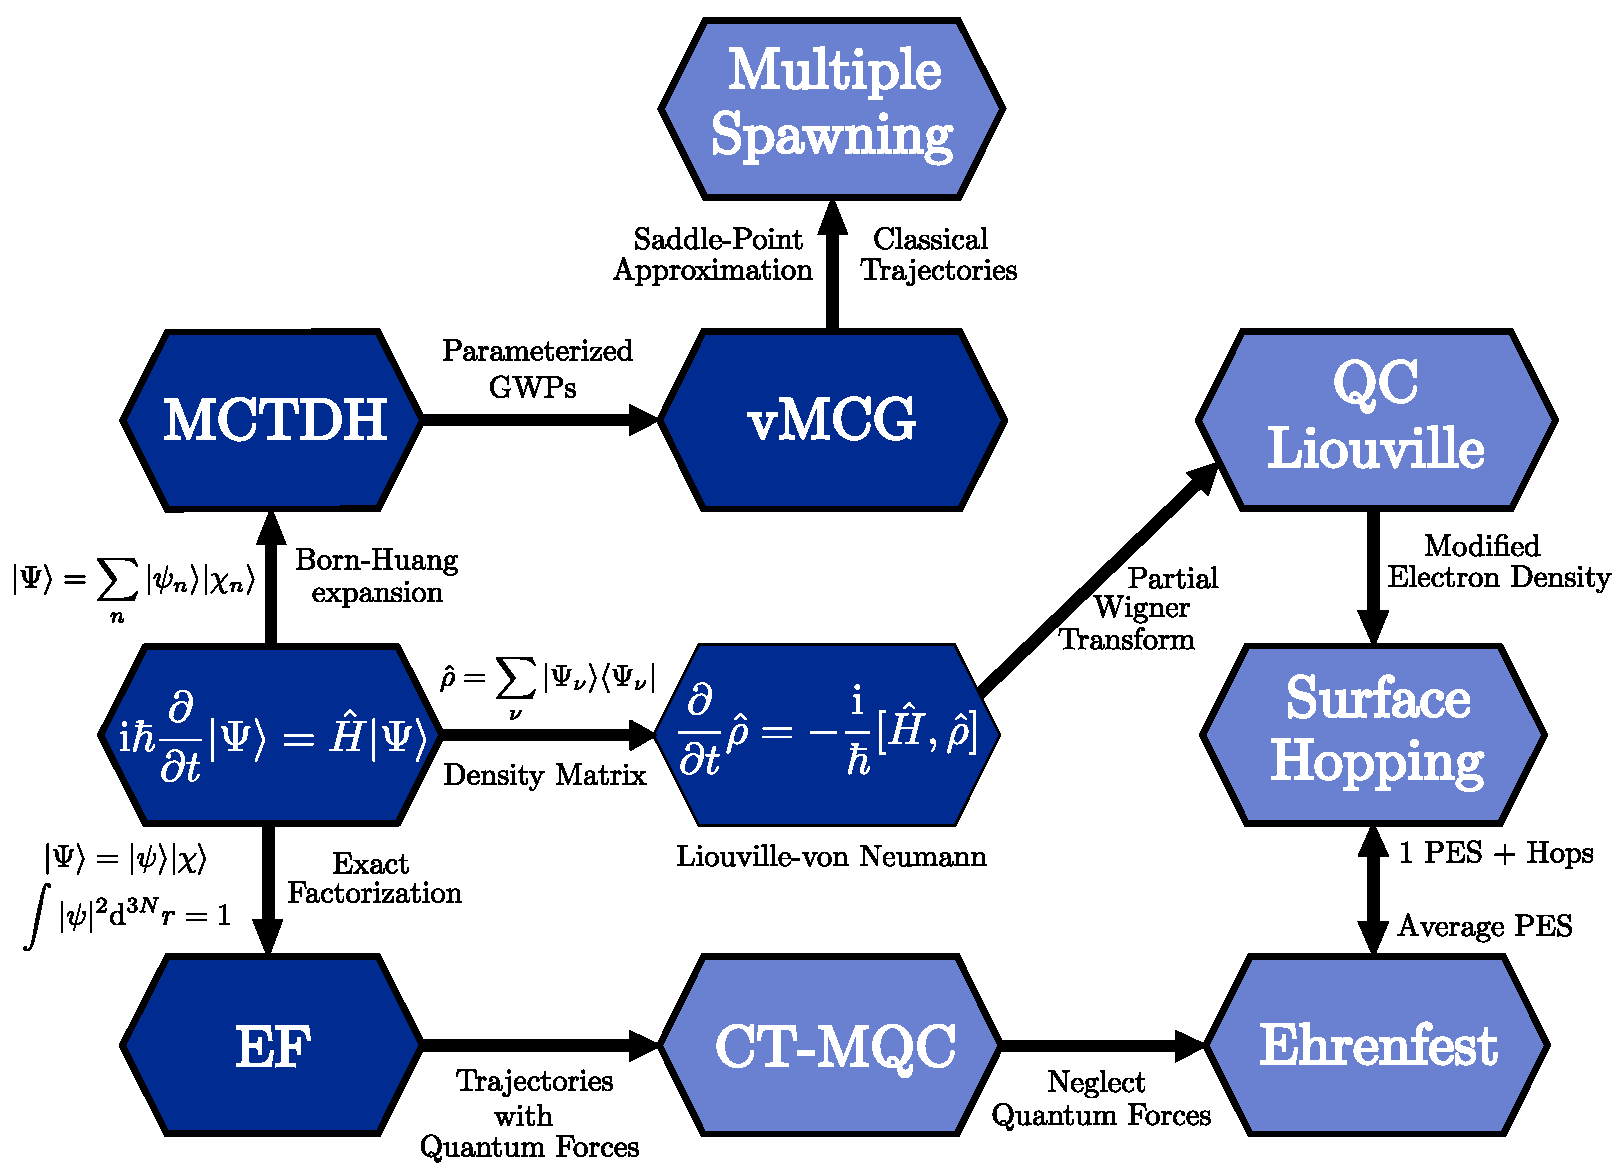
\includegraphics[width=15cm]{MQC_Algorithms.pdf}
\end{figure}




\subsection{Multiconfigurational Time-Dependent Hartree (MCTDH) Method}
The basis of deriving the MCTDH equations of motion is the Dirac-Frenkel variational principle. Applying it to the time dependent Schrödinger equation leads to
\begin{equation}
\langle\delta\Psi(t)|\hat{H}-\mathrm{i}\hbar\frac{\partial}{\partial t}|\Psi(t)\rangle = 0
\end{equation}

\subsection{Variational Multiconfigurational Gaussian Method (vMCG)}

\subsection{Ab Initio Multiple Spawning (AIMS)}

\subsection{Exact Factorization of the TDSE}

\subsection{Coupled-Trajectory Mixed Quantum-Classical Algorithm (CT-MQC)}

\subsection{Mean-Field Ehrenfest Dynamics}

\subsection{Trajectory Surface Hopping}

\subsection{Mixed Quantum-Classical Liouville Equation (QCLE)}












\newpage
\section{Path Integral Molecular Dynamics (PIMD)}
\url{https://www.youtube.com/watch?v=-Lnflp7JsxM}


\subsection{Derivation of the Path Integral}
Der Zeitentwicklungsoperator oder Propagator $\hat{U}(t)$ kann nicht nur auf die Eigenzustände des Hamiltonoperators, sondern auch auf die Eigenzustände des Ortsoperators angewendet werden:
\begin{equation}
|x'\rangle = \hat{U}(t)|x\rangle =\exp\Big(\frac{-i\hat{H}t}{\hbar}\Big)|x\rangle
\end{equation}
Die zugehörigen Matrixelemente sind dann gegeben durch
\begin{equation}
U(x,x';t)=\langle x'|e^{-\mathrm{i}\hat{H}t/\hbar}|x\rangle
\end{equation}
Wenn die Eigenzustände der Schrödingergleichung $|\Psi(t)$ auf die Basis der Ortszustände projiziert werden, ergibt sich:
\begin{align}
\langle x'|\Psi(t)\rangle &= \Psi(x',t) = \langle x'|e^{-\mathrm{i}\hat{H}t/\hbar}|\Psi(0)\rangle = \int\mathrm{d}x\langle x'|e^{-\mathrm{i}\hat{H}t/\hbar}|x\rangle\langle x|\Psi(0)\rangle\\
&= \int\mathrm{d}x\langle x'|e^{-\mathrm{i}\hat{H}t/\hbar}|x\rangle\Psi(x,0) = \int\mathrm{d}x U(x,x';t)\Psi(x,0)
\end{align}
Es besteht ein Zusammenhang zwischen dem Propagator $\hat{U}(t)$ und der kanonischen Dichtematrix $\hat{\rho}(\beta)=\exp(-\beta\hat{H})$. Gleichsetzen liefert:
\begin{equation}
e^{-\beta\hat{H}}=e^{-\mathrm{i}\hat{H}t/\hbar}\quad\Rightarrow\quad t=-\mathrm{i}\beta\hbar\quad\mathrm{und}\quad\beta=\frac{\mathrm{i}t}{\hbar}
\end{equation}
Daraus folgt direkt:
\begin{equation}
\hat{U}(-\mathrm{i}\beta\hbar) = \hat{\rho}(\beta)\qquad\mathrm{und}\qquad\hat{\rho}(\mathrm{i}t/\hbar) = \hat{U}(t)
\end{equation}
Im Folgenden soll das Pfadintegral für den kanonischen Dichteoperator hergeleitet werden, um daraus dann das Pfadintegral für den Propagator leichter bestimmen zu können. Zuerst wird der Dichteoperator in der Basis der Ortszustände geschrieben:
\begin{equation}
\rho(x,x';\beta) = \langle x'|e^{-\beta\hat{H}}|x\rangle
\end{equation}
Da der Hamitonian im kanonischen Dichteoperator aus den Operatoren der kinetischen und potentiellen Energie zusammengesetzt ist, die nicht miteinander kommutieren, kann keine einfache Zerlegung durchgeführt werden:
\begin{equation}
e^{-\beta\hat{H}}=e^{-\beta(\hat{T}+\hat{V})}\neq e^{-\beta\hat{T}}e^{-\beta\hat{V}}
\end{equation}
Stattdessen muss in diesem Fall das Trotter-Theorem angewendet werden:
\begin{equation}
e^{-\beta(\hat{T}+\hat{V})}=\lim_{P\to\infty}\bigg[\exp\Big(\frac{-\beta\hat{V}}{2P}\Big)\exp\Big(\frac{-\beta\hat{T}}{P}\Big)\exp\Big(\frac{-\beta\hat{V}}{2P}\Big)\bigg]^P
\end{equation}


\subsection{Ring Polymer Molecular Dynamics (RPMD)}

\subsection{Centroid Molecular Dynamics (CMD)}













\newpage
\section{Hierarchical Equations of Motion (HEOM)}

\subsection{The Path Integral in Configuration Space}
The time-dependent Schrödinger equation is not the only way to solve the dynamic time evolution of quantum states. If we apply the time evolution operator $\hat{U}(t_N,t_0)$ on a spacial state $x_0$ we get the time evolution of this state from $t_0$ to $t_N$:
\begin{equation}
|x_N\rangle = \hat{U}(t_N,t_0)|x_0\rangle =\exp\Big(\frac{-i\hat{H}(t_N-t_0)}{\hbar}\Big)|x_0\rangle
\end{equation}
Now we use the fact that the time evolution operator can be decomposed into products of operators if the time interval $[t_0,t_N]$ is sliced into $N$ pieces of length $\Delta t=(t_N-t_0)/N$. The corresponding matrix elements then read:
\begin{equation}
\langle x_N|\hat{U}(t_N,t_0)|x_0\rangle = \langle x_N|\hat{U}(t_N,t_{N-1})\hat{U}(t_{N-1},t_{N-2})\cdots\hat{U}(t_2,t_1)\hat{U}(t_1,t_0)|x_0\rangle
\end{equation}
Now the identity operator can be inserted $N-1$ times to obtain
\begin{equation}
\langle x_N|\hat{U}(t_N,t_0)|x_0\rangle = \prod_{j=1}^{N-1}\bigg[\int\mathrm{d}x_j\bigg]\prod_{j=1}^{N}\underbrace{\langle x_j|\hat{U}(t_j,t_{j-1})|x_{j-1}\rangle}_{=\Theta_{j,j-1}}\label{Time evolution product operators}
\end{equation}
Now we assume that the Hamiltonian is of the form $\hat{H}=T(\hat{p})+V(\hat{x})$ and that the time evolution operator can be decomposed into
\begin{equation}
\exp(-\mathrm{i}\hat{H}\Delta t/\hbar) \approx \exp(-\mathrm{i}V(\hat{x})\Delta t/\hbar)\exp(-\mathrm{i}T(\hat{p})\Delta t/\hbar)
\end{equation}
This is only approximately true because $T$ and $V$ are operators so that the Trotter theorem must be applied in a strict derivation. However, the difference is small in most cases. Now we take one matrix element from \eqref{Time evolution product operators} and evaluate the integral:
\begin{align}
\Theta_{j,j-1} &= \langle x_{j}|\hat{U}(t_j,t_{j-1})|x_{j-1}\rangle\\
&= \langle x_j|\exp(-\mathrm{i}V(\hat{x})\Delta t/\hbar)\exp(-\mathrm{i}T(\hat{p})\Delta t/\hbar)|x_{j-1}\rangle\\
&= \int\mathrm{d}x \langle x_j|\exp(-\mathrm{i}\hat{V}\Delta t/\hbar)|x\rangle\langle x|\exp(-\mathrm{i}\hat{T}\Delta t\hbar)|x_{j-1}\rangle\\
&= \int\mathrm{d}x\langle x_j|\exp(-\mathrm{i}\hat{V}\Delta t/\hbar)|x\rangle\langle x|\int\mathrm{d}p_j|p_j\rangle\langle p_j|\exp(-\mathrm{i}\hat{T}\Delta t/\hbar)\int\mathrm{d}p|p\rangle\langle p|x_{j-1}\rangle\\
&= \int\mathrm{d}x\int\mathrm{d}p_j\int\mathrm{d}p\langle x_j|\exp(-\mathrm{i}\hat{V}\Delta t/\hbar)|x\rangle\langle x|p_j\rangle\langle p_j|\exp(-\mathrm{i}\hat{T}\Delta t/\hbar)|p\rangle\langle p|x_{j-1}\rangle\\
&=\int\mathrm{d}x\int\mathrm{d}p_j\int\mathrm{d}p\exp(-\mathrm{i}\hat{V}(x_j)\Delta t/\hbar)\delta(x-x_j)\exp(\mathrm{i}p_j x/\hbar)\frac{1}{\sqrt{2\pi\hbar}}\exp(-\mathrm{i}\hat{T}(p_j)\Delta t/\hbar)\delta(p-p_j)\exp(\mathrm{i}x_{j-1}p/\hbar)\frac{1}{\sqrt{2\pi\hbar}}\notag\\
&= \int\exp(-\mathrm{i}V(x_j)\Delta t/\hbar)\exp(-\mathrm{i}T(p_j)\Delta t/\hbar)\int\exp(\mathrm{i}p_j x/\hbar)\frac{1}{\sqrt{2\pi\hbar}}\delta(x-x_j)\mathrm{d}x\int\exp(\mathrm{i}x_{j-1}p/\hbar)\frac{1}{\sqrt{2\pi\hbar}}\delta(p-p_j)\mathrm{d}p\mathrm{d}p_j\notag\\
&= \int\frac{\mathrm{d}p_j}{2\pi\hbar}\exp(-\mathrm{i}V(x_j)\Delta t/\hbar)\exp(\mathrm{i}p_j(x_j-x_{j-1})/\hbar)\exp(-\mathrm{i}T(p_j)\Delta t/\hbar)
\end{align}
With this expression we can rewrite the whole time evolution matrix element as
\begin{align}
&\prod_{j=1}^{N-1}\bigg[\int\mathrm{d}x_j\bigg]\prod_{j=1}^{N}\bigg[\int\frac{\mathrm{d}p_j}{2\pi\hbar}\bigg]\exp\bigg(\frac{\mathrm{i}}{\hbar}\sum_{j=1}^{N}\Big[p_j(x_j-x_{j-1})-\Delta t\big(T(p_j)+V(x_j)\big)\Big]\bigg)\\
=& \prod_{j=1}^{N-1}\bigg[\int\mathrm{d}x_j\bigg]\prod_{j=1}^{N}\bigg[\int\frac{\mathrm{d}p_j}{2\pi\hbar}\bigg]\exp\bigg(\frac{\mathrm{i}}{\hbar}\sum_{j=1}^{N}\Big[\frac{\Delta t}{2m}\Big(p_j-\frac{x_j-x_{j-1}}{\Delta t}m\Big)^2+\frac{m}{2}\Delta t\Big(\frac{x_j-x_{j-1}}{\Delta t}\Big)^2-\Delta t V(x_j)\Big]\bigg)\\
=& \prod_{j=1}^{N-1}\bigg[\int\mathrm{d}x_j\bigg]\prod_{j=1}^{N}\bigg[\frac{1}{2\pi\hbar}\int_{-\infty}^{\infty}\exp\bigg(-\frac{\mathrm{i}}{\hbar}\frac{\Delta t}{2m}\Big(p_j-\frac{x_j-x_{j-1}}{\Delta t}m\Big)^2\bigg)\mathrm{d}p_j\bigg]\exp\bigg(\frac{\mathrm{i}}{\hbar}\sum_{j=1}^{N}\Big[\frac{m}{2}\Delta t\Big(\frac{x_j-x_{j-1}}{\Delta t}\Big)^2-\Delta tV(x_j)\Big]\bigg)\notag\\
=& \prod_{j=1}^{N-1}\bigg[\int\mathrm{d}x_j\bigg]\bigg(\frac{1}{\sqrt{2\pi\hbar\mathrm{i}\Delta t/m}}\bigg)^N\exp\bigg(\frac{\mathrm{i}}{\hbar}\Delta t\sum_{j=1}^{N}\Big[\frac{m}{2}\Big(\frac{x_j-x_{j-1}}{\Delta t}\Big)^2-V(x_j)\Big]\bigg)\\
=& \frac{1}{\sqrt{2\pi\hbar\mathrm{i}\Delta t/m}}\prod_{j=1}^{N-1}\bigg[\int\frac{\mathrm{d}x_j}{\sqrt{2\pi\hbar\mathrm{i}\Delta t/m}}\bigg]\exp\bigg(\frac{\mathrm{i}}{\hbar}\Delta t\sum_{j=1}^{N}\Big[\frac{m}{2}\Big(\frac{x_j-x_{j-1}}{\Delta t}\Big)^2-V(x_j)\Big]\bigg)
\end{align}
If we now take the continuum limit, $\Delta t\to 0$, the sum in the exponent becomes an integral over time in the interval $[t_0,t_N]$:
\begin{align}
&\int\exp\bigg(\frac{\mathrm{i}}{\hbar}\int_{t_0}^{t_N}\frac{1}{2}m\dot{x}^2(t)-V(x)\mathrm{d}t\bigg)\mathcal{D}x\\
=& \int\exp\bigg(\frac{\mathrm{i}}{\hbar}\int_{t_0}^{t_N}\mathcal{L}(x,\dot{x},t)\mathrm{d}t\bigg)\mathcal{D}x
\end{align}






\subsection{Path Integral Representation of the Reduced Density Matrix}



\subsection{Feynman-Vernon Influence Functional}





The hierarchical equations of motion for a system in a harmonic Markovian bath are
\begin{equation}
\frac{\partial}{\partial t}\hat{\rho}_{n}=-i(\hat{H}_{A}+n\gamma)\hat{\rho}_{n}-\frac{1}{\hbar}\hat{V}^{\times}\hat{\rho}_{n+1}+\frac{in}{\hbar}\hat{\Theta}\hat{\rho}_{n-1}
\end{equation}
Another form is:
\begin{align}
\frac{\partial}{\partial t}\hat{\rho}_{n}(t) &= -(\mathrm{i}\hat{\mathcal{L}}+\gamma_n)\hat{\rho}_{n}(t)
\end{align}






\subsection{Example Calculations}
\url{https://www.ks.uiuc.edu/Research/phi/}
\begin{figure}[H]
	\centering
	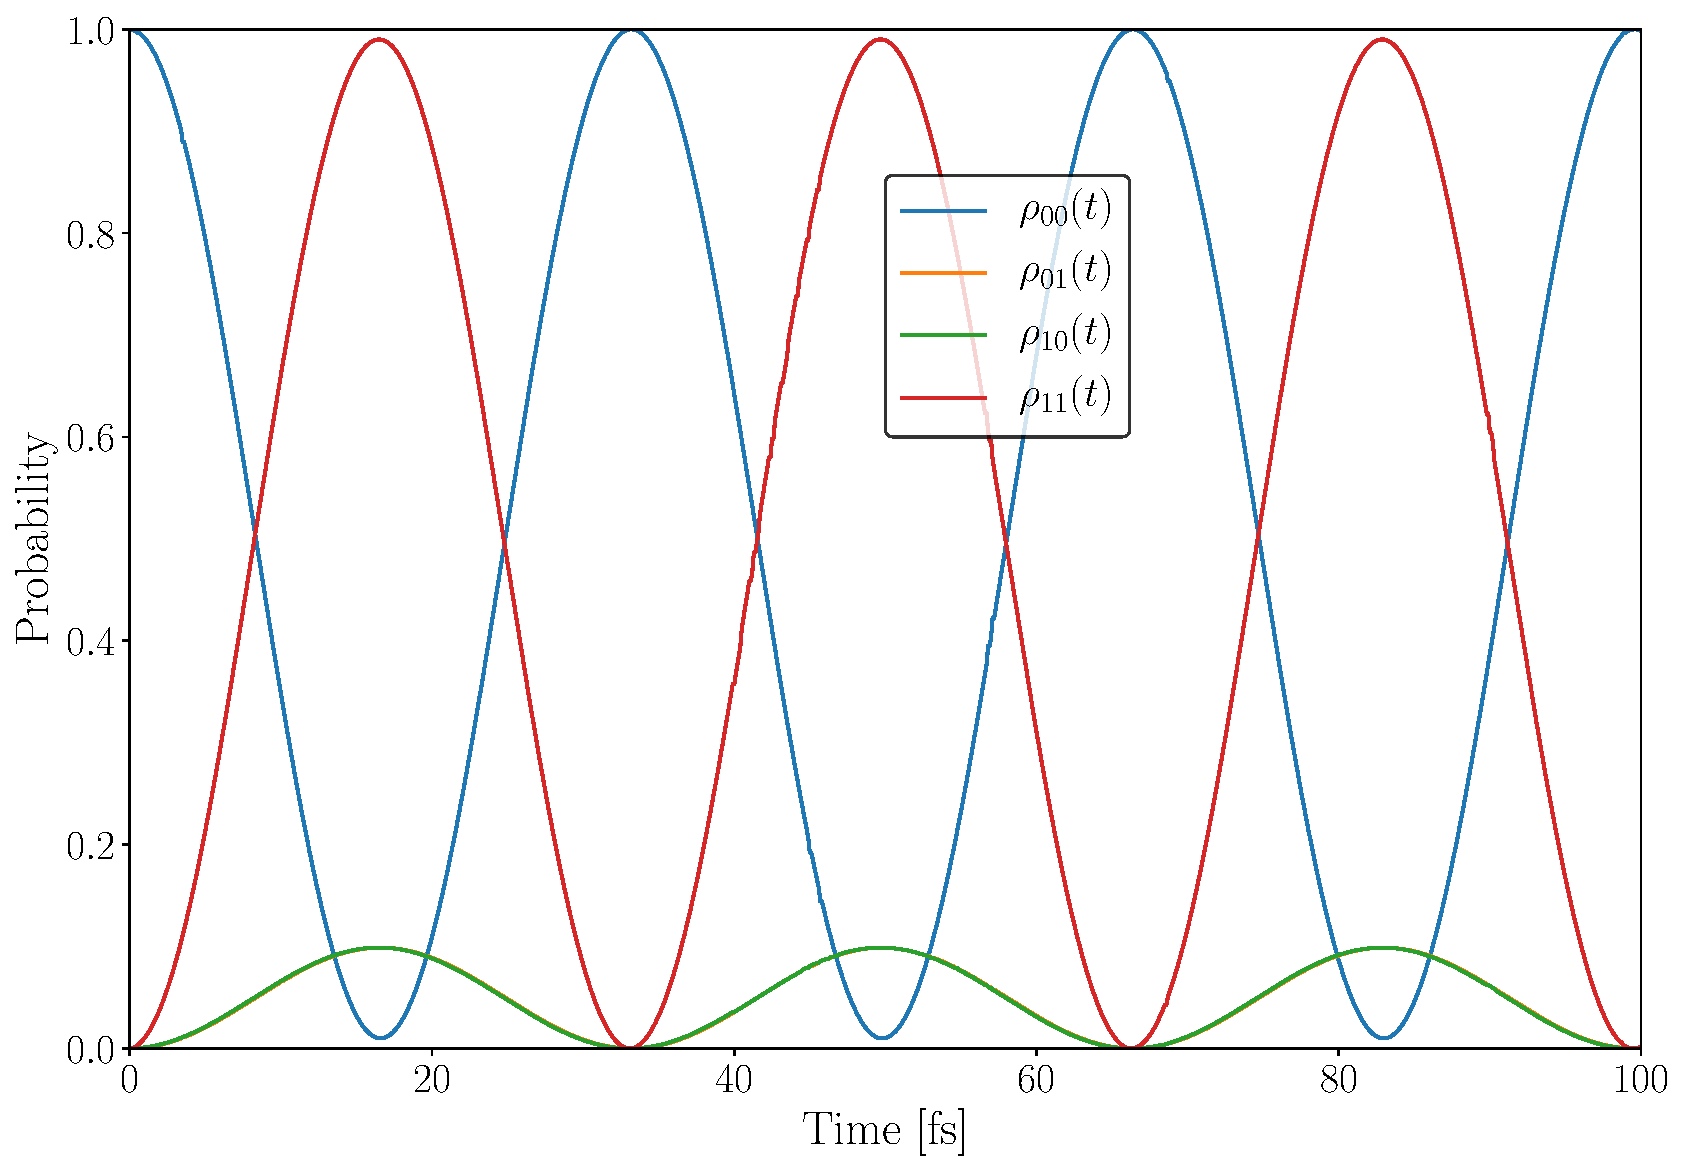
\includegraphics[width=15cm]{Special_Pair_1.pdf}
\end{figure}

























































\chapter{Quantum Optics}

\section{Weak Coupling Regime}
Lorentzian Shape of absorption spectra. Time-energy uncertainty.

\subsection{Fermi's Golden Rule}
In the fields of quantum optics and molecular simulations, often cases occur in which the time evolution of a system in the presence of a much larger thermal bath needs to be calculated. The Hamiltonian of the composite system is then given by
\begin{equation}
\hat{H}=\hat{H}_{\mathrm{S}}+\hat{H}_{\mathrm{R}}+\hat{H}_{\mathrm{SR}}
\end{equation}
Here $\hat{H}_{\mathrm{SR}}$ is the coupling of the system to the thermal bath or reservoir. If the coupling is assumed to be weak, the system-reservoir coupling can be viewed as a small perturbation to the Hamiltonian of the system and we can use time-dependent perturbation theory to compute specific properties of the time evolution of the system. To derive the corresponding equations, one starts with the time-dependent Schrödinger equation
\begin{equation}
\mathrm{i}\hbar\frac{\partial}{\partial t}|\Psi(t)\rangle = (\hat{H}_{\mathrm{S}}+\hat{H}_{\mathrm{SR}})|\Psi(t)\rangle\label{Total_TDSE}
\end{equation}
The Schrödinger equation for the system only will be denoted as
\begin{equation}
\mathrm{i}\hbar\frac{\partial}{\partial t}|\Psi_{\mathrm{S}}(t)\rangle = \hat{H}_{\mathrm{S}}|\Psi_{\mathrm{S}}(t)\rangle
\end{equation}
Now we follow the usual separation of the Schrödinger equation into time- and spatially-dependent parts and write down the time-independent Schrödinger equation for the system Hamiltonian:
\begin{equation}
\hat{H}_{\mathrm{S}}|\phi_{\nu}\rangle = E_{\nu}|\phi_{\nu}\rangle
\end{equation}
Given some initial conditions, the general solution for the time-dependent Schrödinger equation at time $t=0$ can be written as
\begin{equation}
|\Psi_{\mathrm{S}}(0)\rangle = \sum_{\nu=0}^{\infty}a_{\nu}(t)|\phi_{\nu}\rangle
\end{equation}
The general solution at an arbitrary time $t$ can be calculated by applying the unitary time evolution operator $\hat{U}_{\mathrm{S}}(t)$ onto the state $|\Psi_{\mathrm{S}}(0)\rangle$:
\begin{equation}
|\Psi_{\mathrm{S}}(t)\rangle = \hat{U}_{\mathrm{S}}(t)|\Psi_{\mathrm{S}}(0)\rangle = \exp(-\mathrm{i}\hat{H}_{\mathrm{S}}t/\hbar)\sum_{\nu=0}^{\infty}a_{\nu}(t)|\phi_{\nu}\rangle\label{TDSE_Solution}
\end{equation}
Since the eigenstates $\phi_{\nu}$ of the system Hamiltonian $\hat{H}_{\mathrm{S}}$ form an orthonormal basis (ONB), it ist possible to also expand the total wavefunction $|\Psi(t)\rangle$ in this basis. Plugging in equation \eqref{TDSE_Solution} into equation \eqref{Total_TDSE} yields
\begin{align}
\mathrm{i}\hbar\frac{\partial}{\partial t}\Big(\hat{U}_{\mathrm{S}}(t)\sum_{\nu=0}^{\infty}a_{\nu}(t)|\phi_{\nu}\rangle\Big) &= (\hat{H}_{\mathrm{S}}+\hat{H}_{\mathrm{SR}})\hat{U}_{\mathrm{S}}(t)\sum_{\nu=0}^{\infty}a_{\nu}(t)|\phi_{\nu}\rangle\\
\mathrm{i}\hbar\sum_{\nu=0}^{\infty}\dot{a}_{\nu}(t)\hat{U}_{\mathrm{S}}(t)|\phi_{\nu}\rangle +\sum_{\nu=0}^{\infty}a_{\nu}(t)E_{\nu}\hat{U}_{\mathrm{S}}(t)|\phi_{\nu}\rangle &= \sum_{\nu=0}^{\infty}a_{\nu}(t)\hat{H}_{\mathrm{S}}\hat{U}_{\mathrm{S}}(t)|\phi_{\nu}\rangle +\sum_{\nu=0}^{\infty}a_{\nu}(t)\hat{H}_{\mathrm{SR}}\hat{U}_{\mathrm{S}}(t)|\phi_{\nu}\rangle\\
\sum_{\nu=0}^{\infty}a_{\nu}(t)\hat{H}_{\mathrm{SR}}\hat{U}_{\mathrm{S}}(t)|\phi_{\nu}\rangle &= \mathrm{i}\hbar\sum_{\nu=0}^{\infty}\dot{a}_{\nu}(t)\hat{U}_{\mathrm{S}}(t)|\phi_{\nu}\rangle\\
\sum_{\nu=0}^{\infty}a_{\nu}(t)\hat{U}_{\mathrm{S}}^{\dagger}(t)\hat{U}_{\mathrm{S}}(t)\langle\phi_{\mu}|\hat{H}_{\mathrm{SR}}|\phi_{\nu}\rangle &= \mathrm{i}\hbar\sum_{\nu=0}^{\infty}\dot{a}_{\nu}(t)\langle\phi_{\mu}|\hat{U}_{\mathrm{S}}^{\dagger}(t)\hat{U}_{\mathrm{S}}(t)|\phi_{\nu}\rangle\\
\dot{a}_{\nu}(t) &= \frac{1}{\mathrm{i}\hbar}\sum_{\nu=0}^{\infty}V_{\mu\nu}a_{\nu}(t)\exp(\mathrm{i}\omega_{\mu\nu}t)
\end{align}
with $V_{\mu\nu}=\langle\phi_{\mu}|\hat{H}_{\mathrm{SR}}|\phi_{\nu}\rangle$ and $\omega_{\mu\nu}=(E_{\mu}-E_{\nu})/\hbar$.



















\subsection{Quantization of the Electromagnetic Field}
\url{https://en.wikipedia.org/wiki/Quantization_of_the_electromagnetic_field}

\subsection{Spontaneous Emission}

\subsection{Wigner-Weisskopf Approach}



\subsection{Selection Rules, Transition Dipole Moments and Symmetry Aspects}
\begin{itemize}
	\item Symmetry suppressed spontaneous emission in chlorophyll molecules
	\item Irreducible representations and optical transitions in transition metal complexes
	\item Symmetry deduced selection rules in hydrogen atom and harmonic oscillator
	\item Circular dichroism spectroscopy and irreducible representations
	\item Symmetry aspects of vibrational transitions for IR spectra
\end{itemize}









\section{Jaynes-Cummings Model}

The full Hamiltonian in second quantization of a system composed of an electromagnetic field with $k$ modes interacting with a two-level atom is given by
\begin{equation}
\hat{H}=\sum_{j}E_{j}\hat{b}_{j}^{\dagger}\hat{b}_{j} +\sum_{k}\hbar\omega_{k}\hat{a}_{k}^{\dagger}\hat{a}_{k} +\hbar\sum_{i,j,k}\hat{b}_{i}^{\dagger}\hat{b}_{j}\big(g_{ijk}\hat{a}_{k}+g_{ijk}^{*}\hat{a}_{k}^{\dagger}\big)
\end{equation}

Fock states and coherent states. Rabi Cycle. Resonance Fluorescence. Stimulated Emission.\\
\url{https://en.wikipedia.org/wiki/Cavity_quantum_electrodynamics}\\
\url{https://en.wikipedia.org/wiki/Rabi_cycle}\\
\url{https://en.wikipedia.org/wiki/Vacuum_Rabi_oscillation}\\
\url{https://www.youtube.com/watch?v=zEAwL9GAPCo}\\
\url{https://github.com/jrjohansson/qutip-lectures/blob/master/Lecture-10-cQED-dispersive-regime.ipynb}


\subsection{Rotating Wave Approximation}
\url{https://en.wikipedia.org/wiki/Rotating_wave_approximation}\\

\subsection{AC Stark Shift}

\subsection{Stimulated and Spontaneous Emission}
\url{https://en.wikipedia.org/wiki/Quantum_efficiency}\\
\url{https://en.wikipedia.org/wiki/Quantum_yield}\\
\url{https://en.wikipedia.org/wiki/Spontaneous_emission}\\
\url{http://www.mikomma.de/fh/hydrod/emission/emission.htm}
Kann man ein Molekül und die Molekül-Photon-Wechselwirkung komplett quantenelektrodynamisch berechnen?\\
Führen magnetische Wechselfelder zu einer zeitabhängigen Aufspaltung von Spin-Multipletts?\\
Version des Jaynes-Cummings-Modells für magnetische Wechselfelder?\\
Lässt sich die Molekül-Photon-Wechselwirkung in Quanten-Mastergleichungen integrieren?\\
Ist eine quantenelektrodynamische Berechnung von NMR- und EPR-Energieniveaus und Interaktion mit Photonen möglich?\\

\subsection{Creation of Entangled Bell States}

\subsection{Dicke Model and Superradiance}





\section{Quantum Optical Dynamics with Dissipation}

\subsection{Quantum Stochastic Differential Equations}
\url{https://en.wikipedia.org/wiki/Quantum_stochastic_calculus}\\
\url{https://www.amazon.de/Quantum-Noise-Non-Markovian-Applications-Synergetics/dp/3540223010}\\
\url{https://www.youtube.com/watch?v=ThsSubLaKeA&t=3021s}\\

\subsection{Quantum Optical Master Equation in Lindblad Form}
The Lindblad quantum master equation in its most general form is given by
\begin{equation}
\frac{\partial}{\partial t}\hat{\rho}_{\mathrm{S}}(t) = -\frac{\mathrm{i}}{\hbar}\big[\hat{H}_{\mathrm{S}},\hat{\rho}_{\mathrm{S}}(t)\big]+\sum_{n,m=1}^{N^2-1}h_{nm}\Big(\hat{A}_{n}\hat{\rho}_{\mathrm{S}}(t)\hat{A}_{m}^{\dagger}-\frac{1}{2}\big\{\hat{A}_{m}^{\dagger}\hat{A}_{n},\hat{\rho}_{\mathrm{S}}(t)\big\}\Big)
\end{equation}
The Lindblad equation of Jaynes-Cummings type reads
\begin{equation}
\frac{\partial}{\partial t}\hat{\rho}_{\mathrm{S}}(t) = -\frac{\mathrm{i}}{\hbar}\big[\hat{H}_{\mathrm{S}},\hat{\rho}_{\mathrm{S}}(t)\big]+\gamma\sum_{j}\Big(\hat{A}_{j}\hat{\rho}_{\mathrm{S}}(t)\hat{A}_{j}^{\dagger}-\frac{1}{2}\big\{\hat{A}_{j}^{\dagger}\hat{A}_{j},\hat{\rho}_{\mathrm{S}}(t)\big\}\Big)
\end{equation}
\url{http://qutip.org/docs/latest/guide/dynamics/dynamics-master.html}
\begin{figure}[H]
	\centering
	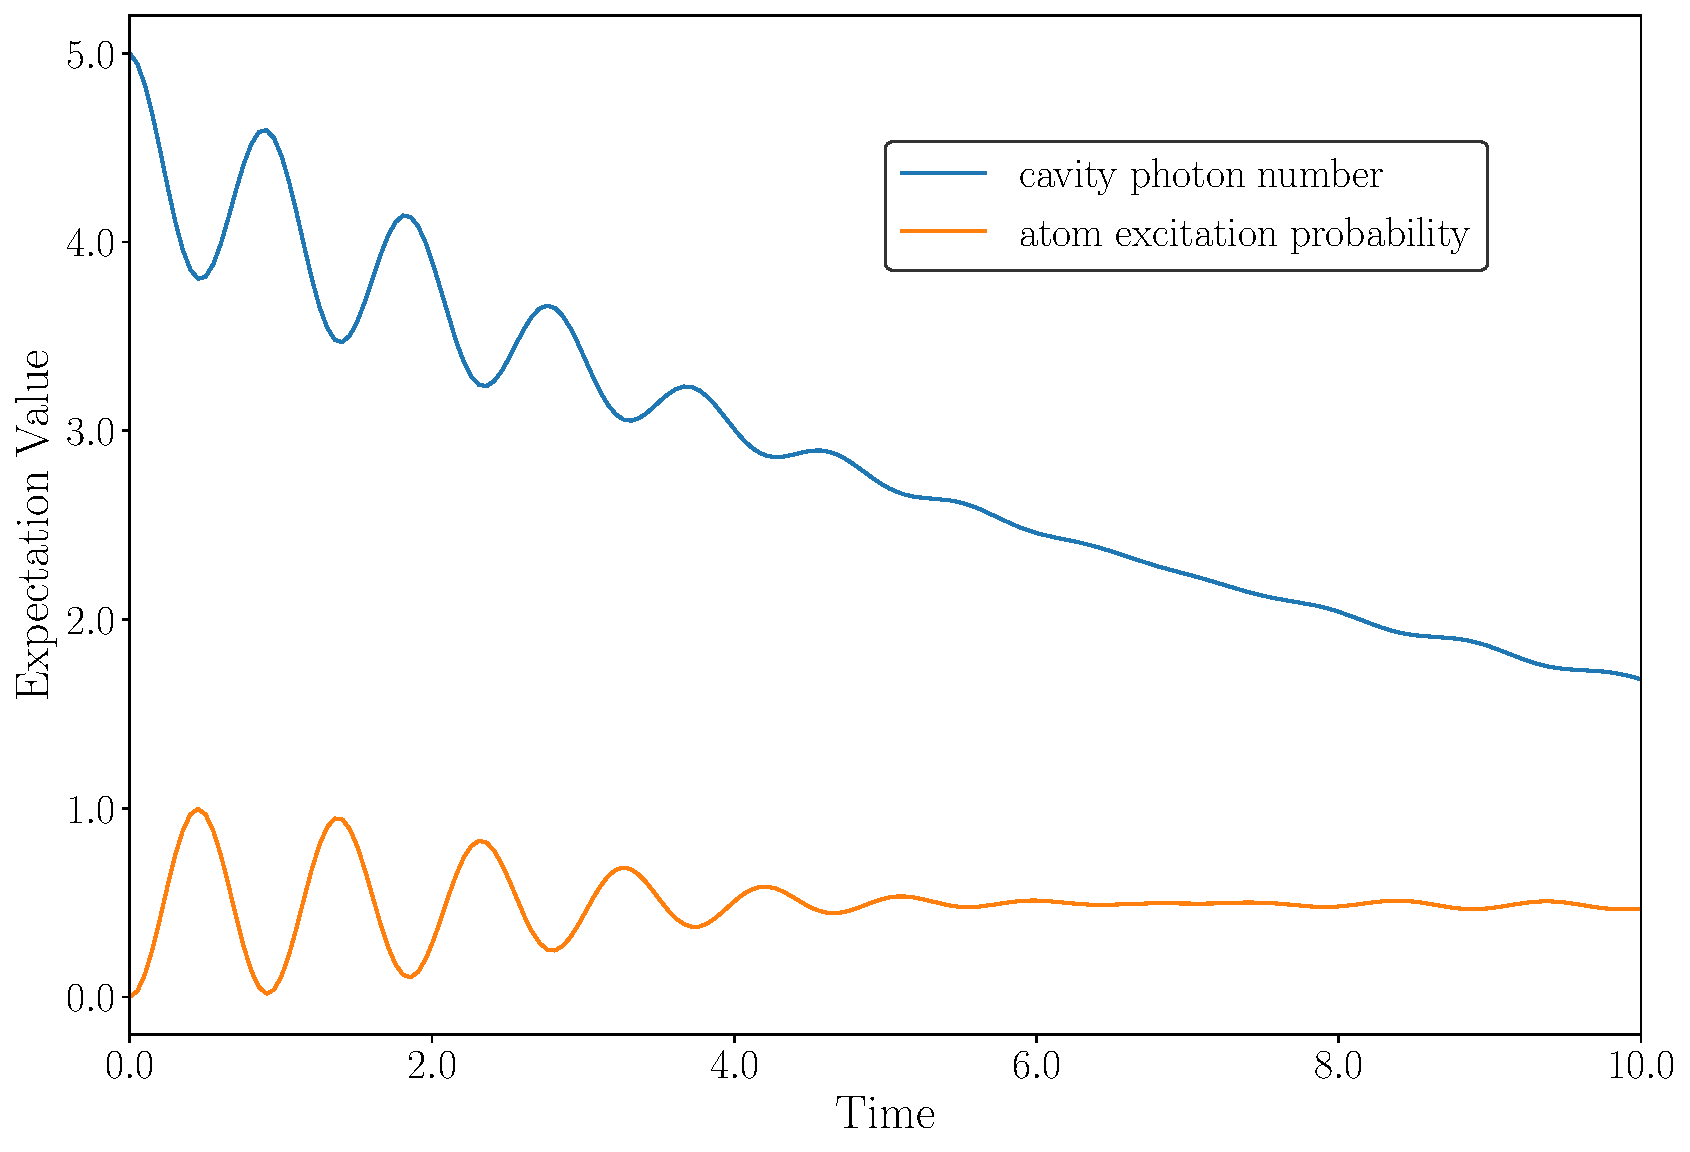
\includegraphics[width=14cm]{Jaynes-Cummings-Dynamics.pdf}
	\caption{Lindblad time evolution of a two-level atom in a one-mode cavity containing 5 initial photons}
\end{figure}


\subsection{Lindblad Equation for a Two-Level System with Decay}
\begin{equation}
\frac{\partial\hat{\rho}(t)}{\partial t}=-\frac{\mathrm{i}}{\hbar}\big[\hat{H},\hat{\rho}(t)\big]+\Gamma\Big(\hat{\sigma}^{-}\hat{\rho}(t)\hat{\sigma}^{+}-\frac{1}{2}\big\{\hat{\sigma}^{+}\hat{\sigma}^{-},\hat{\rho}(t)\big\}\Big)
\end{equation}

\subsection{Optical Bloch Equations}
\url{https://en.wikipedia.org/wiki/Maxwell%E2%80%93Bloch_equations#Derivation_from_cavity_quantum_electrodynamics}







\newpage
\section{Nuclear Spin Dynamics of an Ethanol Molecule}

\subsection{Nuclear Spin Hamiltonian}
\begin{equation}
\hat{H}_{\mathrm{Z}}=\displaystyle\sum_{i=1}^{N}\hat{H}_{\mathrm{Z},i}=\hbar\displaystyle\sum_{i=1}^{N}\omega_{i}^{0}\hat{I}_{iz}=-\frac{\hbar\gamma B_{0}}{2\pi}\displaystyle\sum_{i=1}^{N}(1+\delta_{i})\hat{I}_{iz}
\end{equation}
Since the Hamiltonian $\hat{H}_{\mathrm{Z}}$ does not act on the Hilbert space $\mathcal{H}_i$ of a single spin-1/2 system, but on the Hilbert space of 6 interacting spins $\mathcal{H}_1\otimes\mathcal{H}_2\otimes\mathcal{H}_3\otimes\mathcal{H}_4\otimes\mathcal{H}_5\otimes\mathcal{H}_6$, we have to take the tensor sum of the operators in order to construct the matrix reprsentation for the full space:
\begin{equation}
\op_{i=1}^{m}H_i = \sum_{i=1}^{m}\bigg(\bigotimes_{j=1}^{i-1}\mathbbm{1}_j\bigg)\otimes H_i\otimes\bigg(\bigotimes_{j=i+1}^{m}\mathbbm{1}_j\bigg)
\end{equation}
For example:
\begin{equation}
H_1\boxplus H_2\boxplus H_3 = H_1\otimes\mathbbm{1}_2\otimes\mathbbm{1}_3 + \mathbbm{1}_1\otimes H_2\otimes\mathbbm{1}_3 + \mathbbm{1}_1\otimes\mathbbm{1}_2\otimes H_3
\end{equation}

\subsection{Unitary Time Evolution}

\subsection{Dissipative Dynamics using the Redfield Equation}

\subsection{2D NMR Spectrum}
\url{https://en.wikipedia.org/wiki/Spin_echo}\\
\url{https://en.wikipedia.org/wiki/Relaxation_(NMR)#Microscopic_mechanisms}\\
\url{https://web.stanford.edu/class/rad226b/Lectures/}\\
\url{https://books.google.de/books?id=a3t_ysBNwD4C&pg=PA308&lpg=PA308&dq=von+neumann+equation+off+diagonal+elements&source=bl&ots=hqO1tAdJh4&sig=ACfU3U0YmRpyOJLkBl8ekPe9JToMjFXQsQ&hl=de&sa=X&ved=2ahUKEwiR0rPW0r3oAhWQO8AKHYCSCz8Q6AEwCXoECAoQAQ#v=onepage&q=von%20neumann%20equation%20off%20diagonal%20elements&f=false}


\section{2D Electronic Spectroscopy}

\section{2D Vibrational Spectroscopy}
\url{https://aip.scitation.org/doi/full/10.1063/1.5083966}\\
\url{https://en.wikipedia.org/wiki/Yoshitaka_Tanimura}



\section{Electronic Circular Dichroism}
Es kann eine Verbindung zwischen der optischen Aktivität eines Moleküls (bei Absorption zirkular polarisierten Lichts) und seinen quantenmechanischen Zuständen hergestellt werden. Bei Anregung aus dem Grundzustand $|\Psi_{0}\rangle$ in einen elektronisch angeregten Zustand $|\Psi_{\nu}\rangle$ entspricht der Imaginärteil des Skalarprodukts aus dem elektrischen ($\hat{\vec{\mu}}_{0\nu}$) und magnetischen ($\hat{\vec{m}}_{0\nu}$) Übergangsdipolmoment (TDM) der sogenannten Rotationsstärke $R_{0\nu}$:
\begin{equation}
R_{0\nu}=\Im\Big(\big\langle\Psi_{0}\big|\hat{\vec{\mu}}\big|\Psi_{\nu}\big\rangle\big\langle\Psi_{\nu}\big|\hat{\vec{m}}\big|\Psi_{0}\big\rangle\Big)
\end{equation}

\subsection{One-Photon CD Transitions}
\subsection{Two-Photon CD Transitions}


\section{Raman Transitions}





\section{Greenhouse Effect}

\subsection{Planck's Law}
\begin{figure}[H]
	\centering
	\begin{subfigure}[b]{0.53\textwidth}  
		\centering 
		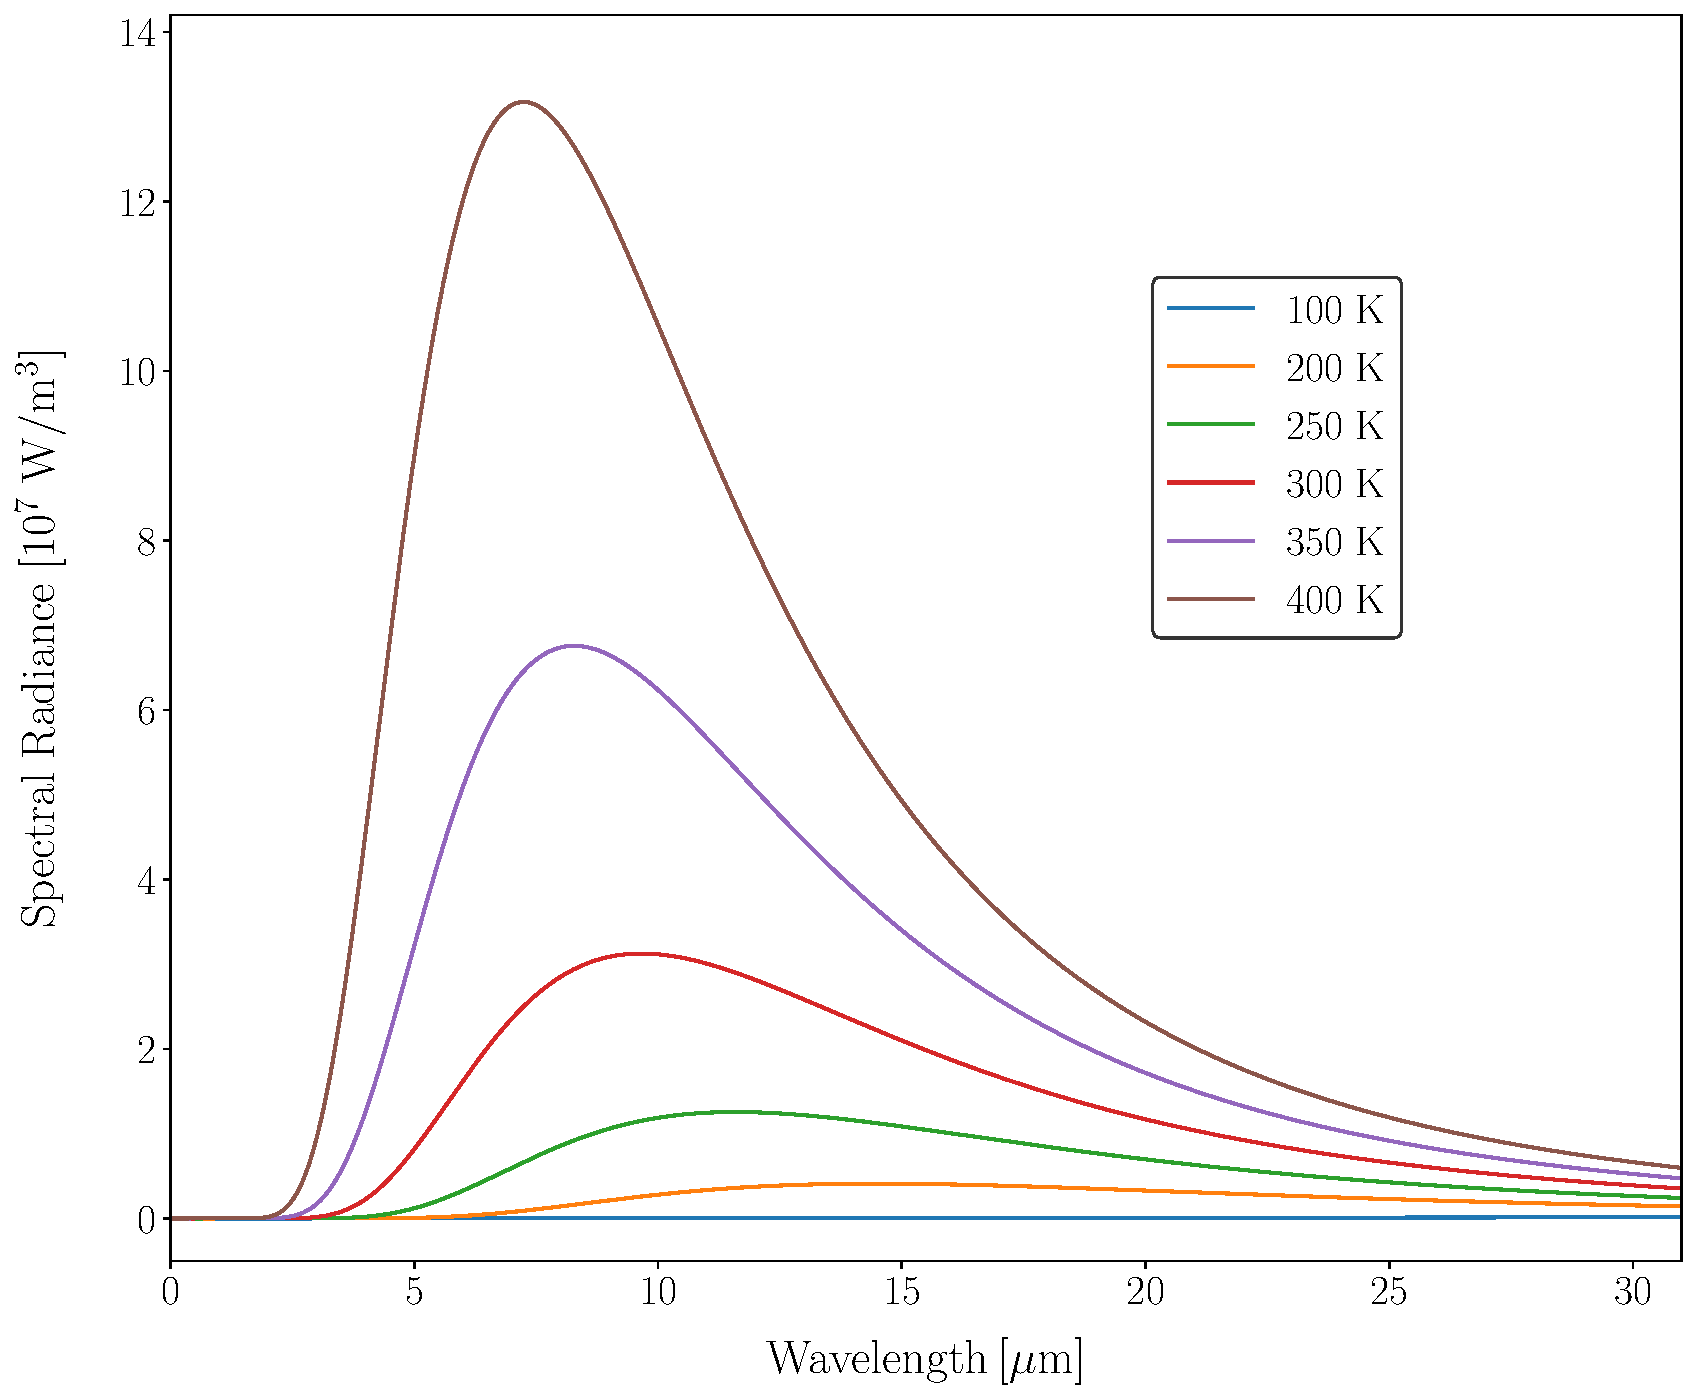
\includegraphics[width=\textwidth]{Planck-Strahlungsgesetz.pdf}  
	\end{subfigure}
	\hfill
	\begin{subfigure}[b]{0.43\textwidth}
		\centering
		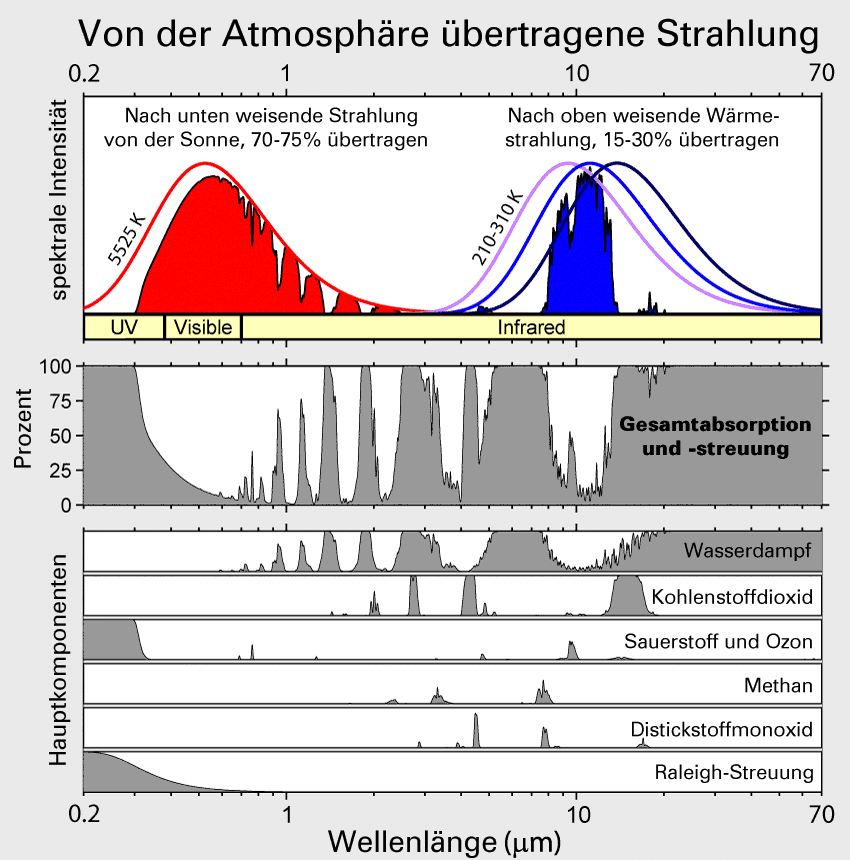
\includegraphics[width=\textwidth]{Atmospheric_Transmission.png}
	\end{subfigure}
\end{figure}
Planck's Law is given by:
\begin{equation}
B(\omega,T)=\frac{\hbar \omega^3}{4\pi^3 c^2}\frac{1}{\displaystyle\exp\Big(\frac{\hbar\omega}{k_{\mathrm{B}}T}\Big)-1}
\end{equation}




\subsection{Vibrational Spectra of Greenhouse Gases}

\subsection{Cross Sections for Absorption}

\subsection{Schwarzschild Equation}





\section{Trapped Ion Qubit Dynamics}




































\newpage
\chapter{Photosynthetic Light Reactions}





\begin{figure}[H]
	\centering
	\begin{subfigure}[b]{0.49\textwidth}  
		\centering 
		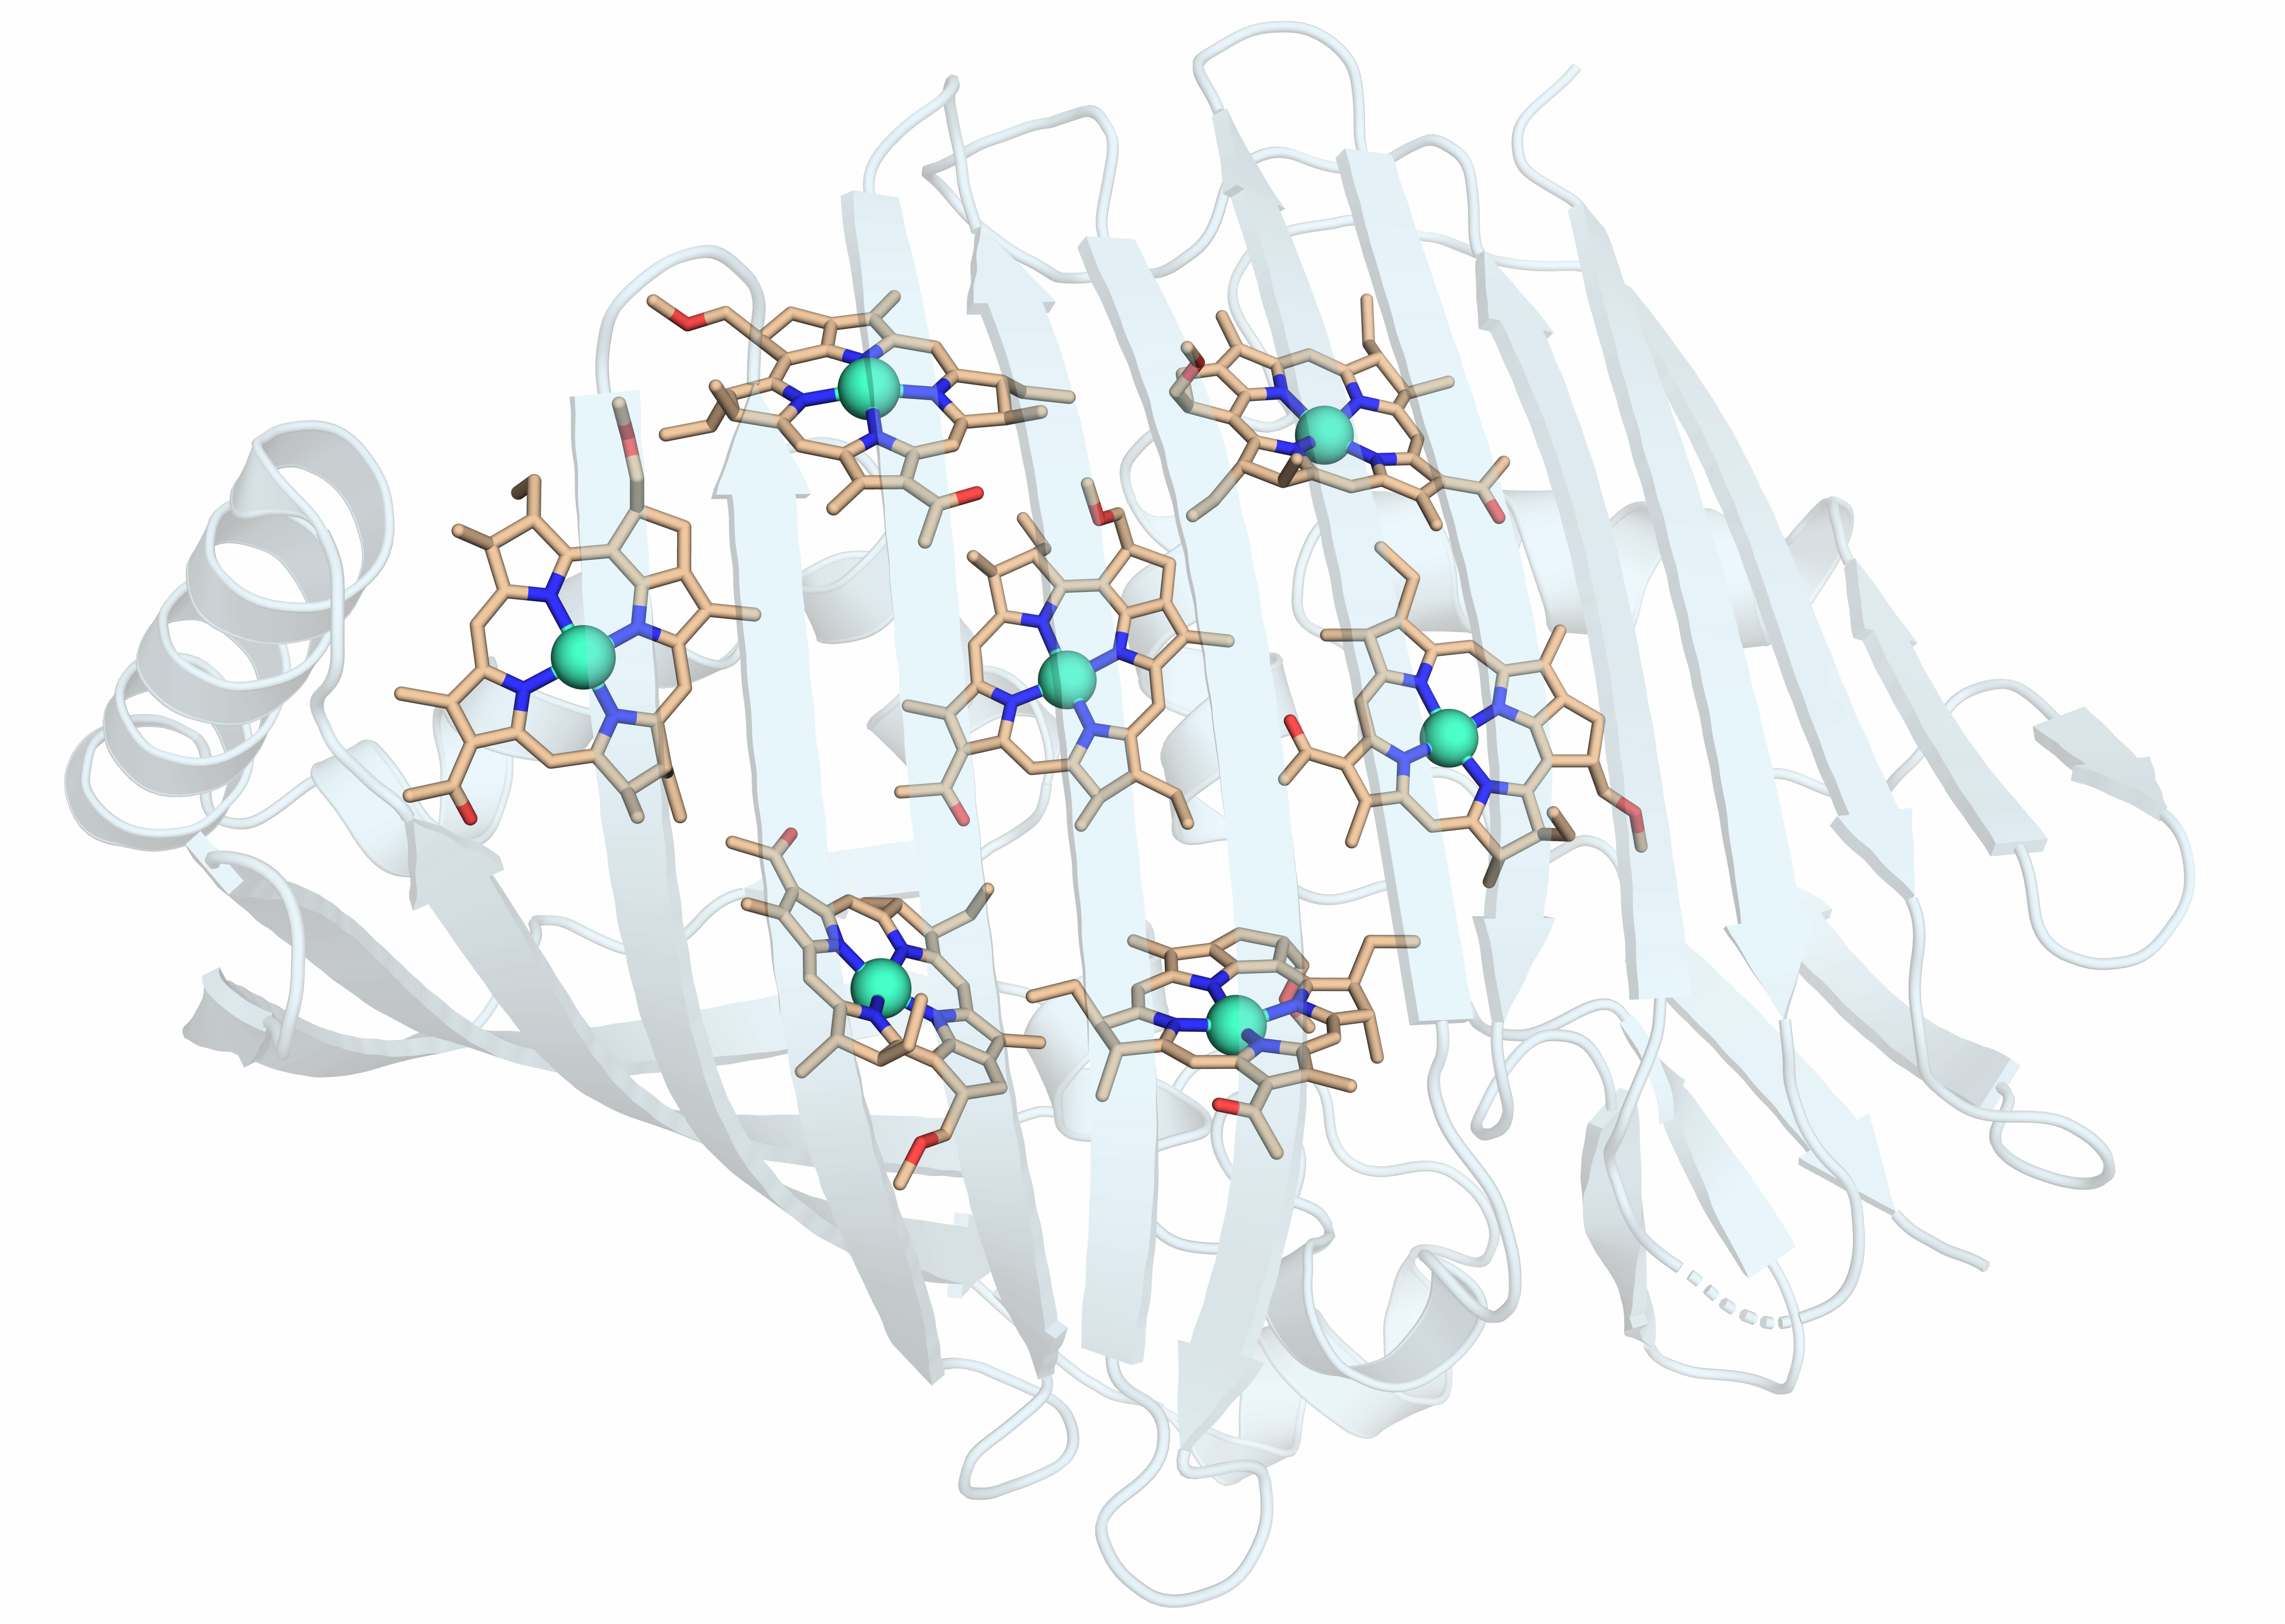
\includegraphics[width=\textwidth]{FMO.png}  
		\caption{The Fenna-Matthews-Olsen complex.}
	\end{subfigure}
	\hfill
	\begin{subfigure}[b]{0.49\textwidth}
		\centering
		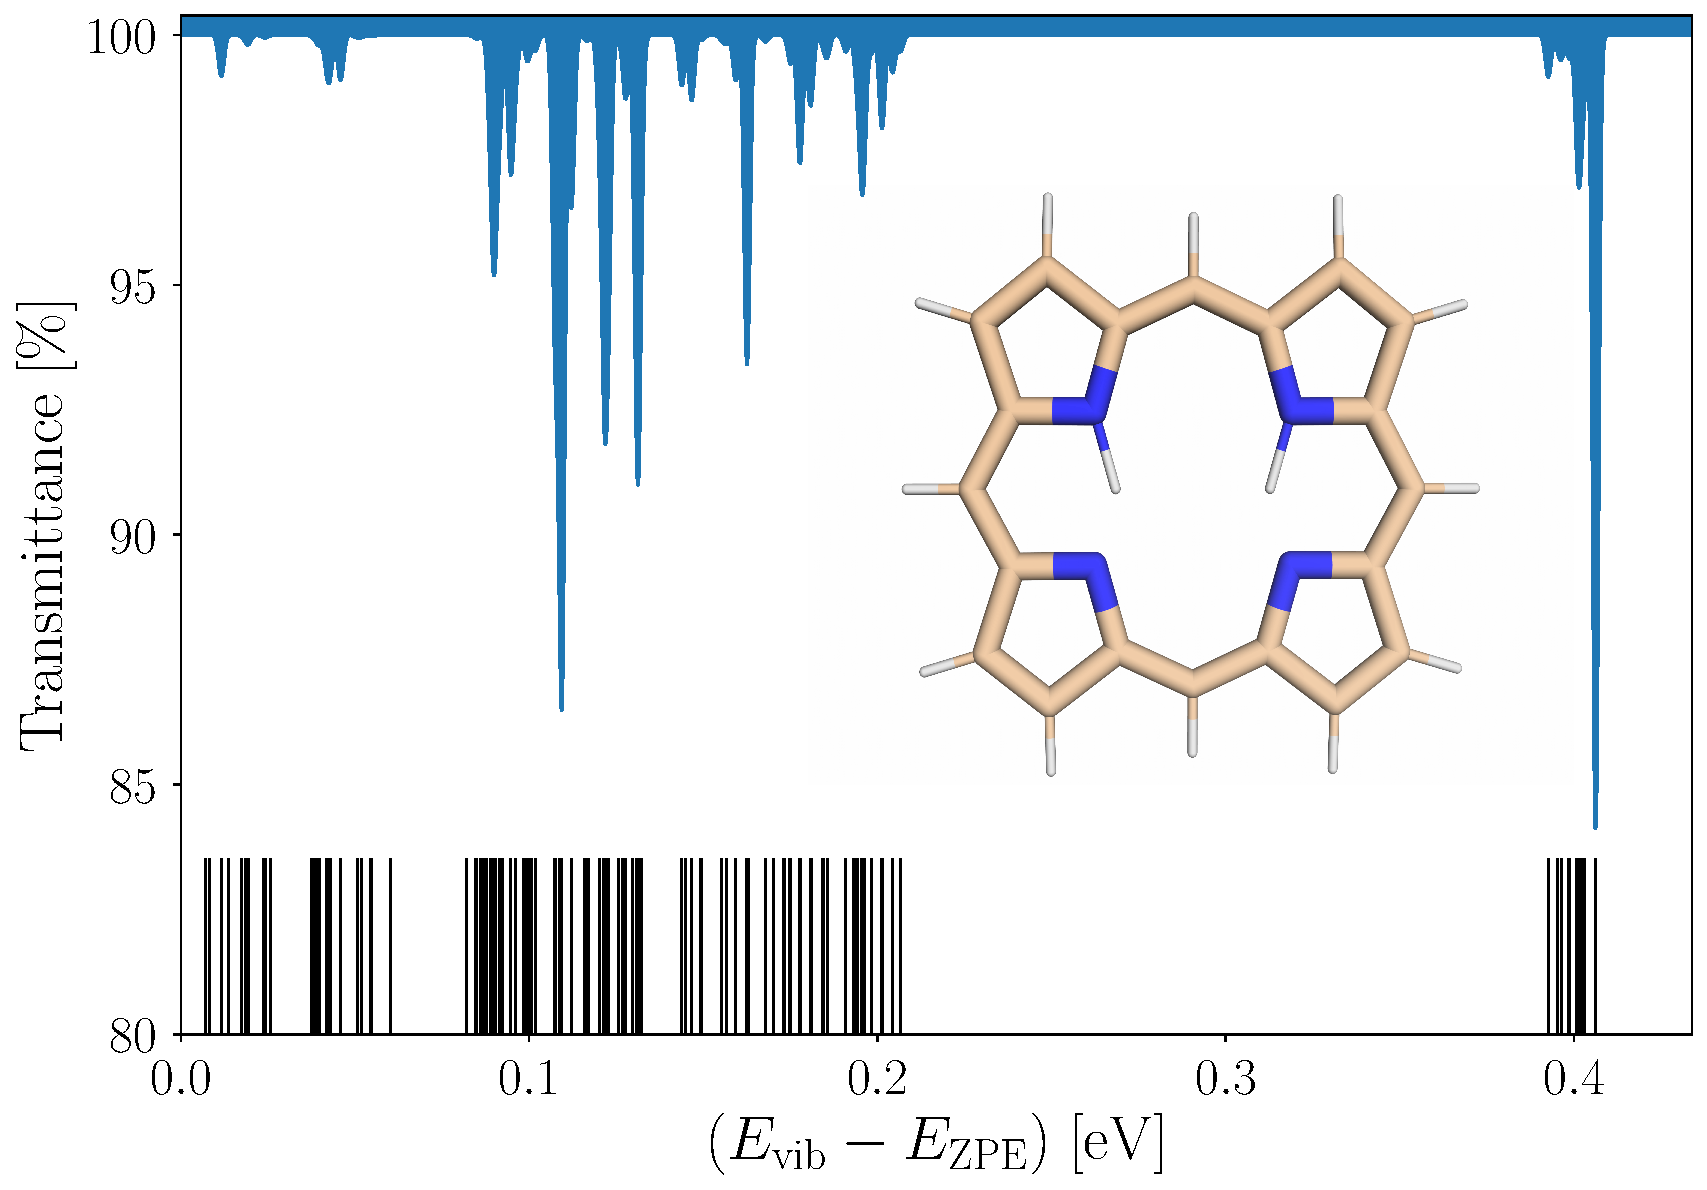
\includegraphics[width=\textwidth]{Porphyrin_IR.pdf}
		\caption{Infrared spectrum of Porphyrin calculated with ORCA.}
	\end{subfigure}
    \vskip\baselineskip
    \begin{subfigure}[b]{0.48\textwidth}
    	\centering
    	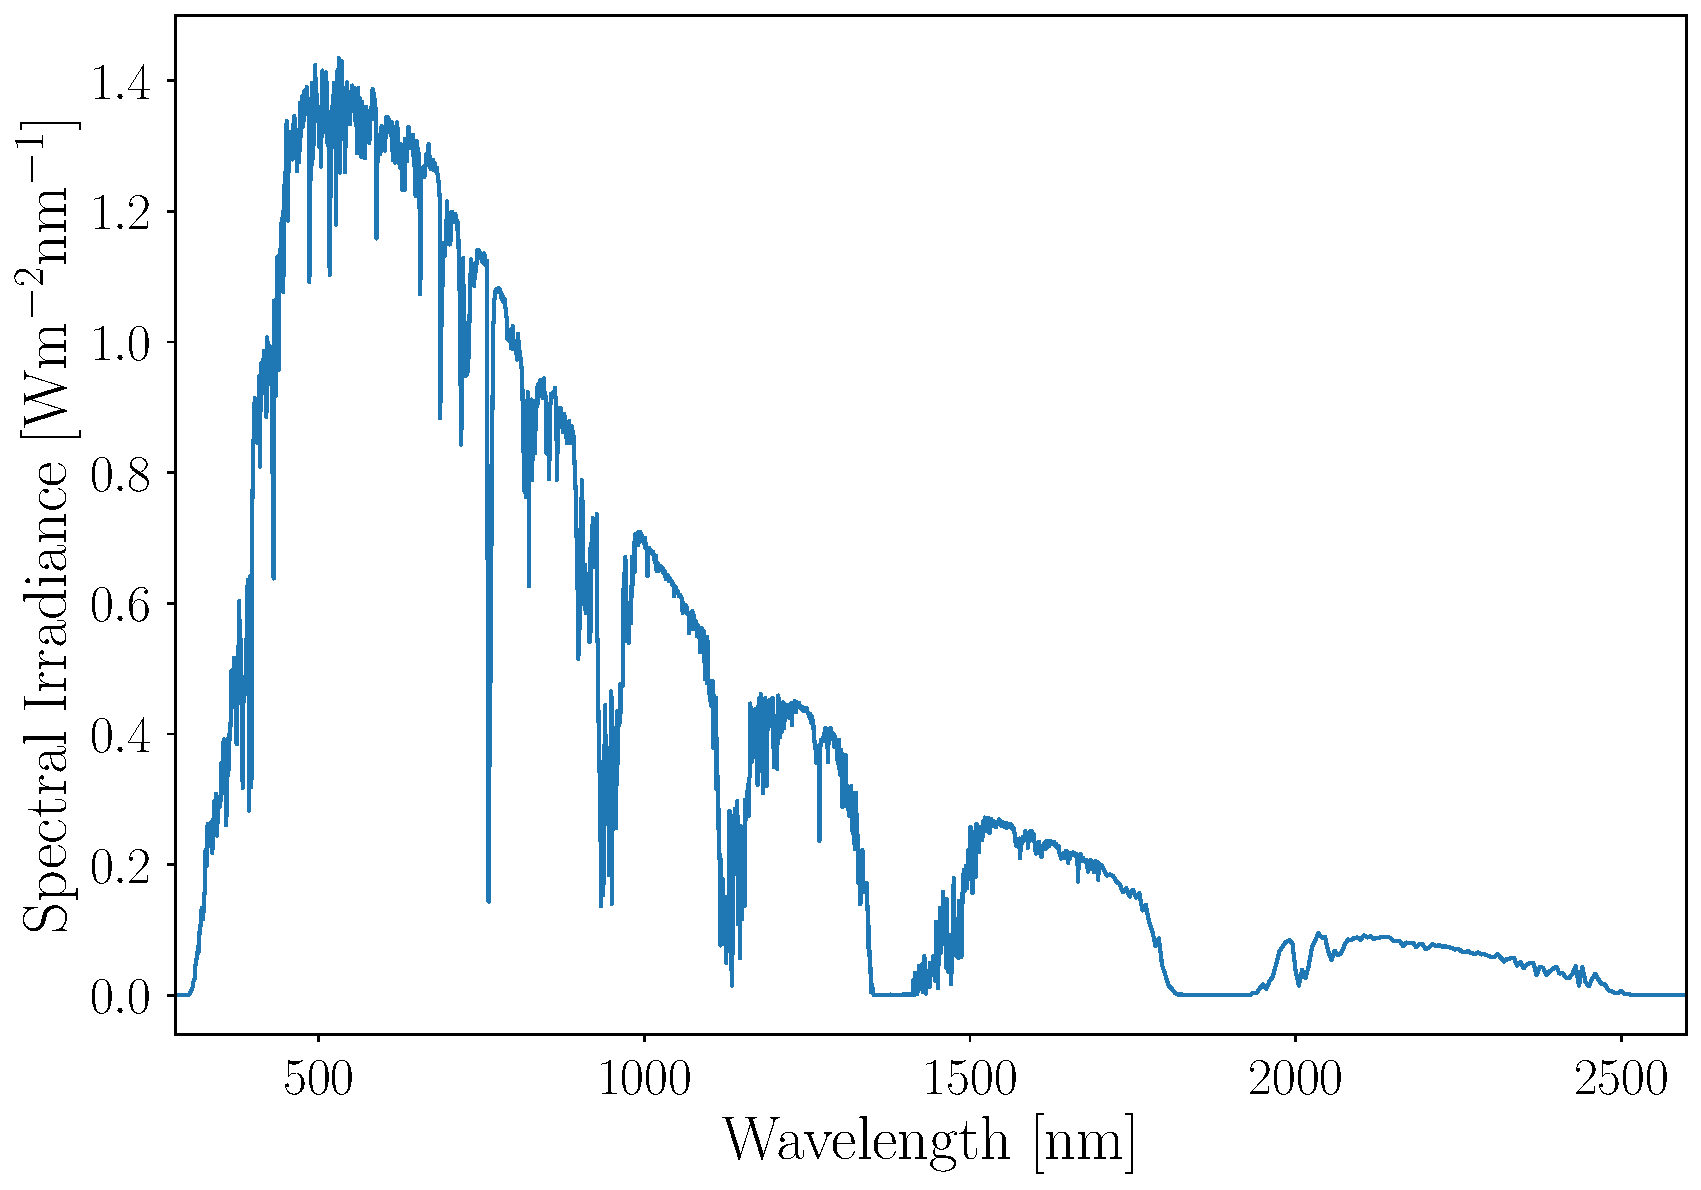
\includegraphics[width=\textwidth]{Spectral_Irradiance.pdf}
    \end{subfigure}
    \hfill
    \begin{subfigure}[b]{0.48\textwidth}
    	\centering
    	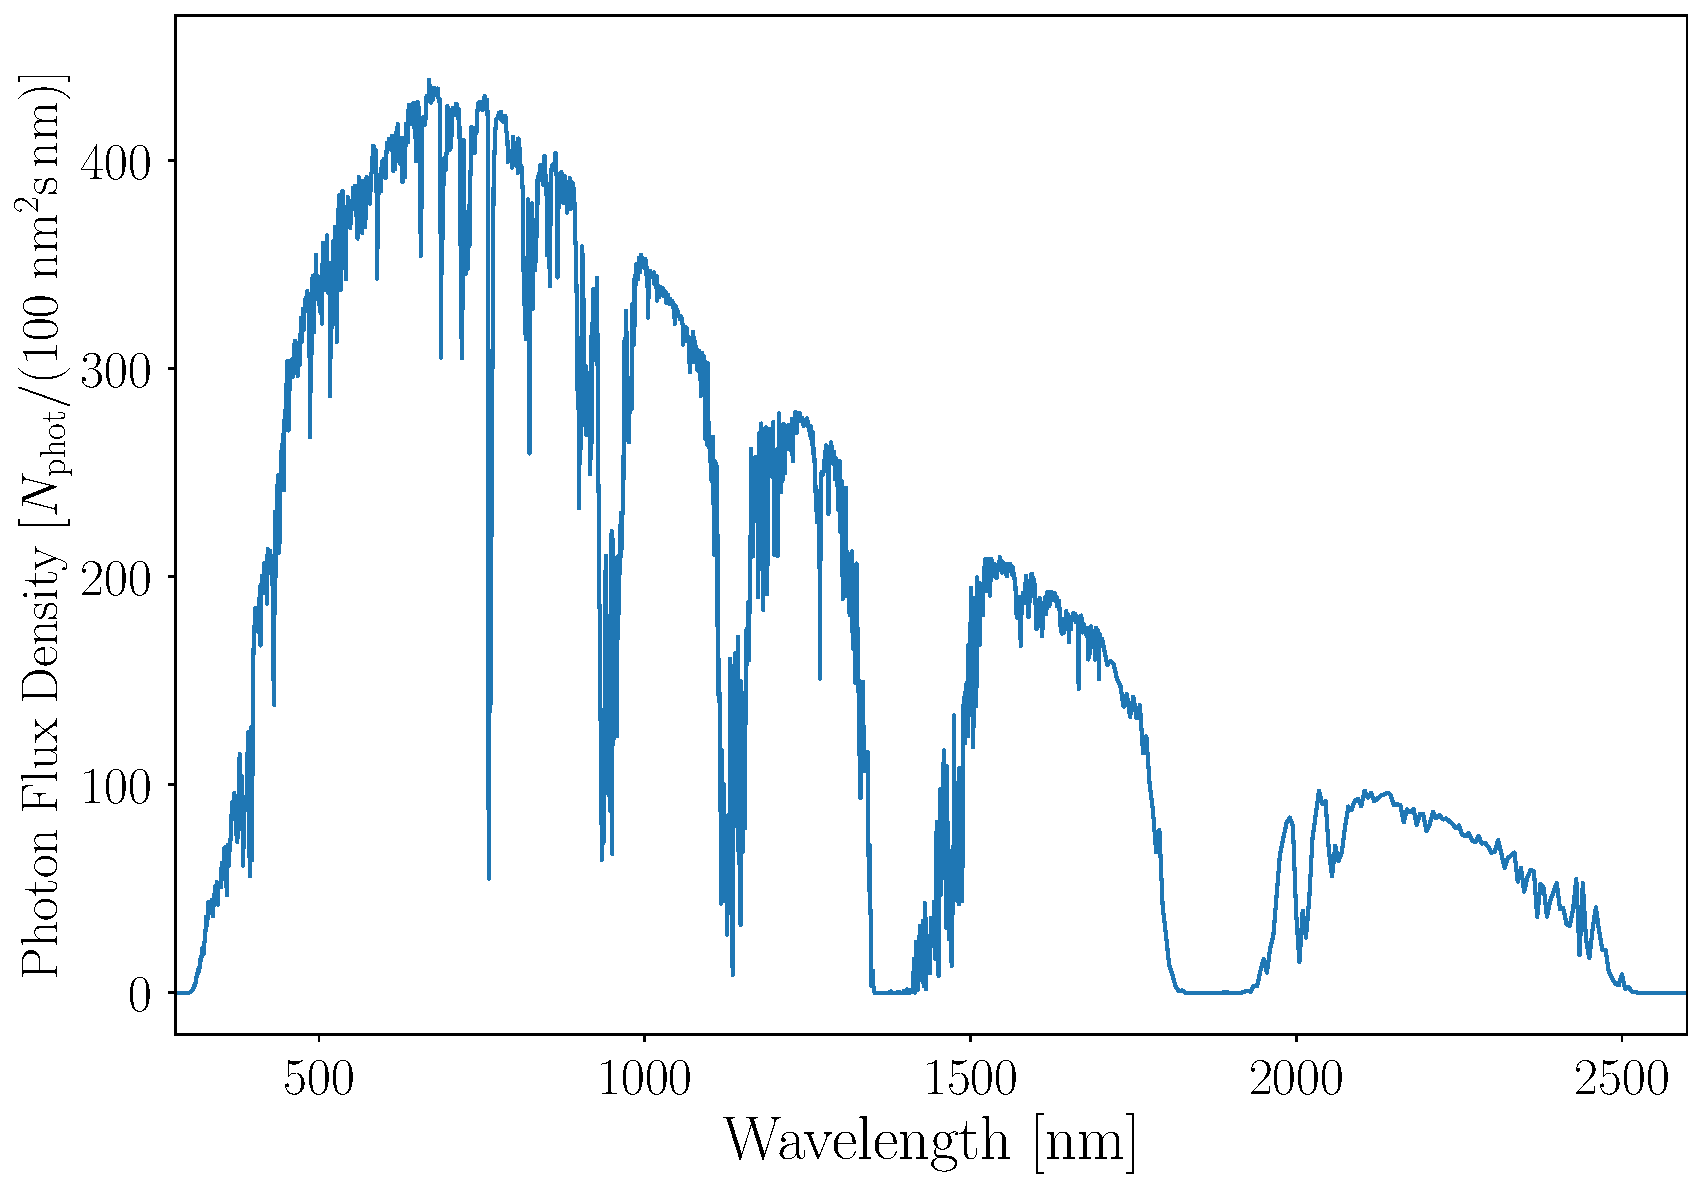
\includegraphics[width=\textwidth]{Photon_Flux_Density.pdf}
    \end{subfigure}
    \vskip\baselineskip
    \begin{subfigure}[b]{0.49\textwidth}  
    	\centering 
    	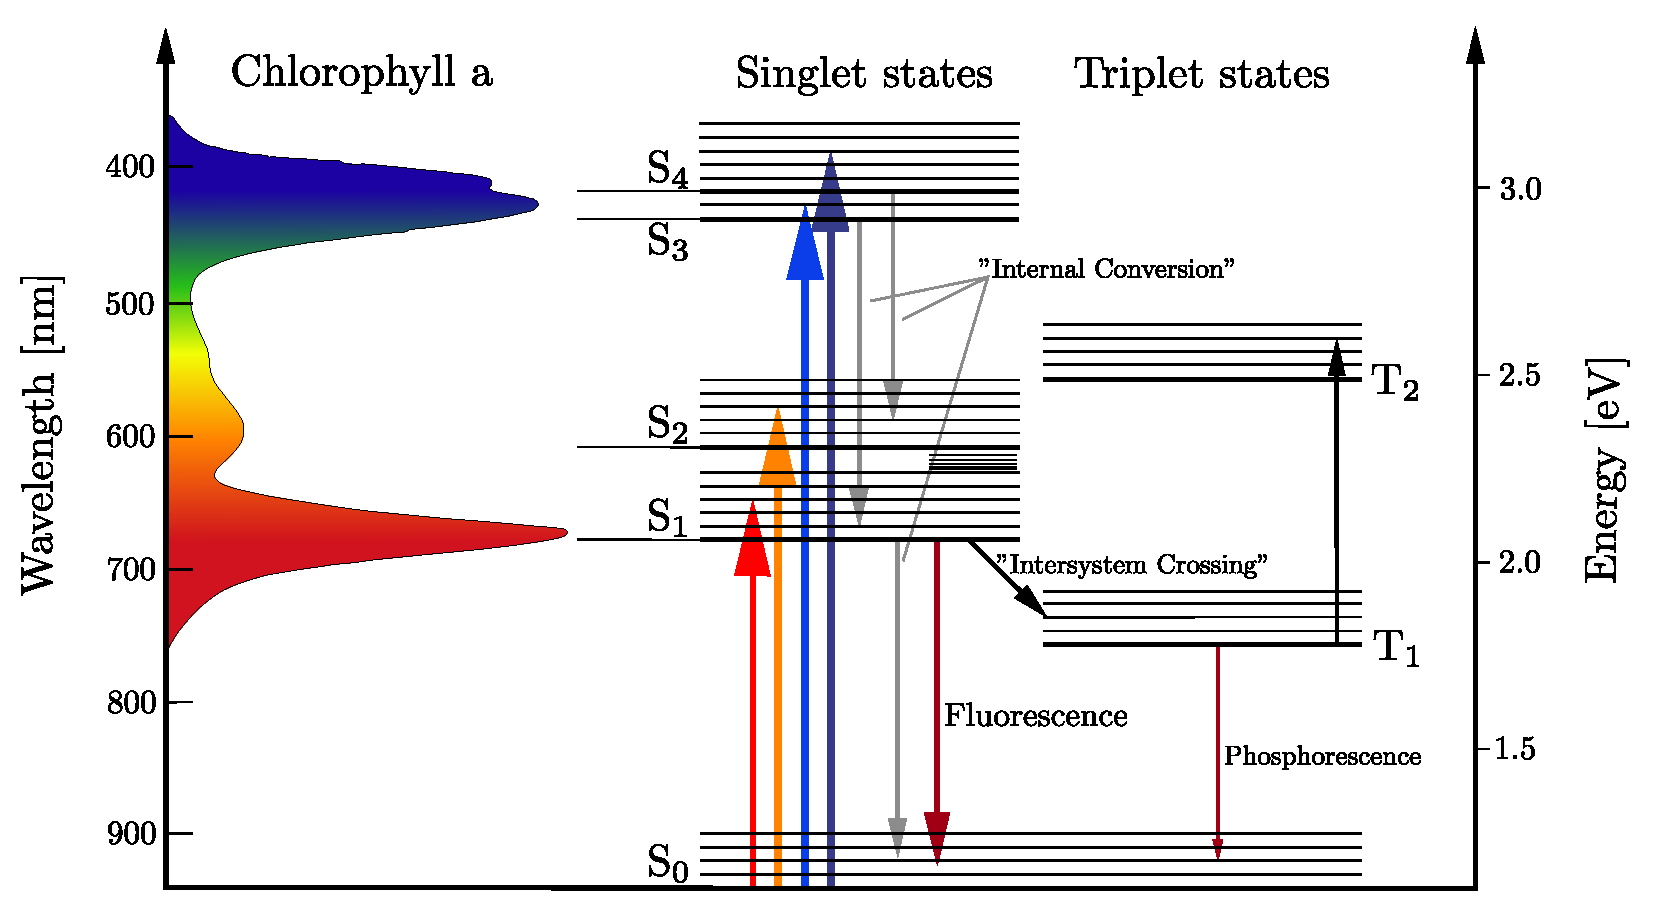
\includegraphics[width=\textwidth]{Jablonski_Diagramm.pdf}
    	\caption{Jablonski Diagram of a Chlorophyll a Molecule.}
    \end{subfigure}
    \hfill
    \begin{subfigure}[b]{0.49\textwidth}
    	\centering
    	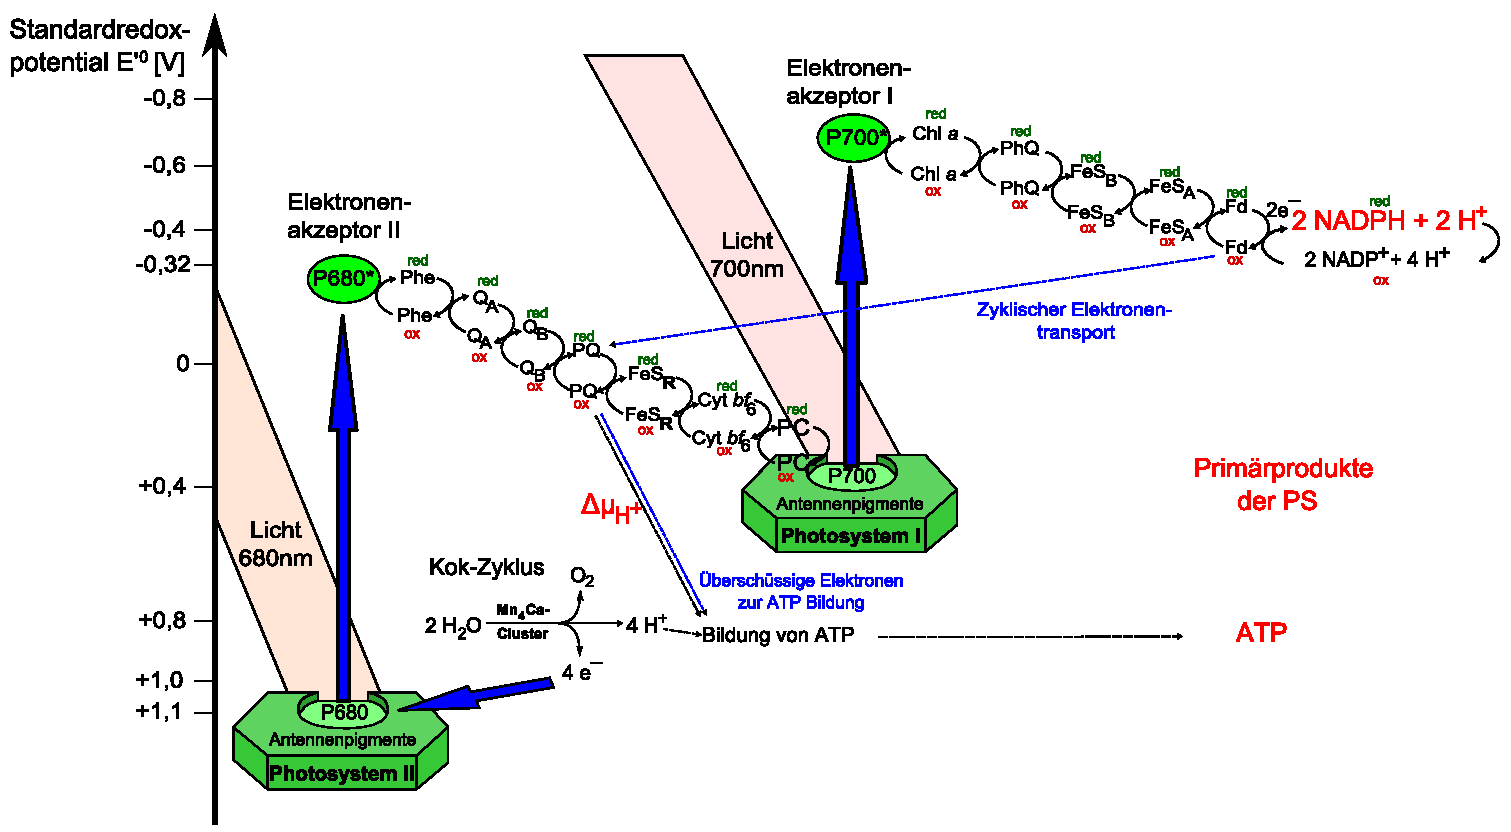
\includegraphics[width=\textwidth]{Z-Schema.pdf}
    	\caption{Z-Scheme of Photosynthesis.}
    \end{subfigure}
\end{figure}




\section{Photosynthetic Photon Flux Density (PPFD)}




\section{Simulation of EET}

In general, biochemical and biophysical processes can be described classically if the condition
\begin{equation}
\hbar\omega \ll k_{\mathrm{B}}T
\end{equation}
is fulfilled. This means that the thermal energy of a system $k_{\mathrm{B}}T$ overwhelmes the signatures of energy quantization so that discrete quantum jumps are so small that they appear as continuous processes when viewed on a larger scale.

\subsection{Born-Oppenheimer Separation}
Given the time-dependent Schrödinger equation
\begin{equation}
\mathrm{i}\hbar\frac{\partial}{\partial t}|\Psi(t)\rangle = \hat{H}|\Psi(t)\rangle
\end{equation}
with the general nonrelativistic molecular Hamiltonian
\begin{equation}
\hat{H} = -\sum_{\alpha=1}^{K}\frac{\hbar^2}{2m_{\alpha}}\nabla_{\boldsymbol{R}_{\alpha}}^{2} -\frac{\hbar^2}{2m_e}\sum_{i=1}^{N}\nabla_{\boldsymbol{r}_{i}}^{2}+\frac{1}{4\pi\varepsilon_0}\sum_{\alpha<\beta}^{K}\frac{Z_{\alpha}Z_{\beta}e^2}{\Vert\boldsymbol{R}_{\alpha}-\boldsymbol{R}_{\beta}\Vert}+\frac{1}{4\pi\varepsilon_0}\sum_{i<j}^{N}\frac{e^2}{\Vert\boldsymbol{r}_{i}-\boldsymbol{r}_{j}\Vert}-\frac{1}{4\pi\varepsilon_0}\sum_{\alpha=1}^{K}\sum_{i=1}^{N}\frac{Z_{\alpha}e^2}{\Vert\boldsymbol{r}_{i}-\boldsymbol{R}_{\alpha}\Vert}
\end{equation}
\begin{equation}
\Psi(\boldsymbol{r},\boldsymbol{R},t)=\sum_{a}\chi_{a}(\boldsymbol{R},t)\psi_{a}(\boldsymbol{r},\boldsymbol{R})
\end{equation}
\begin{align}
\hat{H}\Psi(\boldsymbol{r},\boldsymbol{R},t) &= (\hat{H}_{\mathrm{el}}+\hat{T}_{K})\sum_{a}\chi_{a}(\boldsymbol{R},t)\psi_{a}(\boldsymbol{r},\boldsymbol{R})\\
&= \sum_{a}E_{a}(\boldsymbol{R})\chi_{a}(\boldsymbol{R},t)\psi_{a}(\boldsymbol{r},\boldsymbol{R})+\sum_{a}\hat{T}_{K}\chi_{a}(\boldsymbol{R},t)\psi_{a}(\boldsymbol{r},\boldsymbol{R})\\
&=\mathrm{i}\hbar\frac{\partial}{\partial t}\sum_{a}\chi_{a}(\boldsymbol{R},t)\psi_{a}(\boldsymbol{r},\boldsymbol{R})
\end{align}
Multiplying with $\psi_{b}^{*}(\boldsymbol{r},\boldsymbol{R})$ from the left and integration over all electronic coordinates:
\begin{align}
\int\psi_{b}^{*}(\boldsymbol{r},\boldsymbol{R})\hat{H}\Psi_{a}(\boldsymbol{r},\boldsymbol{R},t)\mathrm{d}\boldsymbol{r} &= E_{b}(\boldsymbol{R})\chi_{b}(\boldsymbol{R},t)\\
&\quad+\sum_{a}\int\psi_{b}^{*}(\boldsymbol{r},\boldsymbol{R})\hat{T}_{K}\chi_{a}(\boldsymbol{R},t)\psi_{a}(\boldsymbol{r},\boldsymbol{R})\mathrm{d}\boldsymbol{r}\label{nonadiabaticity}\\
&=\mathrm{i}\hbar\frac{\partial}{\partial t}\chi_{b}(\boldsymbol{R},t)
\end{align}
\begin{align}
\hat{T}_{K}\chi_{a}(\boldsymbol{R},t)\psi_{a}(\boldsymbol{r},\boldsymbol{R}) &= -\sum_{\alpha=1}^{K}\frac{\hbar^2}{2m_{\alpha}}\nabla_{\boldsymbol{R}_{\alpha}}\chi_{a}(\boldsymbol{R},t)\psi_{a}(\boldsymbol{r},\boldsymbol{R})\\
&= -\sum_{\alpha=1}^{K}\frac{\hbar^2}{2m_{\alpha}}\Big(\nabla_{\boldsymbol{R}_{\alpha}}\big(\chi_{a}(\boldsymbol{R},t)\nabla_{\boldsymbol{R}_{\alpha}}\psi_{a}(\boldsymbol{r},\boldsymbol{R})+\psi_{a}(\boldsymbol{r},\boldsymbol{R})\nabla_{\boldsymbol{R}_{\alpha}}\chi_{a}(\boldsymbol{R},t)\big)\Big)\\
&=-\sum_{\alpha=1}^{K}\frac{\hbar^2}{2m_{\alpha}}\Big(\chi_{a}(\boldsymbol{R},t)\nabla_{\boldsymbol{R}_{\alpha}}^{2}\psi_{a}(\boldsymbol{r},\boldsymbol{R})\\
&\quad+2\nabla_{\boldsymbol{R}_{\alpha}}\chi_{\alpha}(\boldsymbol{R},t)\nabla_{\boldsymbol{R}_{\alpha}}\psi_{a}(\boldsymbol{r},\boldsymbol{R})+\psi_{a}(\boldsymbol{r},\boldsymbol{R})\nabla_{\boldsymbol{R}_{\alpha}}^{2}\chi_{a}(\boldsymbol{R},t)\Big)
\end{align}
The expression \eqref{nonadiabaticity} can now be written as
\begin{align}
\sum_{a}\Big(-\sum_{\alpha=1}^{K}\frac{\hbar^2}{2m_{\alpha}}\int\psi_{b}^{*}(\boldsymbol{r},\boldsymbol{R})\nabla_{\boldsymbol{R}_{\alpha}}^{2}&\psi_{a}(\boldsymbol{r},\boldsymbol{R})\mathrm{d}\boldsymbol{r}\chi_{a}(\boldsymbol{R},t)-\sum_{\alpha=1}^{K}\frac{\hbar^2}{m_{\alpha}}\int\psi_{b}^{*}(\boldsymbol{r},\boldsymbol{R})\nabla_{\boldsymbol{R}_{\alpha}}\psi_{a}(\boldsymbol{r},\boldsymbol{R})\mathrm{d}\boldsymbol{r}\nabla_{\boldsymbol{R}_{\alpha}}\chi_{a}(\boldsymbol{R},t)\Big)\\
&-\sum_{a}\underbrace{\int\psi_{b}^{*}(\boldsymbol{r},\boldsymbol{R})\psi_{a}(\boldsymbol{r},\boldsymbol{R})\mathrm{d}\boldsymbol{r}}_{=\delta_{a,b}}\sum_{\alpha=1}^{K}\frac{\hbar^2}{2m_{\alpha}}\nabla_{\boldsymbol{R}_{\alpha}}^{2}\chi_{a}(\boldsymbol{R},t)
\end{align}
\begin{align}
\hat{\Theta}_{ba} &= \int\Psi_{b}^{*}(\boldsymbol{r},\boldsymbol{R})\hat{T}_{K}\psi_{a}(\boldsymbol{r},\boldsymbol{R})\mathrm{d}\boldsymbol{r}-\sum_{\alpha=1}^{K}\frac{\hbar^2}{m_{\alpha}}\int\psi_{b}^{*}(\boldsymbol{r},\boldsymbol{R})\nabla_{\boldsymbol{R}_{\alpha}}\psi_{a}(\boldsymbol{r},\boldsymbol{R})\mathrm{d}\boldsymbol{r}\nabla_{\boldsymbol{R}_{\alpha}}\\
&=\big\langle\psi_{b}\big|\hat{T}_{K}\big|\psi_{a}\big\rangle -\sum_{\alpha=1}^{K}\frac{\hbar^2}{m_{\alpha}}\big\langle\psi_{b}\big|\nabla_{\boldsymbol{R}_{\alpha}}\big|\psi_{a}\big\rangle\nabla_{\boldsymbol{R}_{\alpha}}
\end{align}
\begin{equation}
\big(E_{b}(\boldsymbol{R})+\hat{T}_{K}\big)\chi_{b}(\boldsymbol{R},t)+\sum_{a}\hat{\Theta}_{ba}\chi_{a}(\boldsymbol{R},t) = \mathrm{i}\hbar\frac{\partial}{\partial t}\chi_{b}(\boldsymbol{R},t)
\end{equation}
It is possible to split up the time-dependent vibrational wavefunctions into two independent functions which depend on only the nuclear coordinates and only on the time coordinate:
\begin{equation}
h
\end{equation}
\begin{equation}
\big(E_{b}(\boldsymbol{R})+\hat{T}_{K}\big)\chi_{b}^{\nu}(\boldsymbol{R})+\sum_{a}\hat{\Theta}_{ba}\chi_{a}^{\nu}(\boldsymbol{R})=E_{\nu}\chi_{b}^{\nu}(\boldsymbol{R})
\end{equation}
\begin{align}
\renewcommand{\arraystretch}{1.2}
\left(\begin{array}{cccc}
E_{1}(\boldsymbol{R}) & 0  &  \cdots  &  0
\\
0 & E_{2}(\boldsymbol{R})  &  \cdots  &  0
\\
\vdots  &  \vdots  &  \ddots  &  \vdots
\\
0  &  0  &  \cdots  &  E_{b}(\boldsymbol{R})
\\
\end{array}\right)
\left(\begin{array}{c}
\chi_{1}^{\nu}(\boldsymbol{R})
\\
\chi_{2}^{\nu}(\boldsymbol{R})
\\
\vdots
\\
\chi_{b}^{\nu}(\boldsymbol{R})
\\
\end{array}\right)
+
\left(\begin{array}{cccc}
\hat{T}_{K} & 0  &  \cdots  &  0
\\
0 & \hat{T}_{K}  &  \cdots  &  0
\\
\vdots  &  \vdots  &  \ddots  &  \vdots
\\
0  &  0  &  \cdots  &  \hat{T}_{K}
\\
\end{array}\right)
\left(\begin{array}{c}
\chi_{1}^{\nu}(\boldsymbol{R})
\\
\chi_{2}^{\nu}(\boldsymbol{R})
\\
\vdots
\\
\chi_{b}^{\nu}(\boldsymbol{R})
\\
\end{array}\right)
\\
+
\renewcommand{\arraystretch}{1.2}
\left(\begin{array}{cccc}
\hat{\Theta}_{11} & \hat{\Theta}_{12}  &  \cdots  &  \hat{\Theta}_{1a}
\\
\hat{\Theta}_{21} & \hat{\Theta}_{22}  &  \cdots  &  \hat{\Theta}_{2a}
\\
\vdots  &  \vdots  &  \ddots  &  \vdots
\\
\hat{\Theta}_{b1}  &  \hat{\Theta}_{b2}  &  \cdots  &  \hat{\Theta}_{ba}
\\
\end{array}\right)
\left(\begin{array}{c}
\chi_{1}^{\nu}(\boldsymbol{R})
\\
\chi_{2}^{\nu}(\boldsymbol{R})
\\
\vdots
\\
\chi_{b}^{\nu}(\boldsymbol{R})
\\
\end{array}\right)
= E_{\nu}
\left(\begin{array}{c}
\chi_{1}^{\nu}(\boldsymbol{R})
\\
\chi_{2}^{\nu}(\boldsymbol{R})
\\
\vdots
\\
\chi_{b}^{\nu}(\boldsymbol{R})
\\
\end{array}\right)\qquad\qquad\qquad
\end{align}
\begin{equation}
\hat{H}|\Psi_{\nu}\rangle = E_{\nu}|\Psi_{\nu}\rangle
\end{equation}
\begin{equation}
\Psi_{\nu}(\boldsymbol{r},\boldsymbol{R}) = \sum_{a}\chi_{a}^{\nu}(\boldsymbol{R})\psi_{a}(\boldsymbol{r},\boldsymbol{R})
\end{equation}






\subsubsection{Born-Huang Approximation}
\subsubsection{Born-Oppenheimer Approximation}








\subsection{Frenkel Exciton Hamiltonian}
The Fenna-Matthews-Olsen complex (FMO) is a chromophore-protein complex in green sulfur bacteria which has been extensively used as a model complex for larger antenna complexes in the last 30 years. In these photosynthetic antenna complexes, high energy photons from sunlight are absorbed by specific bacteriochlorophylls. These bacteriochlorophylls are embedded in a protein skeleton which is responsible for the correct orientation of the chromophores with respect to each other and for the finetuning of the energy levels. There are different interactions between the chromophores and their environment that are assumed to influence the optical transition energies of the chromophores:
\begin{itemize}
	\item Different solvent environments which cause differences for example in Mg$^{2+}$ ligation and chlorophyll side chain polarisation
	\item Differences in H-bonding
	\item Electrostatic interactions with charged and aromatic amino-acid side chains of the protein
	\item Differences in the conformation of the chromophore; for example, the degree of planarity and the rotation angle of the acetyl group
	\item Direct electrostatic coupling between chromophores; at very short distances even exchange interaction comes into play
\end{itemize}
The goal is now to derive the Hamiltonian for a multichromophoric system such as the Fenna-Matthews-Olsen complex (FMO). The first step is to extract all bacteriochlorophylls and their geometries from the FMO complex and construct a Hamiltonian for this isolated system. This can be done by taking the sum of the individual chromophore Hamiltonians and adding the potential energy terms for the interaction between all chromophores:
\begin{align}
\hat{H}_{\mathrm{FMO}}&=\sum_{m}\hat{H}_{m}+\frac{1}{2}\sum_{m,n}\hat{V}_{mn}\\
&= \sum_{m}\big(\hat{T}_m+\hat{H}_m^{\mathrm{(e)}}\big)+\frac{1}{2}\sum_{m,n}\big(\hat{V}_{mn}^{\mathrm{(e-e)}}+\hat{V}_{mn}^{\mathrm{(n-n)}}+\hat{V}_{mn}^{(e-n)}\big)
\end{align}
It can be clearly seen that this operator intrinsically contains the fourth and the fifth contribution to the energy shifts mentioned above. In order to go into a suitable matrix representation of this Hamiltonian, we choose the eigenstates of the electronic Hamiltonian $\hat{H}_{m}^{\mathrm{(e)}}$ for isolated single chromophores as building blocks:
\begin{equation}
\hat{H}_{m}^{\mathrm{(e)}}|\psi_{ma}\rangle = U_{ma}|\psi_{ma}\rangle
\end{equation}
Here the energy eigenvalues $U_{ma}$ for a specific set of nuclear coordinates $\{\vec{R}_j\}$ are essentially the energies of the adiabatic states denoted by $a\in \{S_0, S_1, T_1,...\}$. Theoretically they are equivalent to the Full Configuration Interaction (FCI) solutions. Now the basis functions for the Hamiltonian $\hat{H}_{\mathrm{FMO}}$ can be expressed as a Hartree product of single chromophore eigenstates:
\begin{equation}
|\Psi_A\rangle = \prod_{m=1}^{N}|\psi_{ma}\rangle
\end{equation}
The assumption of a symmetric Hartree product instead of an antisymmetric Slater determinant is only valid if the chromophores are clearly separated from each other since the exchange interaction begins to significantly contribute to the energy at very short distances. The expansion of the Hamiltonian in terms of these product states leads to the following matrix representation:
\begin{align}
H_{\mathrm{FMO}} &= \sum_{A}|\Psi_{A}\rangle\langle\Psi_{A}|\hat{H}_{\mathrm{FMO}}\sum_{B}|\Psi_{B}\rangle\langle\Psi_{B}|\\
&= \sum_{A,B}\langle\Psi_{A}|\hat{H}_{\mathrm{FMO}}|\Psi_{B}\rangle|\Psi_{A}\rangle\langle\Psi_{B}|\\
&= \sum_{A,B}\Big(\sum_{m}\langle\Psi_{A}|\hat{H}_{m}|\Psi_{B}\rangle +\frac{1}{2}\sum_{m,n}\langle\Psi_{A}|\hat{V}_{mn}|\Psi_{B}\rangle\Big)|\Psi_{A}\rangle\langle\Psi_{B}|\\
&= \sum_{a,b}\Big(\sum_{m}\prod_{k}\langle\psi_{ka}|\hat{H}_{m}|\psi_{kb}\rangle +\frac{1}{2}\sum_{m,n}\prod_{k}\langle\psi_{ka}|\hat{V}_{mn}|\psi_{kb}\rangle\Big)\prod_{k}|\psi_{ka}\rangle\prod_{k}\langle\psi_{kb}|\\
&= \sum_{a,b}\sum_{m}\langle\psi_{ma}|\hat{H}_{m}|\psi_{mb}\rangle\prod_{k\neq m}\langle\psi_{ka}|\psi_{ka}\rangle\langle\psi_{kb}|\psi_{kb}\rangle|\psi_{ma}\rangle\langle\psi_{mb}|\\
&\quad + \frac{1}{2}\sum_{a,b}\sum_{m,n}\langle\psi_{ma}\psi_{na}|\hat{V}_{mn}|\psi_{mb}\psi_{nb}\rangle\prod_{k\neq m,n}\langle\psi_{ka}|\psi_{ka}\rangle\langle\psi_{kb}|\psi_{kb}\rangle|\psi_{ma}\rangle\langle\psi_{mb}|\\
&= \sum_{a,b}\sum_{m}\langle\psi_{ma}|\hat{H}_{m}|\psi_{mb}\rangle|\psi_{ma}\rangle\langle\psi_{mb}| + \frac{1}{2}\sum_{a,b}\sum_{m,n}\langle\psi_{ma}\psi_{na}|\hat{V}_{mn}|\psi_{mb}\psi_{nb}\rangle|\psi_{ma}\rangle\langle\psi_{mb}|
\end{align}





\subsubsection{Direct Coupling between Chromophores}
Förster dipole-dipole coupling:

\subsubsection{Electrochromic Shifts}




\subsection{Molecular Vibrations}
\url{https://chemistry.stackexchange.com/questions/67460/do-different-vibrational-modes-correspond-to-vibrational-energy-levels}\\
\url{https://aip.scitation.org/doi/10.1063/1.2710256}\\
\url{https://manual.q-chem.com/5.2/Ch11.S11.SS1.html}

\subsubsection{Harmonic Approximation}
\subsubsection{Vibrational Configuration Interaction (VCI)}


\subsection{Boltzmann Distribution}



\subsection{Exciton-Phonon Coupling}


\subsection{Exciton-Photon Coupling}

Usually the coupling of a molecular system to the electromagnetic field is accounted for by using the minimal coupling Hamiltonian. The total molecular Hamiltonian coupled to the electromagnetic field can be written as
\begin{equation}
\hat{H}_{\mathrm{mol}} = -\sum_{i=1}^{N}\frac{1}{2m_{e}}\big(\hat{\boldsymbol{p}}_{i}-e\hat{\boldsymbol{A}}(\boldsymbol{r}_{i})\big)^{2} - \sum_{j=1}^{K}\frac{1}{2m_{j}}\big(\hat{\boldsymbol{p}}_{j}-Z_{j}e\hat{\boldsymbol{A}}(\boldsymbol{r}_{j})\big)^{2} +\hat{V}_{KK}+\hat{V}_{ee}+\hat{V}_{Ke}
\end{equation}
The minimal coupling part of the total Hamiltonian can be simplified further:
\begin{align}
\hat{H}_{\mathrm{min}} &= -\sum_{i=1}^{N}\frac{1}{2m_{e}}\big(\hat{\boldsymbol{p}}_{i}-e\hat{\boldsymbol{A}}(\boldsymbol{r}_{i})\big)^{2} - \sum_{j=1}^{K}\frac{1}{2m_{j}}\big(\hat{\boldsymbol{p}}_{j}-Z_{j}e\hat{\boldsymbol{A}}(\boldsymbol{r}_{j})\big)^{2}\\
&= -\sum_{i=1}^{N}\Big(\frac{1}{2m_e}\hat{\boldsymbol{p}}_{i}^{2}-\frac{e}{m_e}\hat{\boldsymbol{p}}_{i}\hat{\boldsymbol{A}}(\boldsymbol{r}_i)+\underbrace{\frac{e^2}{2m_e}\hat{\boldsymbol{A}}^2(\boldsymbol{r}_i)}_{\approx 0}\Big) -\sum_{j=1}^{K}\Big(\frac{1}{2m_{j}}\hat{\boldsymbol{p}}_{j}^{2}-\frac{eZ_{j}}{m_j}\hat{\boldsymbol{p}}_{j}\hat{\boldsymbol{A}}(\boldsymbol{r}_j)+\underbrace{\frac{e^{2}Z_{j}^2}{2m_j}\hat{\boldsymbol{A}}^2(\boldsymbol{r}_j)}_{\approx 0}\Big)\\
&= -\sum_{i=1}^{N}\frac{\hbar^2}{2m_e}\nabla_{i}^{2}-\sum_{j=1}^{K}\frac{\hbar^2}{2m_{j}}\nabla_{j}^{2}+\underbrace{\sum_{i=1}^{N}\frac{e}{m_e}\hat{\boldsymbol{p}}_{i}\hat{\boldsymbol{A}}(\boldsymbol{r}_{i})+\sum_{j=1}^{K}\frac{eZ_{j}}{m_{j}}\hat{\boldsymbol{p}}_{j}\hat{\boldsymbol{A}}(\boldsymbol{r}_{j})}_{=\hat{H}_{\mathrm{int}}}
\end{align}
The vector potential operator is given by
\begin{equation}
\hat{\boldsymbol{A}}(\boldsymbol{r}_i)=\sum_{k}\boldsymbol{e}_{k}\frac{1}{\omega_k}N_{k}\Big(\hat{a}_{k}\exp(\mathrm{i}\boldsymbol{k}_{k}\boldsymbol{r}_i)+\hat{a}_{k}^{\dagger}\exp(-\mathrm{i}\boldsymbol{k}_{k}\boldsymbol{r}_i)\Big)
\end{equation}
The exponentials can be expanded in a Taylor series. In the so called electric Dipole approximation these exponentials can be approximately set to 1:
\begin{align}
\exp(\mathrm{i}\boldsymbol{k}_{k}\boldsymbol{r}_{i})&=\sum_{n=0}^{\infty}\frac{(\mathrm{i}\boldsymbol{k}_{k}\boldsymbol{r}_i)^n}{n!}=1+\mathrm{i}\boldsymbol{k}_{k}\boldsymbol{r}_{i}-\frac{1}{2}(\boldsymbol{k}_{k}\boldsymbol{r}_i)^2+\cdots\approx 1\\
\exp(-\mathrm{i}\boldsymbol{k}_{k}\boldsymbol{r}_{i})&=\sum_{n=0}^{\infty}\frac{(-\mathrm{i}\boldsymbol{k}_{k}\boldsymbol{r}_i)^n}{n!}=1-\mathrm{i}\boldsymbol{k}_{k}\boldsymbol{r}_{i}+\frac{1}{2}(\boldsymbol{k}_{k}\boldsymbol{r}_i)^2-\cdots\approx 1
\end{align}
Plugging the vector potential operator in the dipole approximation into the interaction Hamiltonian, we arrive at
\begin{align}
\hat{H}_{\mathrm{int}} &= \sum_{i=1}^{N}\frac{e}{m_e}\sum_{k}\frac{1}{\omega_k}N_{k}\boldsymbol{e}_{k}\hat{\boldsymbol{p}}_{i}\big(\hat{a}_{k}+\hat{a}_{k}^{\dagger}\big) + \sum_{j=1}^{K}\frac{eZ_{j}}{m_{j}}\sum_{k}\frac{1}{\omega_k}N_{k}\boldsymbol{e}_{k}\hat{\boldsymbol{p}}_{j}\big(\hat{a}_{k}+\hat{a}_{k}^{\dagger}\big)\\
&= \bigg(\sum_{i=1}^{N}\frac{e}{m_e}\hat{\boldsymbol{p}}_{i}+\sum_{j=1}^{K}\frac{eZ_{j}}{m_{j}}\hat{\boldsymbol{p}}_{j}\bigg)\sum_{k}\frac{1}{\omega_k}N_{k}\boldsymbol{e}_{k}\big(\hat{a}_{k}+\hat{a}_{k}^{\dagger}\big)
\end{align}
To find a simpler expression for the momentum operators, they will be expanded in terms of eigenstates of the unperturbed total molecular Hamiltonian and replaced by position operators, using the quantum version of Newton's first law:
\begin{align}
\langle\Psi_{a}(t)|\hat{\boldsymbol{p}}_{i}|\Psi_{b}(t)\rangle &= -\mathrm{i}\hbar m_e\frac{\mathrm{d}}{\mathrm{d}t}\langle\Psi_{a}(t)|\hat{\boldsymbol{r}}_{i}|\Psi_{b}(t)\rangle = -\mathrm{i}\hbar m_e\frac{\mathrm{d}}{\mathrm{d}t}\int e^{\mathrm{i}E_{a}t/\hbar}\Psi_{a}^{*}(\{\boldsymbol{r}\})\boldsymbol{r}_{i}e^{-\mathrm{i}E_{b}t/\hbar}\Psi_{b}(\{\boldsymbol{r}\})\mathrm{d}\boldsymbol{r}\\
&= \hbar m_{e}\frac{E_{a}-E_{b}}{\hbar}\langle\Psi_{a}(t)|\hat{\boldsymbol{r}}_{i}|\Psi_{b}(t)\rangle = \hbar m_{e}\omega_{k}\langle\Psi_{a}(t)|\hat{\boldsymbol{r}}_{i}|\Psi_{b}(t)\rangle
\end{align}
For the nuclear momentum operator the result is analogous:
\begin{equation}
\langle\Psi_{a}(t)|\hat{\boldsymbol{p}}_{j}|\Psi_{b}(t)\rangle = \hbar m_{j}\omega_{k}\langle\Psi_{a}(t)|\hat{\boldsymbol{r}}_{j}|\Psi_{b}(t)\rangle
\end{equation}
Inserting these expressions into the interaction Hamiltonian and suppressing the time-dependent part of the wavefunction leads to the final expression
\begin{equation}
\hat{H}_{\mathrm{int}} = \hbar\langle\Psi_{a}|\hat{\boldsymbol{\mu}}|\Psi_{b}\rangle\sum_{k}N_{k}\boldsymbol{e}_{k}\big(\hat{a}_{k}+\hat{a}_{k}^{\dagger}\big)
\end{equation}
with the transition dipole moment operator
\begin{equation}
\hat{\boldsymbol{\mu}} = \sum_{i=1}^{N}e\boldsymbol{r}_{i}+\sum_{j=1}^{K}eZ_{j}\boldsymbol{r}_{j} = \hat{\boldsymbol{\mu}}_{\mathrm{el}}+\hat{\boldsymbol{\mu}}_{\mathrm{nuc}}
\end{equation}
The corresponding operator matrix in the eigenbasis of the unperturbed Hamiltonian can be written as
\begin{equation}
\renewcommand{\arraystretch}{1.3}
\boldsymbol{\mu}
=
\left(\begin{array}{cccc}
\langle\Psi_{1}|\hat{\boldsymbol{\mu}}|\Psi_{1}\rangle & \langle\Psi_{1}|\hat{\boldsymbol{\mu}}|\Psi_{2}\rangle  &  \cdots  &  \langle\Psi_{1}|\hat{\boldsymbol{\mu}}|\Psi_{b}\rangle
\\
\langle\Psi_{2}|\hat{\boldsymbol{\mu}}|\Psi_{1}\rangle & \langle\Psi_{2}|\hat{\boldsymbol{\mu}}|\Psi_{2}\rangle  &  \cdots  &  \langle\Psi_{2}|\hat{\boldsymbol{\mu}}|\Psi_{b}\rangle
\\
\vdots  &  \vdots  &  \ddots  &  \vdots
\\
\langle\Psi_{a}|\hat{\boldsymbol{\mu}}|\Psi_{1}\rangle  &  \langle\Psi_{a}|\hat{\boldsymbol{\mu}}|\Psi_{2}\rangle  &  \cdots  &  \langle\Psi_{a}|\hat{\boldsymbol{\mu}}|\Psi_{b}\rangle
\\
\end{array}\right)
\end{equation}

\subsubsection{Franck-Condon Principle}












\subsection{Total Hamiltonian}
\begin{equation}
\hat{H} = \underbrace{\sum_{m=1}^{N}\varepsilon_{m}\hat{a}_{m}^{\dagger}\hat{a}_{m}+\sum_{n<m}J_{mn}(\hat{a}_{m}^{\dagger}\hat{a}_{n}+\hat{a}_{n}^{\dagger}\hat{a}_{m})}_{\hat{H}_{\mathrm{ex}}} + \underbrace{\sum_{i}\hbar\omega_{i}\hat{a}_{i}^{\dagger}\hat{a}_{i}+\sum_{k}\hbar\omega_{k}\hat{a}_{k}^{\dagger}\hat{a}_{k}}_{\hat{H}_{\mathrm{phot}}+\hat{H}_{\mathrm{phon}}}+\hat{\boldsymbol{\mu}}\sum_{k}N_{k}\boldsymbol{e}_{k}\big(\hat{a}_{k}+\hat{a}_{k}^{\dagger}\big)
\end{equation}


\subsection{Liouville-von Neumann Equation}
In the following section open quantum systems will be discussed in detail. The basic assumption of this theory is that you can split the Hamiltonian of an open quantum system into three parts:
\begin{equation}
\hat{H}=\hat{H}_{\mathrm{S}}+\hat{H}_{\mathrm{R}}+\hat{H}_{\mathrm{SR}}
\end{equation}
Here $\hat{H}_{\mathrm{S}}$ is the Hamiltonian of the system we are interested in, $\hat{H}_{\mathrm{R}}$ is the reservoir Hamiltonian and $\hat{H}_{\mathrm{SR}}$ is the Hamiltonian of the system-reservoir coupling. The whole systems time evolution is governed by the time dependent Schrödinger equation:
\begin{equation}
\mathrm{i}\hbar\frac{\partial}{\partial t}|\Psi_{\nu}(t)\rangle = \hat{H}|\Psi_{\nu}(t)\rangle
\end{equation}
With the help of a Taylor series expansion with respect to time one can find a formal solution of the time dependent Schrödinger equation:
\begin{equation}
|\Psi_{\nu}(t)\rangle = e^{-\mathrm{i}\hat{H}t/\hbar}|\Psi_{\nu}(t_0)\rangle = \hat{U}(t) |\Psi_{\nu}(t_0)\rangle
\end{equation}
In the real world a system never is in a single state all the time. A real system is in a classical mixture of eigenstates described by a density operator:
\begin{equation}
\hat{\rho}(t) = \sum_{\nu}P_{\nu}|\Psi_{\nu}(t)\rangle\langle\Psi_{\nu}(t)|\label{Density Operator}
\end{equation}
The classical, time independent probability of the system being in the $\nu$-th state is described by $P_{\nu}$. If we apply the unitary time evolution operator $\hat{U}(t)$ onto the density operator, it transforms into the following form:
\begin{equation}
\hat{\rho}(t) = \sum_{\nu}P_{\nu}\hat{U}(t)|\Psi_{\nu}(t_0)\rangle\langle\Psi_{\nu}(t_0)|\hat{U}^{\dagger}(t) = \hat{U}(t)\hat{\rho}(t_0)\hat{U}^{\dagger}(t)
\end{equation}
In order to derive an equation of motion (EOM) for the density operator, its derivative with respect to time is calculated:
\begin{align}
\frac{\partial}{\partial t}\hat{\rho}(t) &= \sum_{\nu}P_{\nu}\Big(\frac{\partial}{\partial t}|\Psi_{\nu}(t)\rangle\Big)\langle\Psi_{\nu}(t)|+\sum_{\nu}P_{\nu}|\Psi_{\nu}(t)\rangle\Big(\frac{\partial}{\partial t}\langle\Psi_{\nu}(t)|\Big)\\
&= \sum_{\nu}P_{\nu}\Big(-\frac{\mathrm{i}}{\hbar}\hat{H}|\Psi_{\nu}(t)\rangle\Big)\langle\Psi_{\nu}(t)|+\sum_{\nu}|\Psi_{\nu}(t)\rangle\Big(\frac{\mathrm{i}}{\hbar}\langle\Psi_{\nu}(t)|\hat{H}\Big)\\
&= -\frac{\mathrm{i}}{\hbar}\Big(\hat{H}\sum_{\nu}P_{\nu}|\Psi_{\nu}(t)\rangle\langle\Psi_{\nu}(t)|-\sum_{\nu}P_{\nu}|\Psi_{\nu}(t)\rangle\langle\Psi_{\nu}(t)|\hat{H}\Big)\\
&= -\frac{\mathrm{i}}{\hbar}\big(\hat{H}\hat{\rho}(t)-\hat{\rho}(t)\hat{H}\big)=-\frac{\mathrm{i}}{\hbar}[\hat{H},\hat{\rho}(t)]
\end{align}
This equation is called the Liouville-von Neumann equation:
\begin{equation}
\frac{\partial}{\partial t}\hat{\rho}(t) = -\frac{\mathrm{i}}{\hbar}[\hat{H},\hat{\rho}(t)]
\end{equation}




\subsection{Redfield Master Equation}

\begin{equation}
\frac{\partial\hat{\rho}^{\mathrm{I}}(t)}{\partial t} = -\frac{\mathrm{i}}{\hbar}\big[\hat{H}^{\mathrm{I}}(t),\hat{\rho}^{\mathrm{I}}(t)\big]
\end{equation}
Formal solution of the initial value problem:
\begin{align}
\hat{\rho}^{\mathrm{I}}(t) &= \hat{\rho}^{\mathrm{I}}(t_0)-\frac{\mathrm{i}}{\hbar}\int_{t_0}^{t}\big[\hat{H}^{\mathrm{I}}(t'),\hat{\rho}^{\mathrm{I}}(t')\big]\mathrm{d}t'\\
&= \hat{\rho}^{\mathrm{I}}(t_0)-\frac{\mathrm{i}}{\hbar}\int_{t_0}^{t}\big[\hat{H}^{\mathrm{I}}(t'),\hat{\rho}^{\mathrm{I}}(t')\big]\mathrm{d}t'-\frac{1}{\hbar^2}\int_{t_0}^{t}\int_{t_0'}^{t'}\big[\hat{H}^{\mathrm{I}}(t'),\big[\hat{H}^{\mathrm{I}}(t''),\hat{\rho}^{\mathrm{I}}\big]\big]\mathrm{d}t''\mathrm{d}t'\\
&= \hat{\rho}^{\mathrm{I}}(t_0)-\frac{\mathrm{i}}{\hbar}\int_{t_0}^{t}\big[\hat{H}^{\mathrm{I}}(t'),\hat{\rho}^{\mathrm{I}}(t')\big]\mathrm{d}t'-\frac{1}{\hbar^2}\int_{t_0}^{t}\int_{t_0'}^{t'}\big[\hat{H}^{\mathrm{I}}(t'),\big[\hat{H}^{\mathrm{I}}(t''),\hat{\rho}^{\mathrm{I}}\big]\big]\mathrm{d}t''\mathrm{d}t'+\frac{\mathrm{i}}{\hbar^3}\int_{t_0}^{t}\int_{t_0'}^{t'}\int_{t_0''}^{t''}\cdots
\end{align}
Insertion gives:
\begin{align}
\frac{\partial\hat{\rho}^{\mathrm{I}}(t)}{\partial t} &= -\frac{\mathrm{i}}{\hbar}\big[\hat{H}^{\mathrm{I}}(t),\hat{\rho}^{\mathrm{I}}(t_0)-\frac{\mathrm{i}}{\hbar}\int_{t_0}^{t}\big[\hat{H}^{\mathrm{I}}(t'),\hat{\rho}^{\mathrm{I}}(t')\big]\mathrm{d}t'\big]\\
&= \frac{\mathrm{i}}{\hbar}\big[\hat{H}^{\mathrm{I}}(t),\hat{\rho}^{\mathrm{I}}(t_0)\big]-\frac{1}{\hbar^2}\int_{t_0}^{t}\big[\hat{H}^{\mathrm{I}}(t),\big[\hat{H}^{\mathrm{I}}(t'),\hat{\rho}^{\mathrm{I}}(t')\big]\big]\mathrm{d}t'
\end{align}
In the following derivation we will use the assumption that the total density matrix can be split up into independent system and bath density matrices which means that there is no entanglement between system and bath degrees of freedom at any time during the evolution. This is called the Born approximation. We further assume that the bath is in thermal equilibrium so that the bath density matrix becomes time-independent. This results in
\begin{equation}
\hat{\rho}^{\mathrm{I}}(t')\approx \hat{\rho}_{\mathrm{S}}^{\mathrm{I}}(t')\otimes\hat{\rho}_{\mathrm{B}}=\hat{\rho}_{\mathrm{S}}^{\mathrm{I}}(t')\otimes\frac{e^{-\beta\hat{H}_{\mathrm{B}}}}{\mathrm{Tr}_{\mathrm{B}}(e^{-\beta\hat{H}_{\mathrm{B}}})}
\end{equation}
where $\beta=1/k_{\mathrm{B}}T$. The final non-Markovian master equation in second Born approximation then becomes
\begin{equation}
\frac{\partial\hat{\rho}_{\mathrm{S}}^{\mathrm{I}}(t)}{\partial t} = -\frac{1}{\hbar^2}\int_{t_0}^{t}\mathrm{Tr}_{\mathrm{B}}\Big(\big[\hat{H}^{\mathrm{I}}(t),\big[\hat{H}^{\mathrm{I}}(t'),\hat{\rho}^{\mathrm{I}}(t')\otimes\hat{\rho}_{\mathrm{B}}\big]\big]\Big)\mathrm{d}t'
\end{equation}
The total Hamiltonian is decomposed into system operators $\hat{S}^{\mathrm{I}}_{m}(t)$ and bath operators $\hat{B}_{m}^{\mathrm{I}}(t)$ to yield:
\begin{equation}
\hat{H}^{\mathrm{I}}(t)=\sum_{m}\hat{S}^{\mathrm{I}}_{m}(t)\otimes\hat{B}_{m}^{\mathrm{I}}(t)
\end{equation}
Now the trace under the integral can be expanded:
\begin{align}
X &= \mathrm{Tr}_{\mathrm{B}}\Big(\big[\hat{H}^{\mathrm{I}}(t),\big[\hat{H}^{\mathrm{I}}(t'),\hat{\rho}^{\mathrm{I}}(t')\otimes\hat{\rho}_{\mathrm{B}}\big]\big]\Big)\\
&= \mathrm{Tr}_{\mathrm{B}}\Big(\big[\hat{H}^{\mathrm{I}}(t),\hat{H}^{\mathrm{I}}(t')\hat{\rho}^{\mathrm{I}}(t')\otimes\hat{\rho}_{\mathrm{B}}-\hat{\rho}^{\mathrm{I}}(t')\otimes\hat{\rho}_{\mathrm{B}}\hat{H}^{\mathrm{I}}(t')\big]\Big)\\
&= \mathrm{Tr}_{\mathrm{B}}\Big(\big[\hat{H}^{\mathrm{I}}(t),\hat{H}^{\mathrm{I}}(t')\hat{\rho}^{\mathrm{I}}(t')\otimes\hat{\rho}_{\mathrm{B}}\big]-\big[\hat{H}^{\mathrm{I}}(t),\hat{\rho}^{\mathrm{I}}(t')\otimes\hat{\rho}_{\mathrm{B}}\hat{H}^{\mathrm{I}}(t')\big]\Big)\\
&= \mathrm{Tr}_{\mathrm{B}}\big(\hat{H}^{\mathrm{I}}(t)\hat{H}^{\mathrm{I}}(t')\hat{\rho}_{\mathrm{S}}^{\mathrm{I}}(t')\otimes\hat{\rho}_{\mathrm{B}}\big)-\mathrm{Tr}_{\mathrm{B}}\big(\hat{H}^{\mathrm{I}}(t')\hat{\rho}_{\mathrm{S}}^{\mathrm{I}}(t')\otimes\hat{\rho}_{\mathrm{B}}\hat{H}^{\mathrm{I}}(t)\big)\\
&\quad-\mathrm{Tr}_{\mathrm{B}}\big(\hat{H}^{\mathrm{I}}(t)\hat{\rho}_{\mathrm{S}}^{\mathrm{I}}(t')\otimes\hat{\rho}_{\mathrm{B}}\hat{H}^{\mathrm{I}}(t')\big)+\mathrm{Tr}_{\mathrm{B}}\big(\hat{\rho}_{\mathrm{S}}^{\mathrm{I}}(t')\otimes\hat{\rho}_{\mathrm{B}}\hat{H}^{\mathrm{I}}(t')\hat{H}^{\mathrm{I}}(t)\big)\\
&= \mathrm{Tr}_{\mathrm{B}}\Big(\sum_{m}\hat{S}_{m}^{\mathrm{I}}(t)\otimes\hat{B}_{m}^{\mathrm{I}}(t)\sum_{n}\hat{S}_{n}^{\mathrm{I}}(t')\otimes\hat{B}_{n}^{\mathrm{I}}(t')\hat{\rho}_{\mathrm{S}}^{\mathrm{I}}(t')\otimes\hat{\rho}_{\mathrm{B}}\Big)\\
&\quad-\mathrm{Tr}_{\mathrm{B}}\Big(\sum_{n}\hat{S}_{n}^{\mathrm{I}}(t')\otimes\hat{B}_{n}^{\mathrm{I}}(t')\hat{\rho}_{\mathrm{S}}^{\mathrm{I}}(t')\otimes\hat{\rho}_{\mathrm{B}}\sum_{m}\hat{S}_{m}^{\mathrm{I}}(t)\otimes\hat{B}_{m}^{\mathrm{I}}(t)\Big)\\
&\quad-\mathrm{Tr}_{\mathrm{B}}\Big(\sum_{m}\hat{S}_{m}^{\mathrm{I}}(t)\otimes\hat{B}_{m}^{\mathrm{I}}(t)\hat{\rho}_{\mathrm{S}}^{\mathrm{I}}(t')\otimes\hat{\rho}_{\mathrm{B}}\sum_{n}\hat{S}_{n}^{\mathrm{I}}(t')\otimes\hat{B}_{n}^{\mathrm{I}}(t')\Big)\\
&\quad+\mathrm{Tr}_{\mathrm{B}}\Big(\hat{\rho}_{\mathrm{S}}^{\mathrm{I}}(t')\otimes\hat{\rho}_{\mathrm{B}}\sum_{n}\hat{S}_{n}^{\mathrm{I}}(t')\otimes\hat{B}_{n}^{\mathrm{I}}(t')\sum_{m}\hat{S}_{m}^{\mathrm{I}}(t)\otimes\hat{B}_{m}^{\mathrm{I}}(t)\Big)\\
&= \sum_{m,n}\Big(\mathrm{Tr}_{\mathrm{B}}\big(\hat{B}_{m}^{\mathrm{I}}(t)\hat{B}_{n}^{\mathrm{I}}(t')\hat{\rho}_{\mathrm{B}}\big)\hat{S}_{m}^{\mathrm{I}}(t)\hat{S}_{n}^{\mathrm{I}}(t')\hat{\rho}_{\mathrm{S}}^{\mathrm{I}}(t') - \mathrm{Tr}_{\mathrm{B}}\big(\hat{B}_{m}^{\mathrm{I}}(t)\hat{B}_{n}^{\mathrm{I}}(t')\hat{\rho}_{\mathrm{B}}\big)\hat{S}_{n}^{\mathrm{I}}(t')\hat{\rho}_{\mathrm{S}}^{\mathrm{I}}(t')\hat{S}_{m}^{\mathrm{I}}(t)\\
&\quad\quad\;\, -\mathrm{Tr}_{\mathrm{B}}\big(\hat{B}_{m}^{\mathrm{I}}(t)\hat{B}_{n}^{\mathrm{I}}(t')\hat{\rho}_{\mathrm{B}}\big)\hat{S}_{m}^{\mathrm{I}}(t)\hat{\rho}_{\mathrm{S}}^{\mathrm{I}}(t')\hat{S}_{n}^{\mathrm{I}}(t') +\mathrm{Tr}_{\mathrm{B}}\big(\hat{B}_{m}^{\mathrm{I}}(t)\hat{B}_{n}^{\mathrm{I}}(t')\hat{\rho}_{\mathrm{B}}\big)\hat{\rho}_{\mathrm{S}}^{\mathrm{I}}(t')\hat{S}_{n}^{\mathrm{I}}(t')\hat{S}_{m}^{\mathrm{I}}(t)\Big)\\
&= \sum_{m,n}\Big(\big\langle\hat{B}_{m}^{\mathrm{I}}(t)\hat{B}_{n}^{\mathrm{I}}(t')\big\rangle\big[\hat{S}_{m}^{\mathrm{I}}(t),\hat{S}_{n}^{\mathrm{I}}(t')\hat{\rho}_{\mathrm{S}}^{\mathrm{I}}(t')\big]-\big\langle\hat{B}_{n}^{\mathrm{I}}(t')\hat{B}_{m}^{\mathrm{I}}(t)\big\rangle\big[\hat{S}_{m}^{\mathrm{I}}(t),\hat{\rho}_{\mathrm{S}}^{\mathrm{I}}(t')\hat{S}_{n}^{\mathrm{I}}(t')\big]\Big)
\end{align}
Here we obtained a bath correlation function $C_{mn}(t-t')=\big\langle\hat{B}_{m}^{\mathrm{I}}(t)\hat{B}_{n}^{\mathrm{I}}(t')\big\rangle$. The master equation in the interaction picture thus becomes:
\begin{equation}
\frac{\partial\hat{\rho}_{\mathrm{S}}^{\mathrm{I}}(t)}{\partial t}=-\frac{1}{\hbar^2}\int_{t_0}^{t}\sum_{m,n}\Big(C_{mn}(t-t')\big[\hat{S}_{m}^{\mathrm{I}}(t),\hat{S}_{n}^{\mathrm{I}}(t')\hat{\rho}_{\mathrm{S}}^{\mathrm{I}}(t')\big]-C_{nm}(-t+t')\big[\hat{S}_{m}^{\mathrm{I}}(t),\hat{\rho}_{\mathrm{S}}^{\mathrm{I}}(t')\hat{S}_{n}^{\mathrm{I}}(t')\big]\Big)\mathrm{d}t'\label{Second_Born_Master_Equation}
\end{equation}
Now we want to transform the whole master equation back to the interaction picture. For this, we will use the notation $\hat{U}_{\mathrm{S}}(t,t_0)=\hat{U}_{\mathrm{S}}(t-t_0)$ for the system time evolution operator and the transformation identity for operators in the interaction picture:
\begin{align}
\frac{\partial\hat{\rho}^{\mathrm{I}}_{\mathrm{S}}(t)}{\partial t} &= \frac{\partial}{\partial t}\Big[\hat{U}_{\mathrm{S}}^{\dagger}(t,t_0)\hat{\rho}_{\mathrm{S}}(t)\hat{U}_{\mathrm{S}}(t,t_0)\Big]\\
&= \Big[\frac{\partial}{\partial t}\hat{U}_{\mathrm{S}}^{\dagger}(t,t_0)\Big]\hat{\rho}_{\mathrm{S}}(t)\hat{U}_{\mathrm{S}}(t,t_0) + \hat{U}^{\dagger}_{\mathrm{S}}(t,t_0)\Big[\frac{\partial}{\partial t}\hat{\rho}_{\mathrm{S}}(t)\Big]\hat{U}_{\mathrm{S}}(t,t_0) + \hat{U}_{\mathrm{S}}^{\dagger}(t,t_0)\hat{\rho}_{\mathrm{S}}(t)\Big[\frac{\partial}{\partial t}\hat{U}_{\mathrm{S}}(t,t_0)\Big]\\
&= \frac{\mathrm{i}}{\hbar}\hat{H}_{\mathrm{S}}\hat{U}_{\mathrm{S}}^{\dagger}(t,t_0)\hat{\rho}_{\mathrm{S}}(t)\hat{U}_{\mathrm{S}}(t,t_0)-\frac{\mathrm{i}}{\hbar}\hat{U}_{\mathrm{S}}^{\dagger}(t,t_0)\hat{\rho}_{\mathrm{S}}(t)\hat{U}_{\mathrm{S}}(t,t_0)\hat{H}_{\mathrm{S}} + \hat{U}_{\mathrm{S}}^{\dagger}(t,t_0)\frac{\partial\hat{\rho}_{\mathrm{S}}(t)}{\partial t}\hat{U}_{\mathrm{S}}(t,t_0)
\end{align}
Multiplication from the left with $\hat{U}_{\mathrm{S}}(t,t_0)$ and from the right with $\hat{U}_{\mathrm{S}}^{\dagger}(t,t_0)$ yields:
\begin{equation}
\hat{U}_{\mathrm{S}}(t,t_0)\frac{\partial\hat{\rho}_{\mathrm{S}}^{\mathrm{I}}(t)}{\partial t}\hat{U}_{\mathrm{S}}^{\dagger}(t,t_0) = \frac{\mathrm{i}}{\hbar}\big[\hat{H}_{\mathrm{S}},\hat{\rho}_{\mathrm{S}}(t)\big] + \frac{\partial\hat{\rho}_{\mathrm{S}}(t)}{\partial t}
\end{equation}
So the expression for the density matrix equation in the Schrödinger picture is given by
\begin{equation}
\frac{\partial\hat{\rho}_{\mathrm{S}}(t)}{\partial t} = -\frac{\mathrm{i}}{\hbar}\big[\hat{H}_{\mathrm{S}},\hat{\rho}_{\mathrm{S}}(t)\big] + \hat{U}_{\mathrm{S}}(t,t_0)\frac{\partial\hat{\rho}_{\mathrm{S}}^{\mathrm{I}}(t)}{\partial t}\hat{U}_{\mathrm{S}}^{\dagger}(t,t_0)\label{Interaction_to_Schrödinger}
\end{equation}
Now the expression $\partial\hat{\rho}_{\mathrm{S}}^{\mathrm{I}}(t)/\partial t$ in equation \eqref{Interaction_to_Schrödinger} can be replaced by the right-hand side of equation \eqref{Second_Born_Master_Equation}. This yields:
\begin{align}
\frac{\partial\hat{\rho}_{\mathrm{S}}(t)}{\partial t} &= -\frac{\mathrm{i}}{\hbar}\big[\hat{H}_{\mathrm{S}},\hat{\rho}_{\mathrm{S}}(t)\big]-\hat{U}_{\mathrm{S}}(t,t_0)\frac{1}{\hbar^2}\int_{t_0}^{t}\sum_{m,n}\Big(C_{mn}(t-t')\hat{S}_{m}^{\mathrm{I}}(t)\hat{S}_{n}^{\mathrm{I}}(t')\hat{\rho}_{\mathrm{S}}^{\mathrm{I}}(t')\\
& \quad-C_{mn}(t-t')\hat{S}_{n}^{\mathrm{I}}(t')\hat{\rho}_{\mathrm{S}}^{\mathrm{I}}(t')\hat{S}_{m}^{\mathrm{I}}(t) - C_{nm}(-t+t')\hat{S}_{m}^{\mathrm{I}}(t)\hat{\rho}_{\mathrm{S}}^{\mathrm{I}}(t')\hat{S}_{n}^{\mathrm{I}}(t')\notag\\
&\quad +C_{nm}(-t+t')\hat{\rho}_{\mathrm{S}}^{\mathrm{I}}(t')\hat{S}_{n}^{\mathrm{I}}(t')\hat{S}_{m}^{\mathrm{I}}(t)\Big)\mathrm{d}t'\,\hat{U}_{\mathrm{S}}^{\dagger}(t,t_0)\notag\\
&= -\frac{\mathrm{i}}{\hbar}\big[\hat{H}_{\mathrm{S}},\hat{\rho}_{\mathrm{S}}(t)\big] -\frac{1}{\hbar^2}\int_{t_0}^{t}\sum_{m,n}\Big(C_{mn}(t-t')\\
&\quad\times\hat{U}_{\mathrm{S}}(t,t_0)\hat{U}_{\mathrm{S}}^{\dagger}(t,t_0)\hat{S}_{m}\hat{U}_{\mathrm{S}}(t,t_0)\hat{U}_{\mathrm{S}}^{\dagger}(t',t_0)\hat{S}_{n}\hat{U}_{\mathrm{S}}(t',t_0)\hat{U}^{\dagger}_{\mathrm{S}}(t',t_0)\hat{\rho}_{\mathrm{S}}(t')\hat{U}_{\mathrm{S}}(t',t_0)\hat{U}_{\mathrm{S}}^{\dagger}(t,t_0)\notag\\
&\quad-C_{mn}(t-t')\hat{U}_{\mathrm{S}}(t,t_0)\hat{U}^{\dagger}_{\mathrm{S}}(t',t_0)\hat{S}_{n}\hat{U}_{\mathrm{S}}(t',t_0)\hat{U}_{\mathrm{S}}^{\dagger}(t',t_0)\hat{\rho}_{\mathrm{S}}(t')\hat{U}_{\mathrm{S}}(t',t_0)\hat{U}_{\mathrm{S}}^{\dagger}(t,t_0)\hat{S}_{m}\hat{U}_{\mathrm{S}}(t,t_0)\hat{U}_{\mathrm{S}}^{\dagger}(t,t_0)\notag\\
&\quad-C_{nm}(-t+t')\hat{U}_{\mathrm{S}}(t,t_0)\hat{U}_{\mathrm{S}}^{\dagger}(t,t_0)\hat{S}_{m}\hat{U}_{\mathrm{S}}(t,t_0)\hat{U}_{\mathrm{S}}^{\dagger}(t',t_0)\hat{\rho}_{\mathrm{S}}(t')\hat{U}_{\mathrm{S}}(t',t_0)\hat{U}_{\mathrm{S}}^{\dagger}(t',t_0)\hat{S}_{n}\hat{U}_{\mathrm{S}}(t',t_0)\hat{U}_{\mathrm{S}}^{\dagger}(t,t_0)\notag\\
&\quad+C_{nm}(-t+t')\hat{U}_{\mathrm{S}}(t,t_0)\hat{U}_{\mathrm{S}}^{\dagger}(t',t_0)\hat{\rho}_{\mathrm{S}}(t')\hat{U}_{\mathrm{S}}(t',t_0)\hat{U}_{\mathrm{S}}^{\dagger}(t',t_0)\hat{S}_{n}\hat{U}_{\mathrm{S}}(t',t_0)\hat{U}_{\mathrm{S}}^{\dagger}(t,t_0)\hat{S}_{m}\hat{U}_{\mathrm{S}}(t,t_0)\hat{U}_{\mathrm{S}}^{\dagger}(t,t_0)\Big)\mathrm{d}t'\notag\\
&= -\frac{\mathrm{i}}{\hbar}\big[\hat{H}_{\mathrm{S}},\hat{\rho}_{\mathrm{S}}(t)\big]-\frac{1}{\hbar^2}\int_{t_0}^{t}\sum_{m,n}\Big(C_{mn}(t-t')\hat{S}_{m}\hat{U}_{\mathrm{S}}(t,t')\hat{S}_{n}\hat{\rho}_{\mathrm{S}}(t')\hat{U}_{\mathrm{S}}^{\dagger}(t,t')\\
&\quad-C_{mn}(t-t')\hat{U}_{\mathrm{S}}(t,t')\hat{S}_{n}\hat{\rho}_{\mathrm{S}}(t')\hat{U}_{\mathrm{S}}^{\dagger}(t,t')\hat{S}_{m} -C_{nm}(-t+t')\hat{S}_{m}\hat{U}_{\mathrm{S}}(t,t')\hat{\rho}_{\mathrm{S}}(t')\hat{S}_{n}\hat{U}_{\mathrm{S}}^{\dagger}(t,t')\\
&\quad+C_{nm}(-t+t')\hat{U}_{\mathrm{S}}(t,t')\hat{\rho}_{\mathrm{S}}(t')\hat{S}_{n}\hat{U}_{\mathrm{S}}^{\dagger}(t,t')\hat{S}_{m}\Big)\mathrm{d}t'
\end{align}
By carrying out a change of variables $t-t'=\tau$, we arrive at
\begin{align}
\frac{\partial\hat{\rho}_{\mathrm{S}}(t)}{\partial t} &= -\frac{\mathrm{i}}{\hbar}\big[\hat{H}_{\mathrm{S}},\hat{\rho}_{\mathrm{S}}(t)\big]-\frac{1}{\hbar^2}\int_{0}^{t-t_0}\bigg(C_{mn}(\tau)\big[\hat{S}_{m},\hat{U}_{\mathrm{S}}(\tau)\hat{S}_{n}\hat{\rho}_{\mathrm{S}}(t-\tau)\hat{U}_{\mathrm{S}}^{\dagger}(\tau)\big]\\
&\quad-C_{nm}(-\tau)\big[\hat{S}_{m},\hat{U}_{\mathrm{S}}(\tau)\hat{\rho}_{\mathrm{S}}(t-\tau)\hat{S}_{n}\hat{U}_{\mathrm{S}}^{\dagger}(\tau)\big]\bigg)\mathrm{d}\tau
\end{align}
Now the master equation will be expanded in terms of eigenfunctions of the system Hamiltonian $\hat{H}_{\mathrm{S}}$:
\begin{align}
\frac{\partial\rho_{ab}^{(\mathrm{S})}(t)}{\partial t} &= -\frac{\mathrm{i}}{\hbar}\langle a|\Big(\hat{H}_{\mathrm{S}}\sum_{c}|c\rangle\langle c|\hat{\rho}_{\mathrm{S}}(t)-\hat{\rho}_{\mathrm{S}}(t)\sum_{c}|c\rangle\langle c|\hat{H}_{\mathrm{S}}\Big)|b\rangle\\
&\quad-\frac{1}{\hbar^2}\sum_{m,n}\int_{0}^{t-t_0}\Big(C_{mn}(\tau)\langle a|\hat{S}_{m}\hat{U}_{\mathrm{S}}(\tau)\sum_{c}|c\rangle\langle c|\hat{S}_{n}\sum_{d}|d\rangle\langle d|\hat{\rho}_{\mathrm{S}}(t-\tau)\hat{U}_{\mathrm{S}}^{\dagger}(\tau)|b\rangle\\
&\quad-C_{mn}(\tau)\langle a|\hat{U}_{\mathrm{S}}(\tau)\hat{S}_{n}\sum_{c}|c\rangle\langle c|\hat{\rho}_{\mathrm{S}}(t-\tau)\hat{U}_{\mathrm{S}}^{\dagger}(\tau)\sum_{d}|d\rangle\langle d|\hat{S}_{m}|b\rangle\\
&\quad-C_{nm}(-\tau)\langle a|\hat{S}_{m}\hat{U}_{\mathrm{S}}(\tau)\sum_{c}|c\rangle\langle c|\hat{\rho}_{\mathrm{S}}(t-\tau)\sum_{d}|d\rangle\langle d|\hat{S}_{n}\hat{U}_{\mathrm{S}}^{\dagger}(\tau)|b\rangle\\
&\quad-C_{nm}(-\tau)\langle a|\hat{U}_{\mathrm{S}}(\tau)\hat{\rho}_{\mathrm{S}}(t-\tau)\sum_{c}|c\rangle\langle c|\hat{S}_{n}\hat{U}_{\mathrm{S}}^{\dagger}(\tau)\sum_{d}|d\rangle\langle d|\hat{S}_{m}|b\rangle\Big)\mathrm{d}\tau\\
&= -\frac{\mathrm{i}}{\hbar}\sum_{c}\Big(\langle a|\hat{H}_{\mathrm{S}}|c\rangle\langle c|\hat{\rho}_{\mathrm{S}}(t)|b\rangle - \langle a|\hat{\rho}_{\mathrm{S}}(t)|c\rangle\langle c|\hat{H}_{\mathrm{S}}|b\rangle\Big)\\
&\quad-\frac{1}{\hbar^2}\sum_{m,n}\sum_{c,d}\int_{0}^{t-t_0}\Big(C_{mn}(\tau)e^{-\mathrm{i}E_{c}\tau/\hbar}\langle a|\hat{S}_{m}|c\rangle\langle c|\hat{S}_{n}|d\rangle e^{\mathrm{i}E_{b}\tau/\hbar}\langle d|\hat{\rho}_{\mathrm{S}}(t-\tau)|b\rangle\\
&\quad-C_{mn}(\tau)e^{-\mathrm{i}E_{a}\tau/\hbar}\langle a|\hat{S}_{n}|c\rangle e^{\mathrm{i}E_{d}\tau/\hbar}\langle c|\hat{\rho}_{\mathrm{S}}(t-\tau)| d\rangle\langle d|\hat{S}_{m}|b\rangle\\
&\quad-C_{nm}(-\tau)e^{-\mathrm{i}E_{c}\tau/\hbar}\langle a|\hat{S}_{m}|c\rangle\langle c|\hat{\rho}_{\mathrm{S}}(t-\tau)|d\rangle e^{\mathrm{i}E_{b}\tau/\hbar}\langle d|\hat{S}_{n}|b\rangle\\
&\quad+C_{nm}(-\tau)e^{-\mathrm{i}E_{a}\tau/\hbar}\langle a|\hat{\rho}_{\mathrm{S}}(t-\tau)|c\rangle e^{\mathrm{i}E_{d}\tau/\hbar}\rangle c|\hat{S}_{n}|d\rangle\langle d|\hat{S}_{m}|b\rangle\Big)\mathrm{d}\tau
\end{align}
Since we have expanded the master equation in the eigenbasis of the system Hamiltonian, the corresponding matrix elements in the unitary dynamics part obey the rule $H_{ac}=\delta_{a,c}$. Thus the first sum will collapse to just one term. Furthermore, the so called Markov approximation will be applied, which means that we will approximate
\begin{align}
\hat{\rho}_{\mathrm{S}}(t-\tau) &= \hat{U}_{\mathrm{S}}(t-\tau-t_0)\hat{\rho}_{\mathrm{S}}^{\mathrm{I}}(t-\tau)\hat{U}_{\mathrm{S}}^{\dagger}(t-\tau-t_0)\\
&\approx\hat{U}_{\mathrm{S}}(-\tau)\hat{U}_{\mathrm{S}}(t-t_0)\hat{\rho}_{\mathrm{S}}^{\mathrm{I}}(t)\hat{U}_{\mathrm{S}}^{\dagger}(t-t_0)\hat{U}_{\mathrm{S}}^{\dagger}(-\tau)\\
&=\hat{U}_{\mathrm{S}}^{\dagger}(\tau)\hat{\rho}_{\mathrm{S}}(t)\hat{U}_{\mathrm{S}}(\tau)
\end{align}
and extend the integration boundary to infinity, i.e. $t-t_0\to\infty$. This leads to
\begin{align}
\frac{\partial\rho_{ab}^{(\mathrm{S})}(t)}{\partial t} &= -\mathrm{i}\frac{E_{a}-E_{b}}{\hbar}\rho_{ab}^{(\mathrm{S})}(t)\\
&\quad-\frac{1}{\hbar^2}\sum_{m,n}\sum_{c,d}\int_{0}^{\infty}\Big(C_{mn}(\tau)S_{ac}^{(m)}S_{cd}^{n}e^{\mathrm{i}(E_{b}-E_{c})\tau/\hbar}\langle d|\hat{U}_{\mathrm{S}}^{\dagger}(\tau)\hat{\rho}_{\mathrm{S}}(t)\hat{U}_{\mathrm{S}}(\tau)|b\rangle\\
&\quad-C_{mn}(\tau)S_{db}^{(m)}S_{ac}^{(n)}e^{\mathrm{i}(E_{d}-E_{a})\tau/\hbar}\langle c|\hat{U}_{\mathrm{S}}^{\dagger}(\tau)\hat{\rho}_{\mathrm{S}}(t)\hat{U}_{\mathrm{S}}(\tau)|d\rangle\\
&\quad-C_{nm}(-\tau)S_{ac}^{(m)}S_{db}^{(n)}e^{\mathrm{i}(E_{b}-E_{c})\tau/\hbar}\langle c|\hat{U}_{\mathrm{S}}^{\dagger}(\tau)\hat{\rho}_{\mathrm{S}}(t)\hat{U}_{\mathrm{S}}(\tau)|d\rangle\\
&\quad+C_{nm}(-\tau)S_{db}^{(m)}S_{cd}^{(n)}e^{\mathrm{i}(E_{d}-E_{a})\tau/\hbar}\langle a|\hat{U}_{\mathrm{S}}^{\dagger}(\tau)\hat{\rho}_{\mathrm{S}}(t)\hat{U}_{\mathrm{S}}(\tau)|c\rangle\Big)\mathrm{d}\tau\\
&=-\mathrm{i}\omega_{ab}\rho_{ab}^{(\mathrm{S})}(t)-\frac{1}{\hbar^2}\sum_{m,n}\sum_{c,d}\int_{0}^{\infty}\Big(C_{mn}(\tau)S_{ac}^{(m)}S_{cd}^{(n)}e^{\mathrm{i}\omega_{dc}\tau}\rho_{db}^{(\mathrm{S})}\\
&\quad-C_{mn}(\tau)S_{db}^{(m)}S_{ac}^{(n)}e^{\mathrm{i}\omega_{ca}\tau}\rho_{cd}^{(\mathrm{S})}-C_{nm}(-\tau)S_{ac}^{(m)}S_{db}^{(n)}e^{\mathrm{i}\omega_{bd}\tau}\rho_{cd}^{(\mathrm{S})}\\
&\quad+C_{nm}(-\tau)S_{db}^{(m)}S_{cd}^{(n)}e^{\mathrm{i}\omega_{dc}\tau}\rho_{ac}^{(\mathrm{S})}\Big)\mathrm{d}\tau
\end{align}
Now we can set $(E_{a}-E_{b})/\hbar=\omega_{ab}$ and introduce spectral functions of the type $C_{mn}(\omega_{bc})$, which are defined as the half-sided Fourier transform of the bath correlation functions:
\begin{equation}
C_{mn}(\omega_{bc})=\int_{0}^{\infty}C_{mn}(\tau)e^{\mathrm{i}\omega_{bc}\tau}\mathrm{d}\tau
\end{equation}
To clean things up, the last step will be the definition of the following quantities:
\begin{align}
\Gamma_{ac,cd}(\omega_{dc}) &=\sum_{m,n}C_{mn}(\omega_{dc})S_{ac}^{(m)}S_{db}^{(n)}=\sum_{m,n}\int_{0}^{\infty}C_{mn}(\tau)e^{\mathrm{i}\omega_{dc}\tau}\mathrm{d}\tau S_{ac}^{(m)}S_{db}^{(n)}\\
\Gamma_{db,ac}(\omega_{ca})&=\sum_{m,n}C_{mn}(\omega_{ca})S_{db}^{(m)}S_{ac}^{(n)} =\sum_{m,n}\int_{0}^{\infty}C_{mn}(\tau)e^{\mathrm{i}\omega_{ca}\tau}\mathrm{d}\tau S_{db}^{(m)}S_{ac}^{(n)}\\
\Gamma_{ac,bd}(-\omega_{bd})&=\sum_{m,n}C_{mn}(-\omega_{bd})S_{ac}^{(m)}S_{db}^{(n)} =\sum_{m,n}\int_{0}^{\infty}C_{mn}^{*}(\tau)e^{\mathrm{i}\omega_{bd}\tau}\mathrm{d}\tau S_{ac}^{(m)}S_{db}^{(n)}\\
\Gamma_{db,cd}(-\omega_{dc})&=\sum_{m,n}C_{mn}(-\omega_{dc})S_{db}^{(m)}S_{cd}^{(n)} =\sum_{m,n}\int_{0}^{\infty}C_{mn}^{*}(\tau)e^{\mathrm{i}\omega_{dc}\tau}\mathrm{d}\tau S_{db}^{(m)}S_{cd}^{(n)}
\end{align}
So the final Redfield equation can be written as
\begin{align}
\frac{\partial\rho_{ab}^{(\mathrm{S})}(t)}{\partial t} &= -\mathrm{i}\omega_{ab}\rho_{ab}^{(\mathrm{S})}(t)-\frac{1}{\hbar^2}\sum_{c,d}\Big(\Gamma_{ac,cd}(\omega_{dc})\rho_{db}^{(\mathrm{S})}(t)-\Gamma_{db,ac}(\omega_{ca})\rho_{cd}^{(\mathrm{S})}(t)-\Gamma_{ac,bd}(-\omega_{bd})\rho_{cd}^{(\mathrm{S})}(t)+\Gamma_{db,cd}(-\omega_{dc})\rho_{ac}^{(\mathrm{S})}(t)\Big)
\end{align}






\newpage
\subsubsection{Qutip Implementation}























\subsection{Lindblad Master Equation}
The Lindblad master equation is given by
\begin{equation}
\frac{\partial\hat{\rho}(t)}{\partial t} = -\frac{\mathrm{i}}{\hbar}\big[\hat{H}_{\mathrm{FMO}}+\hat{H}_{\mathrm{LS}},\hat{\rho}(t)\big]+\hat{\mathcal{L}}_{\mathrm{ex-phon}}(\hat{\rho}(t))+\hat{\mathcal{L}}_{\mathrm{ex-phot}}(\hat{\rho}(t))
\end{equation}
The Lindblad superoperators for the exciton-phonon and exciton-photon coupling are given by
\begin{equation}
\hat{\mathcal{L}}_{k}(\hat{\rho}(t))=\sum_{\omega}\sum_{m,n}\gamma_{mn}^{k}(\omega)\bigg(\hat{A}_{m}^{k}(\omega)\hat{\rho}(t)\hat{A}_{n}^{k\,\dagger}(\omega)-\frac{1}{2}\Big\{\hat{A}_{m}^{k}(\omega)\hat{A}_{n}^{k\,\dagger}(\omega),\hat{\rho}(t)\Big\}\bigg)
\end{equation}
For the exciton-phonon coupling, the corresponding Lindblad generators are
\begin{equation}
\hat{A}_{m}^{\mathrm{ex-phon}}(\omega)=\sum_{\Omega-\Omega'=\omega}c_{m}^{*}(M_{\Omega})c_{m}(M_{\Omega'})\big|M_{\Omega}\big\rangle\big\langle M_{\Omega'}\big|
\end{equation} 




\subsection{Spectral Density Theory}
Energy Gap Hamiltonian





\subsection{Quantum Walks}
Anderson Localization; oscillating dipole moments; symmetry suppressed emission of photons


\subsection{Important Terms}
Superradiance, Supertransport, Wiensches Verschiebungsgesetz, Infrarotspektren verschiedener Moleküle, schwarzer Strahler, Zustandsdichte (Density of States (DOS)), Spectral Density, Förster Resonance Energy Transfer (FRET)


\textbf{Fluoreszenz} ist die spontane Emission von Licht kurz nach der Anregung eines Moleküls durch Licht.

Beim \textbf{Förster-Resonanzenergietransfer} wird die Energie eines elektronisch angeregten Zustandes eines Donator-Farbstoffmoleküls strahlungsfrei über Dipol-Dipol-Wechselwirkungen (Austausch eines virtuellen Photons) auf ein Akzeptor-Farbstoffmolekül übertragen.

Bei der \textbf{Konduktion} (Wärmeleitung) wird die Energie von angeregten Translations-, Rotations-, Schwingungs- oder elektronischen Zuständen von Donator-Teilchen strahlungsfrei über Dipol-Dipol-Wechselwirkungen (Austausch von virtuellen Photonen) auf Akzeptor-Teilchen übertragen. Der quantenelektrodynamische Mechanismus ist äquivalent zum Förster-Resonanzenergietransfer-Mechanismus. Die Wärmeleitungsgleichung ist eine rein empirisch-phänomenologische Beschreibung dieses Prozesses.

\textbf{Wärmestrahlung} entsteht durch die spontane Abgabe von Infrarotstrahlung nach dem Übergang eines Teilchens in einen energieärmeren Translations-, Rotations- oder Schwingungszustand. Der Mechanismus ist derselbe wie bei der Fluoreszenz.








\section{Green Sulfur Bacteria (\textit{Chlorobaculum tepidum})}

\subsection{Frenkel Exciton Hamiltonian}
The total Frenkel Exciton Hamiltonian for the FMO complex is:
\begin{equation}
\renewcommand{\arraystretch}{1.2}
H_{\mathrm{FMO}} =
\left(\begin{array}{ccccccc}
200 & -96  &  5  &  -4.4  &  4.7  &  -12.6  &  -6.2
\\
-96  &  320  &  33.1  &  6.8  &  4.5  &  7.4  &  -0.3
\\
5  &  33.1  &  0  &  -51.1  &  0.8  &  -8.4  &  7.6
\\
-4.4  &  6.8  &  -51.1  &  110  &  -76.6  &  -14.2  &  -67
\\
4.7  &  4.5  &  0.8  &  -76.6  &  270  &  78.3  &  -0.1
\\
-12.6  &  7.4  &  -8.4  &  -14.2  &  78.3  &  420  &  38.3
\\
-6.2  &  -0.3  &  7.6  &  -67  &  -0.1  &  38.3  &  230
\\
\end{array}\right)
\end{equation}
Exciton basis states:
\begin{align}
|M_1\rangle &= -0.0567|1\rangle-0.1093|2\rangle+0.8833|3\rangle+0.4307|4\rangle+0.1096|5\rangle+0.0041|6\rangle+0.0836|7\rangle\\
|M_2\rangle &= -0.0931|1\rangle-0.0701|2\rangle+0.4239|3\rangle-0.7455|4\rangle-0.3268|5\rangle+0.0926|6\rangle-0.3682|7\rangle\\
|M_3\rangle &= +0.8682|1\rangle+0.4607|2\rangle+0.1366|3\rangle-0.0239|4\rangle-0.1053|5\rangle+0.0601|6\rangle+0.0070|7\rangle\\
\end{align}

\subsection{Anderson Localization}

\subsection{Exciton Energy Transfer}

\subsection{Electron Transfer}








\newpage
\section{Purple Sulfur Bacteria (\textit{Thermochromatium tepidum})}


\subsection{Particle on a Ring}

\subsection{Frenkel Exciton Hamiltonian}

\begin{figure}[H]
	\centering
	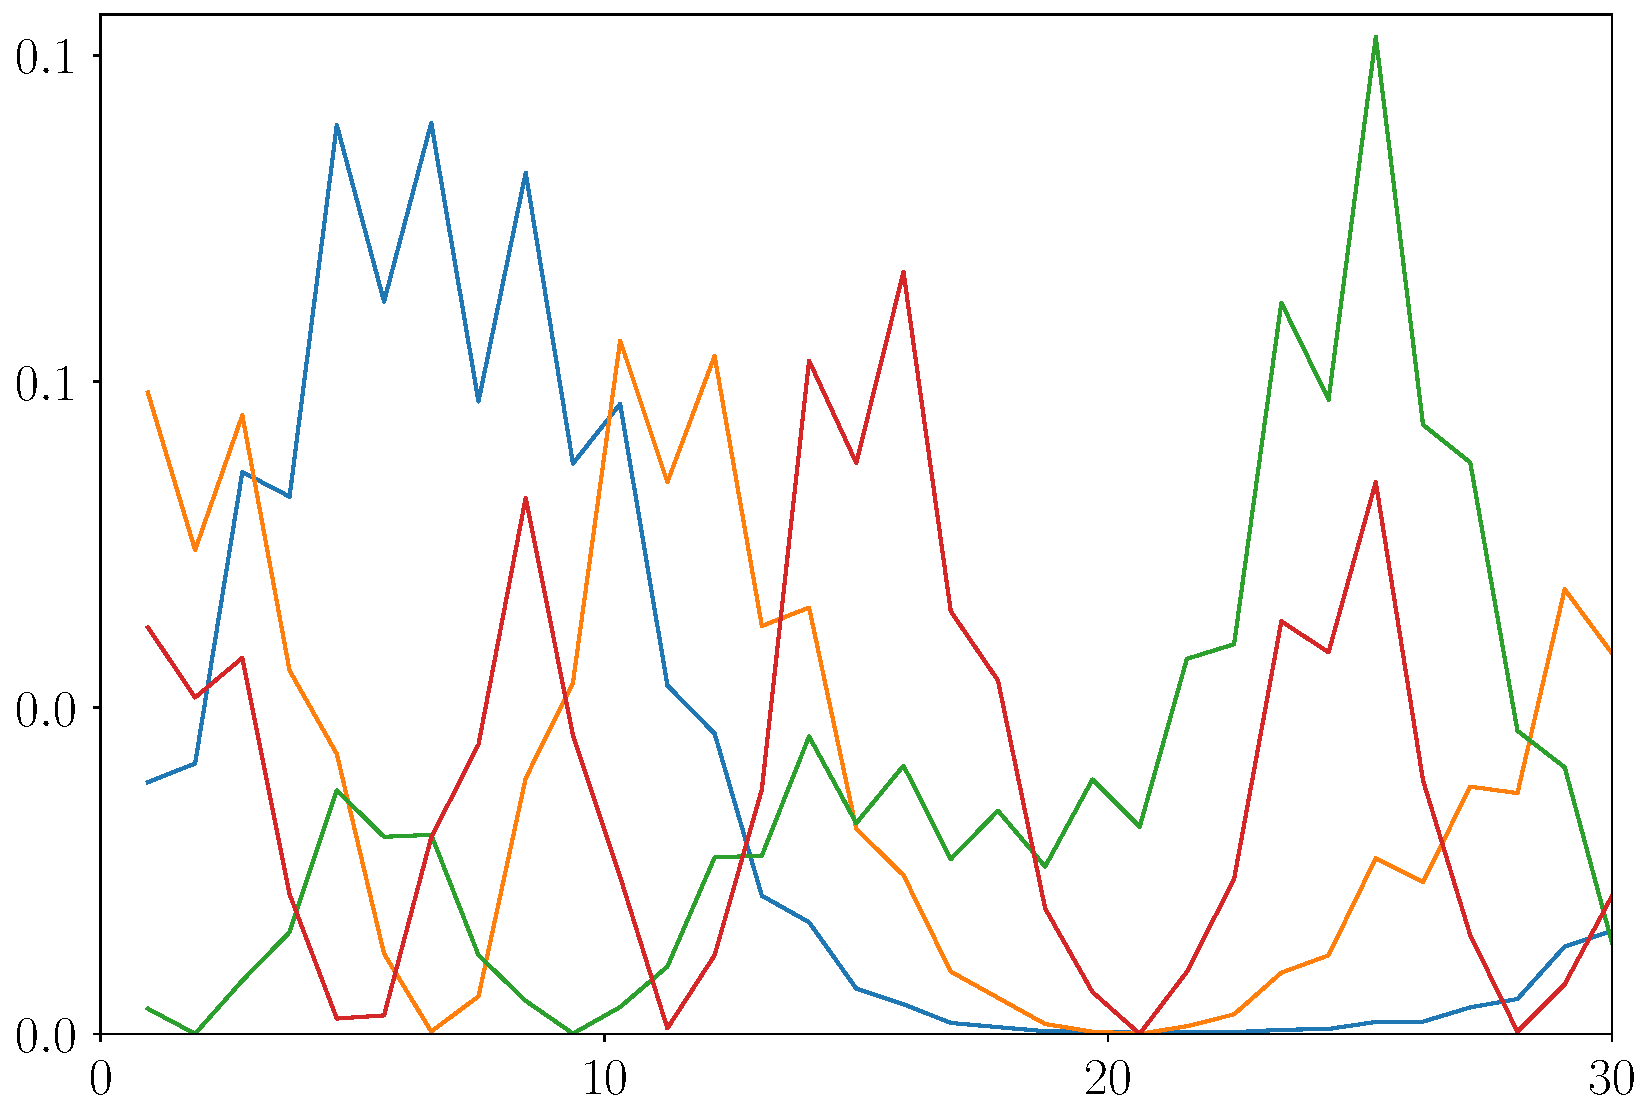
\includegraphics[width=\textwidth]{LHC_Eigenstates.pdf}
\end{figure}
\begin{figure}[H]
	\centering
	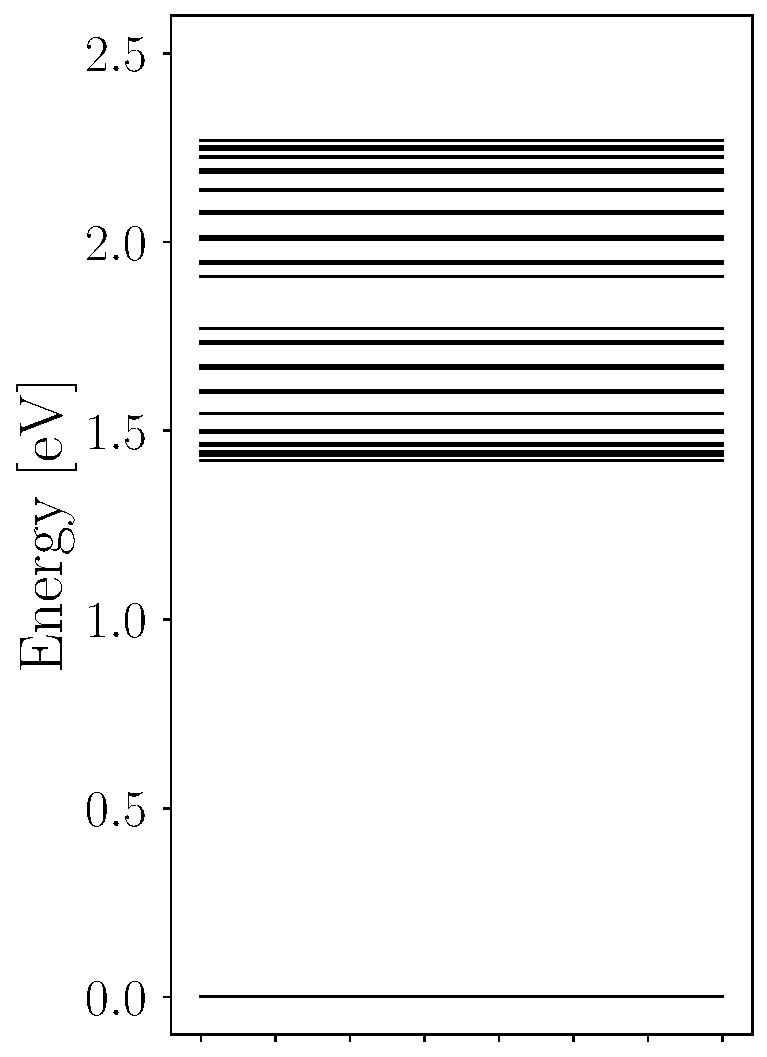
\includegraphics[width=6cm]{Purple_Bacteria_LHC_S0.pdf}
\end{figure}



\subsection{Exciton Energy Transfer}

\subsection{Supertransport}

\subsection{Electron Transfer}





\begin{figure}
	\centering
	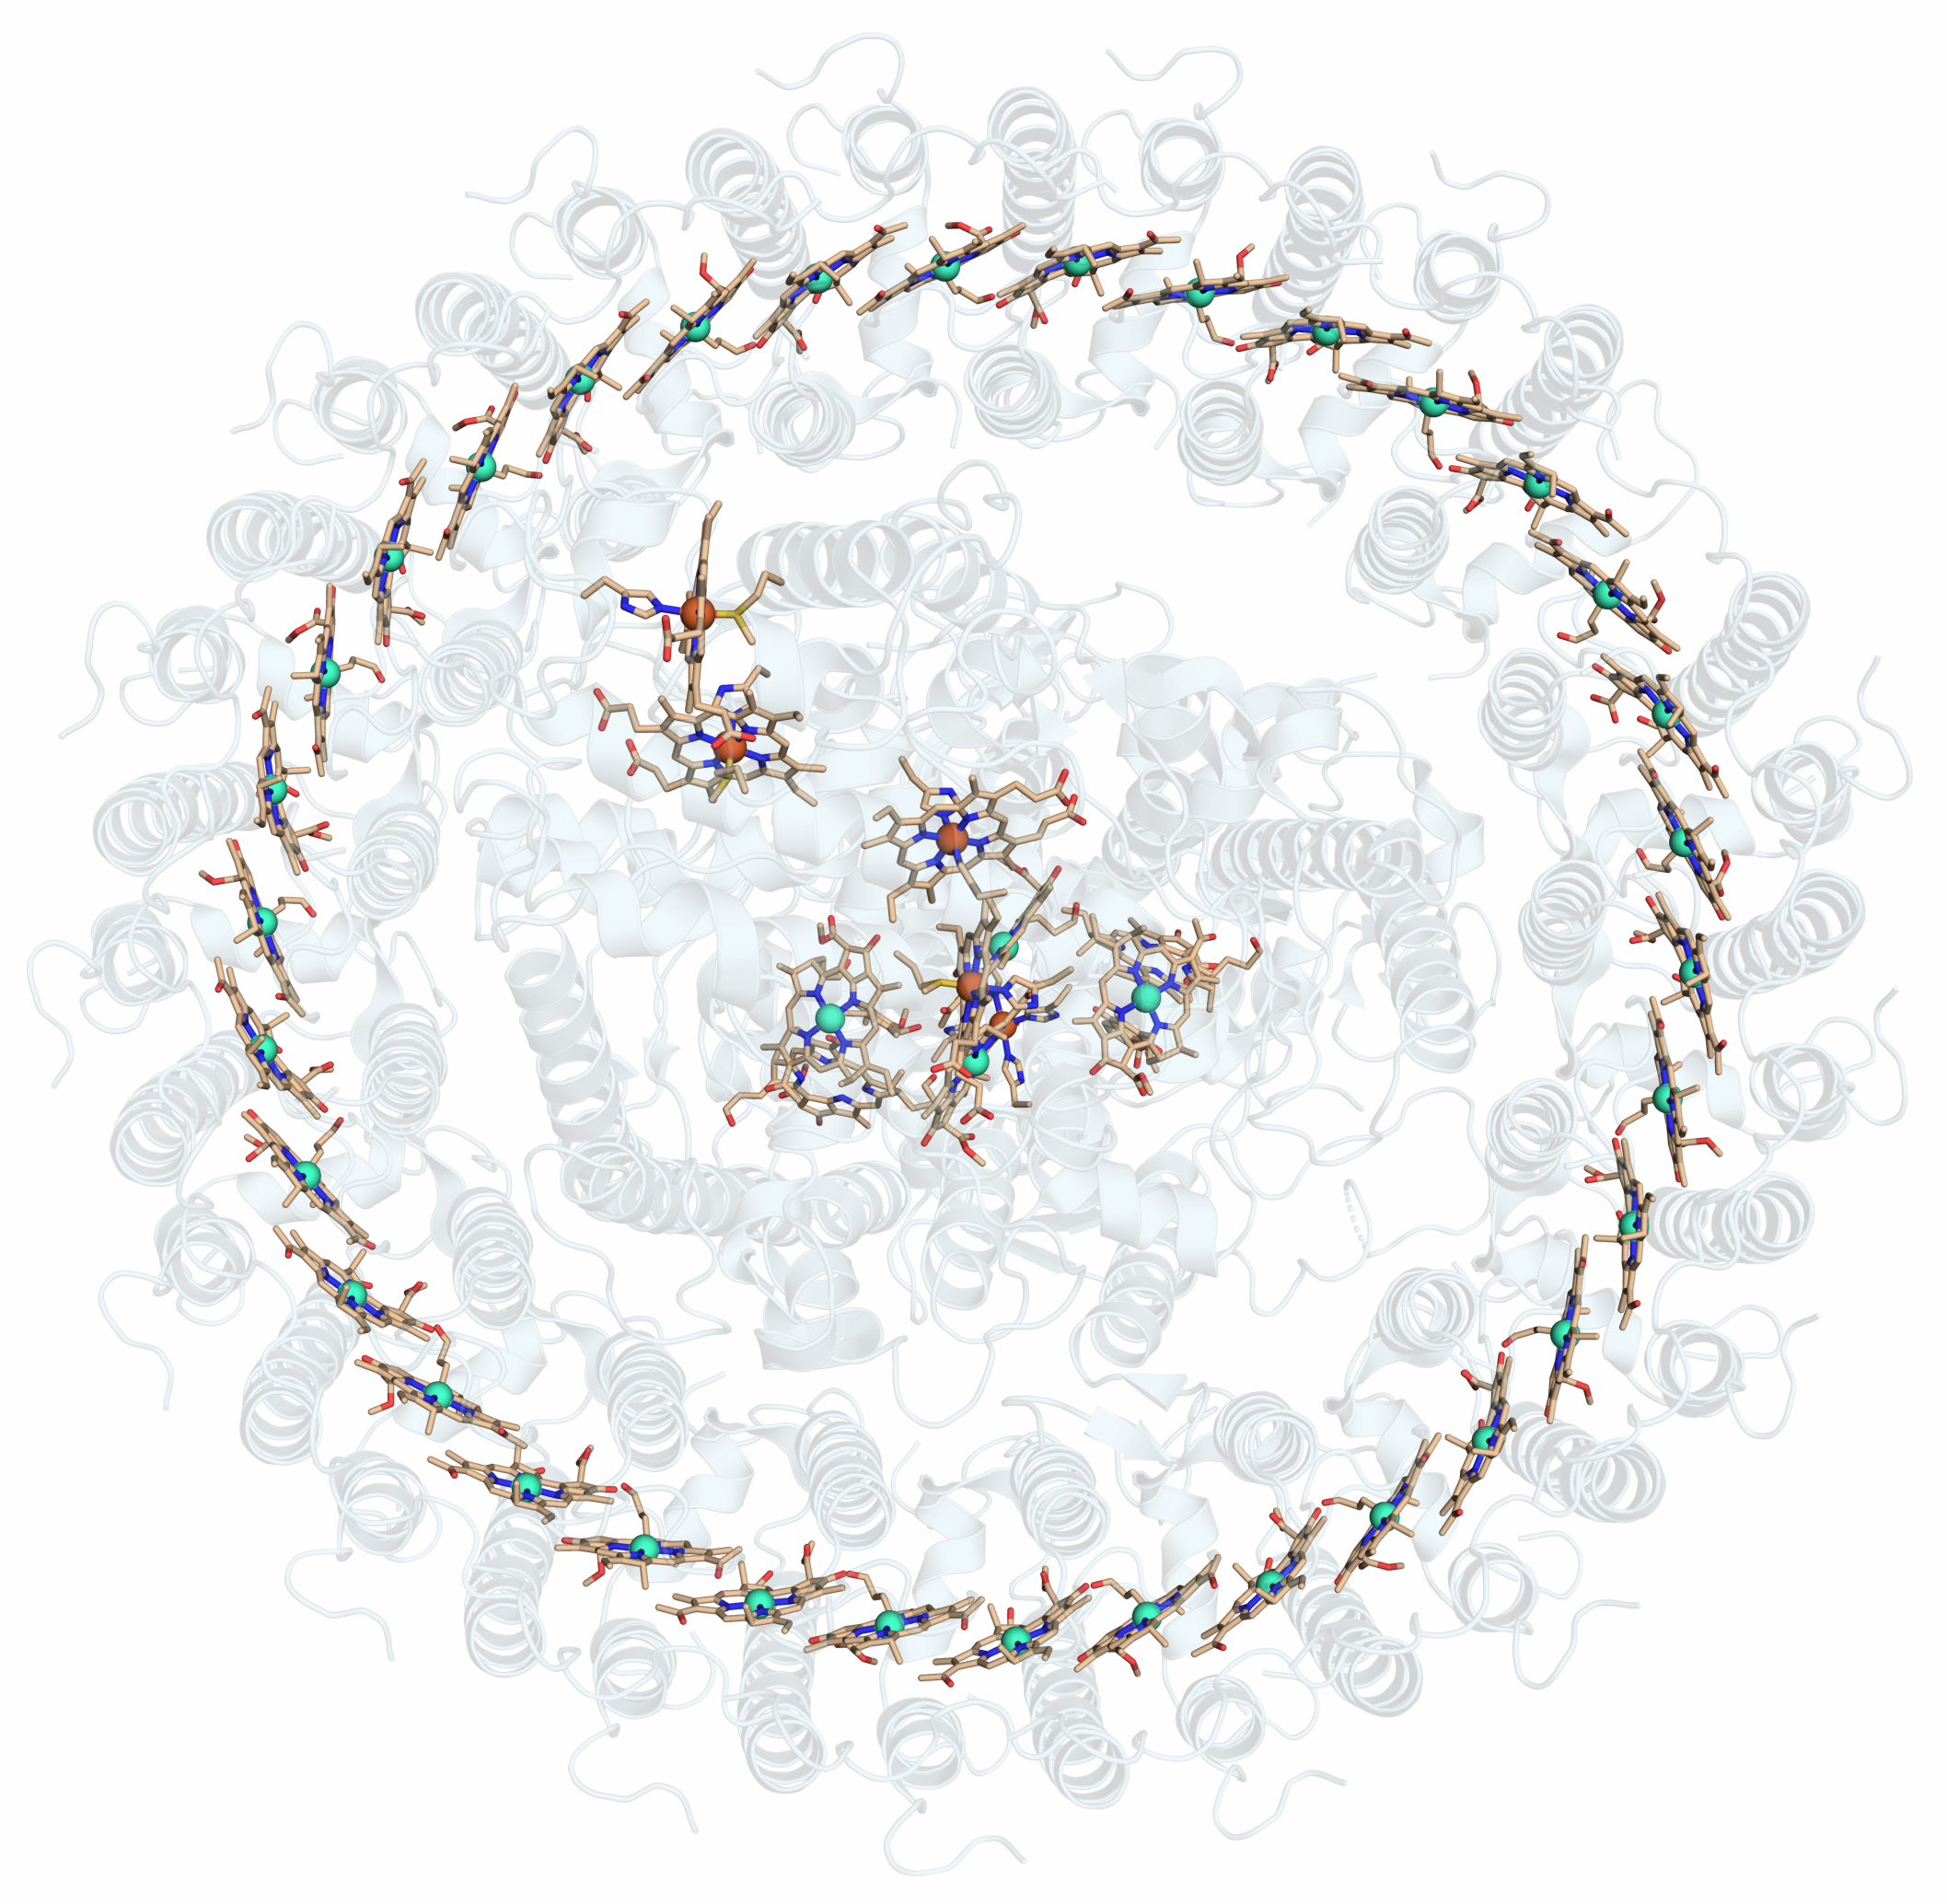
\includegraphics[width=\textwidth]{Purple_Bacteria_LHC_2.png}
\end{figure}

\begin{figure}
	\centering
	\includegraphics[width=\textwidth]{Purple_Bacteria_LHC_3.png}
\end{figure}













\chapter{Solid State Physics}

\section{Tight Binding Model}

\section{Kubo Formalism and Ohm's Law}

\url{https://physics.stackexchange.com/questions/332686/derivation-of-ohms-law-using-classical-and-quantum-model}\\
\url{https://iopscience.iop.org/article/10.1088/1742-6596/941/1/012047/pdf}\\
\url{https://de.wikipedia.org/wiki/Kuboformel}\\
























\chapter{Appendix}


\section{Hamiltonians in Second Quantization}
Electronic Structure Hamiltonian:
\begin{equation}
\hat{H} = \sum_{pq}h_{pq}\sum_{\sigma}\hat{a}^{\dagger}_{p\sigma}\hat{a}_{q\sigma}+\frac{1}{2}\sum_{pqrs}g_{pqrs}\sum_{\sigma\tau}\hat{a}_{p\sigma}^{\dagger}\hat{a}_{r\tau}^{\dagger}\hat{a}_{s\tau}\hat{a}_{q\sigma}
\end{equation}
Frenkel Exciton Hamiltonian:
\begin{equation}
\hat{H}=\sum_{m=1}^{N}\varepsilon_{m}\hat{a}^{\dagger}_{m}\hat{a}_{m}+\sum_{n<m}^{N}J_{mn}(\hat{a}^{\dagger}_{m}\hat{a}_{n}+\hat{a}_{n}^{\dagger}\hat{a}_{m})
\end{equation}
Hamiltonian of a two-level atom interacting with a $k$-mode electromagnetic field:
\begin{equation}
\hat{H}=\sum_{j}E_{j}\hat{a}_{j}^{\dagger}\hat{a}_{j} +\sum_{k}\hbar\omega_{k}\hat{a}_{k}^{\dagger}\hat{a}_{k} +\hbar\sum_{i,j,k}\hat{a}_{i}^{\dagger}\hat{a}_{j}\big(g_{ijk}\hat{a}_{k}+g_{ijk}^{*}\hat{a}_{k}^{\dagger}\big)
\end{equation}
Cooper Pair Hamiltonian:
\begin{equation}
\hat{H}=\sum_{k}\varepsilon_{k}\hat{a}_{k}^{\dagger}\hat{a} +\sum_{k}\Delta(\hat{a}^{\dagger}_{k}\hat{a}^{\dagger}_{-k}+\hat{a}_{k}\hat{a}_{-k})
\end{equation}
Hubbard model Hamiltonian:
\begin{equation}
\hat{H}= U\sum_{i}\hat{a}_{i\uparrow}^{\dagger}\hat{a}_{i\uparrow}\hat{a}^{\dagger}_{i\downarrow}\hat{a}_{i\downarrow}-t\sum_{\langle ij\rangle,\sigma}(\hat{a}_{i\sigma}^{\dagger}\hat{a}_{j\sigma}+\hat{a}_{j\sigma}^{\dagger}\hat{a}_{i\sigma})
\end{equation}



\url{https://en.wikiversity.org/wiki/Open_Quantum_Systems/The_Quantum_Optical_Master_Equation}\\
\url{https://arxiv.org/pdf/1708.06797.pdf}\\
\url{https://en.wikipedia.org/wiki/Lindbladian}\\
\url{https://en.wikipedia.org/wiki/Redfield_equation}\\
\url{https://physics.stackexchange.com/questions/229319/relationship-between-the-lindblad-equation-and-redfield-equation}\\
\url{https://qutip.org/docs/latest/guide/dynamics/dynamics-bloch-redfield.html}














\end{document}